\documentclass[twoside,english]{uiofysmaster/uiofysmaster}

\usepackage[toc,titletoc,title,page]{appendix} %to add appendices (and have them in toc)
\usepackage[utf8]{inputenc}
%\usepackage{mhchem} %latex chemistry symbols
\usepackage{blindtext} %to fill in dummy text
%\usepackage{cite} %to have multiple citations in one \cite{key1,key2,..} -do not use with natbib!!
\usepackage{tcolorbox} %to have boxes w color around text and math mode
\usepackage{enumitem} %to reduce vertical spacing in enumerate
\usepackage{tabu} % to set tables to page width
%\usepackage{aas_macros}

\usepackage[sort&compress,square,comma,numbers]{natbib} %to use \citet, now mixed with [nr]
\usepackage[nottoc]{tocbibind}

\usepackage{float} 
\usepackage[export]{adjustbox}
\usepackage{subcaption}
\newcommand{\blank}[1]{\hspace*{#1}} % move figures by \blank{}
\usepackage{pdfpages}
\usepackage{tikz}
\usetikzlibrary{
	arrows, 
	shapes.callouts,
	decorations.pathreplacing,
	decorations.pathmorphing,
	calc
}
\usepackage{stackengine}

%---

\interfootnotelinepenalty=10000 % to force footnotes to NOT run over to the next page

%---
% to reduce space around table of contents (to fit everything into one page): 
\usepackage{tocloft}
\setlength{\cftbeforetoctitleskip}{0pt}
\setlength{\cftaftertoctitleskip}{0pt}
%---

\usepackage{epigraph}
\setlength\epigraphwidth{11cm}
\setlength\epigraphrule{0pt}

%---
\newcommand{\Sm}{$^{140}$Sm} % making it faster to write Sm140
\newcommand{\Pb}{$^{208}$Pb} 
\newcommand{\bd}{$\beta$-decay} % making it faster to write 
\newcommand{\ga}{$\gamma$}
\newcommand{\MBOU}{MAR\belowbaseline[-2pt]{a}B\stackinset{l}{3pt}{b}{-3pt}{O}{O}\,U}
\newcommand{\Ba}{$^{133}$Ba}
\newcommand{\Eu}{$^{152}$Eu}

%---
% modifying color in code listings and some style
%\usepackage{color}

% The predefined color names are: 
% black, blue, brown, cyan, darkgray, gray, green, lightgray, lime, magenta, olive, orange, pink, purple, red, teal, violet, white, yellow.
 
%\definecolor{codegreen}{rgb}{0,0.6,0} % too flashy
\definecolor{codegreen}{rgb}{0.0, 0.42, 0.24} % less flashy so comments not take all attention
\definecolor{codegray}{rgb}{0.5,0.5,0.5}
\definecolor{codepurple}{rgb}{0.58,0,0.82}
%\definecolor{codepurple}{rgb}{1.0, 0.0, 0.22} %carminered, could try it 
%\definecolor{backcolour}{rgb}{0.95,0.95,0.92} % original suggestion
\definecolor{backcolour}{rgb}{0.94, 0.97, 1.0}% aliceblue, not so flashy and not as ugly
\definecolor{LightGray}{gray}{0.95}
 
\lstdefinestyle{mystyle}{
    backgroundcolor=\color{backcolour},   
    commentstyle=\color{codegreen},
    %commentstyle=\color{codegray},    
    keywordstyle=\color{magenta},
    numberstyle=\tiny\color{codegray},
    stringstyle=\color{codepurple},
    basicstyle=\footnotesize,
    breakatwhitespace=false,         
    breaklines=true,                 
    captionpos=b,                    
    keepspaces=true,                 
    %numbers=left,     %removing line numbers in the code snippets               
    %numbersep=5pt,                  
    showspaces=false,                
    showstringspaces=false,
    showtabs=false,                  
    tabsize=2,
    %float=tp,
    %floatplacement=tbp
}
 
\lstset{
	style=mystyle,
	literate={~} {$\sim$}{1}
}
\renewcommand{\lstlistingname}{Code}
%---

%---
% new tcolorbox environment
% #1: tcolorbox options
% #2: color
% #3: box title
\newtcolorbox{mybox}[3][]
{
  colframe = #2!25,
  colback  = #2!10,
  coltitle = #2!20!black,  
  title    = #3,
  #1,
}

%% We need to redefine \autoref. We should use 
%% abbreviations inside the sentence and full names 
%% at the beginning of sentences. Additionally,
%% need to handle the plural cases.

\newcommand*{\Appendixautorefname}{Appendix} % Add Appendix to \autoref 

% \Autoref is for the beginning of the sentence
%\let\orgautoref\autoref
%\providecommand{\Autoref}
%        {\def\equationautorefname{Equation}%
%         \def\figureautorefname{Figure}%
%         \def\subfigureautorefname{Figure}%
%         \def\sectionautorefname{Section}%
%         \def\subsectionautorefname{Section}%
%         \def\subsubsectionautorefname{Section}%
%         \def\Itemautorefname{Item}%
%         \def\tableautorefname{Table}%
%         \orgautoref}

% \Autorefs is plural for the beginning of the sentence
%\providecommand{\Autorefs}
%        {\def\equationautorefname{Equations}%
%         \def\figureautorefname{Figures}%
%         \def\subfigureautorefname{Figures}%
%         \def\sectionautorefname{Sections}%
%         \def\subsectionautorefname{Sections}%
%         \def\subsubsectionautorefname{Sections}%
%         \def\Itemautorefname{Items}%
%         \def\tableautorefname{Tables}%
%         \orgautoref}

% \autoref is used inside a sentence 
% (this is a renew of the standard)
%\renewcommand{\autoref}
%        {\def\equationautorefname{Eq.}%
%         \def\figureautorefname{Fig.}%
%         \def\subfigureautorefname{Fig.}%
%         \def\sectionautorefname{Sec.}%
%         \def\subsectionautorefname{Sec.}%
%         \def\subsubsectionautorefname{Sec.}%
%         \def\Itemautorefname{item}%
%         \def\tableautorefname{Tab.}%
%         \orgautoref}

% \autorefs is plural for inside a sentence
%\providecommand{\autorefs}
%        {\def\equationautorefname{Eqs.}%
%         \def\figureautorefname{Figs.}%
%         \def\subfigureautorefname{Figs.}%
%         \def\sectionautorefname{Secs.}%
%         \def\subsectionautorefname{Secs.}%
%         \def\subsubsectionautorefname{Secs.}%
%         \def\Itemautorefname{items}%
%         \def\tableautorefname{Tabs.}%
%         \orgautoref}

% Make equations text be Eq. (ref)
\makeatletter
\def\tagform@#1{\maketag@@@{\ignorespaces#1\unskip\@@italiccorr}}
\let\orgtheequation\theequation
\def\theequation{(\orgtheequation)}
\makeatother

%% End of redefinition

%---


%\bibliography{references}

\author{Trond Wiggo Johansen}
\title{Coulomb excitation of $\textnormal{\Sm}$}
\date{September 2019}
 
% ----------------------------------------------------------------------------------------------------------------------
% ----------------------------------------------------------------------------------------------------------------------
%Equations
%
%The command \eqref{} works exactly like \ref{}, but it adds parantheses to a plain number.
%
%Figures and tables
%
%\autoref{} is a usefull command when refering to to figures and tables. The command creates a reference with additional text corresponding to the target's type. For example, the command \autoref{fig:myfigure} would create a hyperlink to the \label{fig:myfigure} command, wherever it is. Assuming that this label is pointing to a figure, the hyperlink would contain the text "Figure 1.1", or similar.

%Two basic citation commands, \citet and \citep for textual and parenthetical citations, respectively. …
%\citet{jon90} --> Jones et al. (1990)
%\citep{jon90} --> (Jones et al., 1990)
%\citet*{jon90} --> Jones, Baker, and Williams (1990)
%\citep*{jon90} --> (Jones, Baker, and Williams, 1990)


\begin{document}

% set space around equations
\setlength{\belowdisplayskip}{12pt} \setlength{\belowdisplayshortskip}{12pt}
\setlength{\abovedisplayskip}{12pt} \setlength{\abovedisplayshortskip}{12pt}

\maketitle

%Centering the front page, see: https://github.com/ComputationalPhysics/uiofysmaster

%%% ABSTRACT
\begin{abstract}


\end{abstract}


\begin{dedication}
To my family, for all their support and encouragement!

\end{dedication}

\begin{acknowledgements}
Supervisors Professor Andreas Görgen and Dr. Katarzyna Hady{\'{n}}ska-Kl{\c{e}}k

Nuclear Physics Group

Computational Physics Group, Professor Morten Hjorth-Jensen

CERN-ISOLDE, Dr. Liam Gaffney

Ville Virtanen from University of Jyväskylä for tips on scripts. 

Lillefy, FFU, Fysikkforeningen

My family

Morten, Alex and Astrid.

Ina, for pushing me towards excellence, I love you.

\subsection*{Collaboration details}


ENSAR2: European Nuclear Science and Applications Research - 2 \url{http://www.ensarfp7.eu}, UiO, ISOLDE, other contributors to the experiment?



  \vspace{1.5cm}
  
  \noindent\textit{Trond Wiggo Johansen}\\
  
  \noindent September, 2019


\vspace{1cm}

\begin{figure}[h]
	\begin{minipage}[b]{0.25\linewidth}
	\centering
		
\includegraphics[width=\textwidth]{uiofysmaster/figures/apollonseglet/Apollonseglet/UiO_Segl_150dpi.png}
	\end{minipage}
	\hspace{4.8cm}
	\begin{minipage}[b]{0.45\linewidth}
	\centering
		
\includegraphics[width=\textwidth]{Images/ISOLDE-logo.png}
	\end{minipage}
\end{figure}


\end{acknowledgements}


\tableofcontents


% ----------------------------------------------------------------------------------------------------------------------
% ----------------------------------------------------------------------------------------------------------------------

\chapter{Introduction}
\textcolor{red}{+ Motivation}


The experiment has been done before, with lower energy (and another target), Malin Klintefjord. \url{http://urn.nb.no/URN:NBN:no-56121} \newline
 
Malin Klintefjord PhD thesis \cite{Klintefjord} with the three papers \cite{Klintefjord2015}, \cite{Samorajczyk2015} and \cite{Klintefjord2016} on \Sm.
 
\bigskip
 
Experiment conducted 8th - 14th of August 2017.

\bigskip

Expect to measure transition probabilities $B(E2)$ and quadrupole moment (nuclear deformation). 

\bigskip

\textcolor{Magenta}{Tilbakemelding: \newline 
old REX-ISOLDE post-accelerator limited to 2.8 MeV/u (low Coulomb excitation cross section, low probability for multi-step excitation). Mo target was chosen to maximize cross section at this energy, and to normalize B(E2; $0^+ \rightarrow 2^+$) value in \Sm\ to the well-known B(E2) value for the target. \newline
New HIE-ISOLDE: energies up to 10 MeV/u $\implies$ we can choose high-Z target (Pb) $\implies$ high Coulex cross section, especially for multi-step. Also: B(E2) for \Sm\ now known from previous experiment (and a lifetime measurement) $\implies$ no need for normalization: we can use the known B(E2; $0^+ \rightarrow 2^+$) to nomalize the transition probabilities for the higher-lying transitions. Chosen 4.7 MeV/u as the highest possible energy that is safe for Pb (distance of closest approach large enough to exclude nuclear interaction.)} \newline


All of my scripts are available in my GitHub repository found at \\ \url{https://github.com/wiggoen/MasterThesis}.

\bigskip

\textbf{COULEX links:}
\begin{itemize}
	\item \url{https://www.researchgate.net/profile/Jacek_Wojciechowski/publication/268366137_Application_of_Genetic_Algorithm_with_Real_Representation_to_COULEX_Data_Analysis/links/54b913850cf269d8cbf72ed4.pdf}
	\item \url{https://core.ac.uk/download/pdf/76649116.pdf}
	\item \url{http://oregonstate.edu/instruct/ch374/ch418518/Chapter%2010%20NUCLEAR%20REACTIONS.pdf}
\end{itemize}



% ----------------------------------------------------------------------------------------------------------------------
% ----------------------------------------------------------------------------------------------------------------------

\chapter{Theory}
table of nuclides (HFB-style): \url{http://www-phynu.cea.fr/science_en_ligne/carte_potentiels_microscopiques/carte_potentiel_nucleaire_eng.htm}

$\beta-\gamma$ triangle: \url{http://www-phynu.cea.fr/science_en_ligne/carte_potentiels_microscopiques/noyaux/zz62/zz62nn78all_eng.html}

\begin{table}[ht] 
    \centering 
    \caption{Values of the fundamental physical constants from the National Institute of Standards and Technology (NIST) Physics Laboratory \cite{units}.}
	% Data for the unit table
\begin{tabular}{llll}
\hline
Quantity                 & Symbol & Numerical value                    & Unit \\
\hline
Speed of light in vacuum & $c$    & $299792458$                        & m/s                                       \\
Elementary charge        & $e$    & $1.602176634 \cdot 10^{-19}$       & C = $\text{A}\cdot\text{s}$               \\
Electron volt            &  eV    & $1.602176634 \cdot 10^{-19}$       & J = $\text{kg}\cdot\text{m}^2/\text{s}^2$ \\
Atomic mass unit         & $u$    & $1.66053906660(50) \cdot 10^{-27}$ & kg                                        \\
\hline
\end{tabular}
	\label{tab:units}
\end{table}

\bigskip

Isotope notation:
\begin{align*}
	^A_Z\text{X}_N^Q
\end{align*}
where $X$ is the chemical symbol of the element, $A$ is the nucleon number (mass number, $A = Z + N$), $Z$ is the atomic number (proton number), $N$ is the neutron number and $Q$ is the charge ($Q = Z$ protons $- ~i$ electrons). 

\bigskip

Why CoulEx? \url{https://iks32.fys.kuleuven.be/wiki/brix/images/5/58/10_20151123_Illana_BriX15_web.pdf} \newline


Magic numbers: 2, 8, 20, 28, 50, 82, 126 \newline
Maria Goeppert Mayer “discovered” them in $\sim$1945. Observation of periodicity in binding energy $\implies$ shell model for nuclei. \newline
Eugene Wigner believed in liquid-drop model, did not trust new theory $\implies$ called these numbers “magic”. \newline
Source: \url{https://ocw.mit.edu/courses/nuclear-engineering/22-02-introduction-to-applied-nuclear-physics-spring-2012/lecture-notes/MIT22_02S12_lec01.pdf}

\bigskip

Quadrupole deformation of nuclei. \newline

Shape coexistence possible for certain regions of $N$ and $Z$.

\bigskip

- triaxial shape / shape coexistence \newline
- benchmark for theoretical models \newline
- transition probabilities and quadrupole moments between several excited states are not known \newline
- fundamental research

\bigskip

COULEX: \newline
- nucleus excited by electromagnetic interaction. \newline
- de-excitation $\rightarrow$ gamma

\bigskip

\textcolor{Magenta}{Tilbakemelding: \newline 
shape coexistence often found near closed shells. Example: neutron deficient Hg nuclei (Z = 80 just below 82 shell closure, N $\sim$ 104: neutron mid-shell). \newline
\Sm: N = 78, just below N = 82 shell closure, Z = 62: mid-shell. \newline
Typical indication for shape coexistence: $0^+$ states (often at low energy). \newline 
\Sm\ was thought to have a low-lying $0^+$ state [Firestone], but this state was shown to be $2^+$ [Suoranczyk?]. Indication for $0^+$ states around 1.5 MeV. \newline 
One of the objectives of this experiment: clarify the nature/structure of these $0^+$ states. \newline 
Shape transition: Sm-144 (Z = 62, N = 82) spherical. Adding neutrons: transition of N = 90 from spherical to prolate deformed $\rightarrow$ shape-phase transition, so called X(5) critical-point symmetry. \newline
Taking out neutrons: very neutron-deficient Sm nuclei are also prolate deformed (e.g. Sm-132), but for \Sm: indication for triaxiality/\ga-softness [Klintefjord] $\rightarrow$ another form of shape-phase transition/critical point behavior $\implies$ E(5) [Iachello?]. \Sm\ could be one of the best examples for E(5) symmetry $\implies$ need transition probabilities from higher-lying states to confirm.} \newline


\textcolor{red}{Some suggestions:} \newline
$\bullet$ general things about nuclei shapes \newline
- multipole expansion, shape parameters (5 parameters, 3 for space, 2 for deformation $\beta$, \ga), ... \newline
- quadrupole moments: intrinsic (body-fixed frame), spectroscopic (lab frame)  \newline
- transition probabilities, el.magn. matrix elements  \newline
- rotations and vibrations $\rightarrow$ energy spectra, B(E2) values  \newline
- Casten triangle (spherical vibrator, deformed rotor, \ga-soft + X(5), E(5)), expected spectrum for E(5) nuclei \newline

$\bullet$ the basics of Coulomb excitation (COULEX)


\bigskip

LISE++ \cite{LISE}

\begin{table}[ht] 
    \centering 
    \caption{LAB vs. CM. Based on LAB input angles from $\theta_b$ and $\theta_t$. From LISE++ kinematics calculator (reaction from the middle of the target).}
	\label{tab:LABvsCM}
    \begin{subtable}{0.45\textwidth}
    		\centering
		\caption{$\theta_b \in [22.0^\circ, 56.7^\circ]$.}
	 	\label{tab:LABvsCM_b}
	 	% Data for the LAB vs CM angle table
\begin{tabular}{ccc}
\hline
\multicolumn{2}{c}{LAB} & CM  \\
$\theta_b$ [$^\circ$]   &  $\theta_t$ [$^\circ$]  &  $\theta_b^{'}$ [$^\circ$]  \\
\hline
22.0                    &  71.7                   &  36.6                       \\
26.0                    &  68.4                   &  43.2                       \\
29.1                    &  65.9                   &  48.2                       \\
32.2                    &  63.4                   &  53.3                       \\
35.2                    &  60.9                   &  58.1                       \\
37.9                    &  58.8                   &  62.4                       \\
40.4                    &  56.8                   &  66.3                       \\
42.8                    &  54.9                   &  70.1                       \\
45.0                    &  53.2                   &  73.5                       \\
47.1                    &  51.6                   &  76.7                       \\
49.0                    &  50.2                   &  79.6                       \\
50.7                    &  48.9                   &  82.1                       \\
52.4                    &  47.6                   &  84.7                       \\
53.9                    &  46.5                   &  86.9                       \\
55.3                    &  45.5                   &  88.9                       \\
56.7                    &  44.5                   &  91.0                       \\
\hline
\end{tabular}
	\end{subtable}
	\begin{subtable}{0.45\textwidth}
		\centering
		\caption{$\theta_t \in [22.0^\circ, 56.7^\circ]$.}
		\label{tab:LABvsCM_t}
		% Data for the LAB vs CM angle table
\begin{tabular}{ccc}
\hline
\multicolumn{2}{c}{LAB} & CM  \\
$\theta_b$ [$^\circ$]   &  $\theta_t$ [$^\circ$]  &  $\theta_b^{'}$ [$^\circ$]  \\
\hline
{\color{red}40.6}  &  {\color{red}56.7}  &  {\color{red}66.6}   \\
{\color{red}42.3}  &  {\color{red}55.3}  &  {\color{red}69.4}   \\
{\color{red}44.2}  &  {\color{red}53.9}  &  {\color{red}72.2}   \\
{\color{red}46.1}  &  {\color{red}52.4}  &  {\color{red}75.2}   \\
{\color{red}48.3}  &  {\color{red}50.7}  &  {\color{red}78.6}   \\
{\color{red}50.6}  &  {\color{red}49.0}  &  {\color{red}82.0}   \\
{\color{red}53.1}  &  {\color{red}47.1}  &  {\color{red}85.8}   \\
{\color{red}56.0}  &  {\color{red}45.0}  &  {\color{red}90.0}   \\
			59.1   &  			  42.8   &  		    94.4    \\
		    62.5   &  			  40.4   &  		    99.2    \\
		    66.1   &  			  37.9   &  		    104.2   \\
		    70.2   &  			  35.2   &  		    109.6   \\
		    75.0   &  			  32.2   &  		    115.6   \\
		    80.2   &  			  29.1   &  		    121.8   \\
		    85.8   &  			  26.0   &  		    128.0   \\
		    93.8   &  			  22.0   &  		    136.0   \\
\hline
\end{tabular}

	\end{subtable}
\end{table}


\begin{figure}[ht]
	\centering
	\begin{subfigure}{\textwidth}
		%%
%% Laboratory frame
%%
\begin{tikzpicture}
    % Definitions
    \coordinate (Bleft)  at (-5,0.5);
    \coordinate (Bright) at (5,0.5);
    \coordinate (origo)  at (0,0);
    \coordinate (Tleft)  at (-5,-0.5);
    \coordinate (Tright) at (5,-0.5);
    \coordinate (Bup)    at (2,3);
    \coordinate (Tstart) at (0,-0.5);
    \coordinate (Tdown)  at (1.5,-1.5);
    % Lines
    \draw[dotted] (Tleft) -- (Tright);
    \draw[dotted] (Bleft) -- (Bright);
    \draw[dotted] (origo) -- (Bup);   % particle angle line
    \draw[dotted] (origo) -- (2,-2);  % target angle line
    % Particle paths
    \draw[red,loosely dashed]  (Bleft)  .. controls (-0.5,0.5) and (0.5,0.5) .. (Bup);
    \draw[blue,loosely dashed] (Tstart) .. controls (0.5,-0.5) and (1,-1)    .. (Tdown);
    % Impact parameter
    \draw[<->, >=stealth] (-3,0.5) -- node[left] {b} (-3,-0.5);
    % Center of mass
    \draw[fill=black] (origo) circle[radius=0.07cm] node {};
    \draw[->, >=stealth] (origo) -- (1.5,0) node[right] {$\textbf{V}_{cm}$}; % CM help line
    % Angles
    \draw[->, >=stealth] (1.33,0.5) arc (0:57:1cm)  node[right,pos=0.6,outer sep=1mm] {$\theta_b$};
    \draw[->, >=stealth] (1.5,-0.5) arc (0:-46:1cm) node[right,pos=0.6,outer sep=1mm] {$\theta_t$};
    % Vectors
    \draw[->, >=stealth] (-4.78,0.5) -- ++(1,0)        node[below,pos=0.7,outer sep=0.5mm] {$\textbf{u}$};
    \draw[->, >=stealth] (Bup)       -- ++(0.5,0.75)   node[right,pos=0.4,outer sep=0.6mm] {$\textbf{v}_b$};
    \draw[->, >=stealth] (Tdown)     -- ++(0.66,-0.66) node[right,pos=0.3,outer sep=1.2mm] {$\textbf{v}_t$};
    % Particles
    \draw[draw=blue,fill=blue!20] (Tdown)  circle[radius=0.25cm] node {t};
    \draw[draw=blue,fill=blue!20] (Tstart) circle[radius=0.25cm] node {t};
    \draw[draw=red,fill=red!20]   (Bleft)  circle[radius=0.22cm] node {b};
    \draw[draw=red,fill=red!20]   (Bup)    circle[radius=0.22cm] node {b};
    % Coordinate system 
    \coordinate (CSP) at (-4,1.5);
    \draw[->, >=stealth] (CSP) -- ++(1,0) node[below, pos=0.9] {x};
    \draw[->, >=stealth] (CSP) -- ++(0,1) node[left, pos=0.9]  {y};
    % Vertical alignment with CM frame
    \node[] at (-7.08,0) {};
    % Vertical space from caption text
    \node[] at (0,-2.5) {};
\end{tikzpicture}
		\caption{Scattering in the laboratory (LAB) frame. A small angle $\theta_b$ means forward scattering of the beam, a larger distance between the beam particle and the target particle, a weaker electromagnetic (EM) field and less excitation probability. A large angle $\theta_b$ means backward scattering of the beam, a closer distance between the beam particle and the target particle, a stronger EM field and a higher excitation probability.}
		\label{fig:LAB}
	\end{subfigure}
	\begin{subfigure}{\textwidth}
		%%
%% Center of mass frame
%%
\begin{center}
\begin{tikzpicture}
    % Definitions
    \coordinate (Bleft)  at (-5,0.5);
    \coordinate (Bright) at (5,0.5);
    \coordinate (origo)  at (0,0);
    \coordinate (Tleft)  at (-5,-0.5);
    \coordinate (Tright) at (5,-0.5);
    \coordinate (Bup)    at (2,3);
    \coordinate (Tdown)  at (-2,-3);
    % Lines
    \draw[dotted] (Tleft)  -- (3.75,-0.5);
    \draw[dotted] (Tdown)  -- (Bup);    % 180 degree line
    \draw[dotted] (-0.5,0) -- (1.5,0);  % angle help line
    % Particle paths
    \draw[red,loosely dashed]  (Bleft)  .. controls (-0.5,0.5) and (0.5,0.5)   .. (Bup);
    \draw[blue,loosely dashed] (Tright) .. controls (0.5,-0.5) and (-0.5,-0.5) .. (Tdown);
    % Impact parameter
    \draw[<->, >=stealth] (-3,0.5) -- node[left] {b} (-3,-0.5);
    % Center of mass
    \draw[fill=black] (origo) circle[radius=0.07cm] node {};
    % Angles
    \draw[->, >=stealth] (1,0) arc (0:57:1cm) node[right, pos=0.6, outer sep=1mm] {$\theta_b^{'}$};
    % Vectors
    \draw[->, >=stealth] (-4.78,0.5) -- ++(1,0)        node[below, pos=0.7] {$\textbf{u}^{'}$};
    \draw[->, >=stealth] (4.75,-0.5) -- ++(-1,0)       node[below, pos=0.6] {-$\textbf{u}^{'}$};
    \draw[->, >=stealth] (Bup)       -- ++(0.5,0.75)   node[right, pos=0.4,outer sep=0.5mm] {$\textbf{v}_b^{'}$};
    \draw[->, >=stealth] (Tdown)     -- ++(-0.5,-0.75) node[right, pos=0.8,outer sep=0.5mm] {$\textbf{v}_t^{'}$};
    % Particles
    \draw[draw=blue,fill=blue!20] (Tdown)  circle[radius=0.25cm] node {t};
    \draw[draw=blue,fill=blue!20] (Tright) circle[radius=0.25cm] node {t};
    \draw[draw=red,fill=red!20]   (Bleft)  circle[radius=0.22cm] node {b};
    \draw[draw=red,fill=red!20]   (Bup)    circle[radius=0.22cm] node {b};
    % Coordinate system 
    \coordinate (CSP) at (-4,1.5);
    \draw[->, >=stealth] (CSP) -- ++(1,0) node[below, pos=0.9] {x'};
    \draw[->, >=stealth] (CSP) -- ++(0,1) node[left, pos=0.9] {y'};
    % Vertical space from LAB frame
    \node[] at (0,4.5) {};
\end{tikzpicture}
\end{center}
		\caption{Center of mass (CM) frame.}
		\label{fig:CM}
	\end{subfigure}
	\caption{LAB vs. CM frame.}
	\label{fig:LAB-CM}
\end{figure}

% ----------------------------------------------------------------------------------------------------------------------
% ----------------------------------------------------------------------------------------------------------------------
\newpage

\chapter*{\textcolor{red}{NOTES TO BE REMOVED!!}}
\section{Oppgaveteksten (skal fjernes!)}
\textcolor{red}{---------} \newline
\textcolor{red}{Oppgavens mål:} \newline
The ISOLDE facility at CERN has been upgraded to provide higher energies and intensities for radioactive ion beams. A new experiment to study 140Sm was performed in the summer of 2017. The goal of the experiment was to measure electromagnetic transition probabilities and electric quadrupole moments for several excited states in 140Sm by measuring Coulomb excitation probabilities. A large data set was obtained using silicon detectors to determine the energies and angles of scattered particles, and germanium detectors to measure gamma rays from excited states in 140Sm. \newline

The goal of the master thesis is to analyze the data from this experiment. The required tasks include development and improvement of data analysis software to determine Coulomb excitation yields. These yields will then, in a second step, be compared to theoretical calculations and transition probabilities and quadrupole moments will be extracted using chi-square minimization procedures. \newline


\textcolor{red}{Prosjektbeskrivelse (omfang 60 studiepoeng):} \newline
The shape of an atomic nucleus is determined by a delicate interplay between macroscopic (liquid drop) properties and microscopic shell effects. Nuclei with filled proton or neutron shells (i.e. magic nuclei) are generally spherical in shape, whereas nuclei with open shells gain energy by assuming a deformed shape. Depending on the occupation of specific orbitals, the nuclear shape can change drastically by adding or removing protons or neutrons. Certain nuclei exhibit shape coexistence, i.e. the coexistence of quantum states that correspond to different shapes. Because the shape of a nucleus is so sensitive to the underlying nuclear structure and to changes of the proton and neutron numbers, the excitation energy, or the angular momentum, observables related to the nuclear shape are used as benchmarks for theoretical models. 

Nuclei in the rare earth region, and in particular the chain of samarium isotopes, exhibit a variety of shape effects. The Sm isotope with closed neutron shell at N=82, 144Sm, is spherical in shape. Adding neutrons to 144Sm changes the deformation to an elongated (prolate) quadrupole shape. The transition from spherical to prolate shape, which occurs for 152Sm at N=90, can be interpreted as a shape-phase transition. Flattened (oblate) quadrupole shapes are predicted by theory to occur below the N=82 shell closure. An earlier experiment studying 140Sm at CERN-ISOLDE found triaxial shape for this isotope, i.e. a shape where all three principal axes of the ellipsoid have different lengths. 140Sm can therefore be considered to lie at the critical point of a phase transition from spherical to deformed, and from prolate to oblate shape. \newline

\textcolor{red}{Foreløpig tittel:} \newline
Coulomb excitation of 140Sm \newline


\textcolor{red}{Metoder som tenkes benyttet:} \newline
Multi-step Coulomb excitation with radioactive beam, isotope separation on-line technique, nuclear spectroscopy, particle-gamma and particle gamma-gamma coincidence analysis, advanced chi-square minimization procedures. \newline
\textcolor{red}{---------} \newline


\section*{\textcolor{red}{Sjekk sensorveiledning!!}}


\section*{\textcolor{red}{Fjern blå linker in-text før innlevering!!}}

\section*{\textcolor{red}{Experimental setup - other info sources}}
\begin{itemize}
	\item ISOL \& Post acceleration: \url{https://www.euroschoolonexoticbeams.be/site/files/nlp/LNP700_contrib2.pdf}
	\item ISOL RIB (2004): \url{http://accelconf.web.cern.ch/AccelConf/e04/PAPERS/TUXCH01.PDF}
	\item RIB (2017): \url{http://iopscience.iop.org/article/10.1088/1361-6471/aa990f/pdf}
	\item RIB: \url{http://publications.lib.chalmers.se/records/fulltext/175494/local_175494.pdf}
	\item RIB: \url{https://www.sciencedirect.com/science/article/pii/S0168583X02018864}
	\item Post-accelerated beams ISOLDE: \url{http://iopscience.iop.org/article/10.1088/1361-6471/aa78ca}
	\item PSB: \url{https://www.sciencedirect.com/science/article/pii/0168583X92959079}
	\item PSB: \url{https://home.cern/science/accelerators/proton-synchrotron-booster}
	\item RILIS ISOLDE: \url{https://www.sciencedirect.com/science/article/pii/S0168583X13008914}
	\item HIE-ISOLDE publications: \url{http://hie-isolde-project.web.cern.ch/hie-isolde-publications}
	\item Miniball pictures: \url{https://cds.cern.ch/record/844871?ln=en}
	\item The MINIBALL array \cite{MBarray}
\end{itemize}

\textcolor{red}{DAQ:}
\begin{itemize}
	\item \MBOU\ web page: \url{https://www-old.mll-muenchen.de/marabou/htmldoc/}
	\item \MBOU\ file formatting: \url{https://www-old.mll-muenchen.de/marabou/htmldoc/marabou/IOSpec.html}
\end{itemize}

\newpage

% ----------------------------------------------------------------------------------------------------------------------
% ----------------------------------------------------------------------------------------------------------------------

\chapter{Coulomb excitation experiment}
\section{ISOLDE at CERN}
The acronym ISOLDE stands for Isotope Separator On Line DEvice. ISOLDE is a Radioactive Ion Beam (RIB) facility at CERN in Meyrin, Switzerland.  \autoref{fig:accelerators} shows the CERN accelerator complex, where ISOLDE is located beside the Proton Synchrotron Booster (PSB). The facility can produce over 1000 different radionuclides to be used in a wide variety of experiments in nuclear physics, atomic physics, solid state physics, life sciences and fundamental interactions. Experiments have been performed at ISOLDE since 1967 and since 2001 experiments with post-accelerated RIBs have been conducted. The High Intensity and Energy upgrade (HIE-ISOLDE) have made it possible to deliver energies up to 10 MeV/$u$ in 2018 \cite{HIE-ISOLDE, ISOLDE-web, ISOLDE-facility}. 

Most of the around 4000 characterized nuclides are radioactive  \cite{CoN}. In many cases it is not possible to make radioactive nuclei targets and perform an experiment because of the short half-life of the nucleus of interest. To study these radioactive nuclei, RIBs are used on stable targets. One way of obtaining a RIB is to use the Isotope Separator On Line (ISOL) method. In the ISOL method, two accelerator systems is needed. The first accelerator is used to produce the radioactive atoms at rest, and the second accelerator is used to accelerate these atoms \cite{ISOL}. 

In RIB facilities the energy and intensity is generally lower compared to stable beam facilities. This makes it suitable for Coulomb excitation and particle transfer reactions. The beam is the isotope of interest and since it is traveling with a significant velocity ($v/c$ values of a few percent), the emitted \ga-rays from de-excitation may have large Doppler shifts. Since the detectors have a finite solid angle, it can lead to a sizable Doppler broadening. When the detection system has high granularity, the Doppler shifts and broadening can be corrected for. If the angle between the recoiling nucleus and the \ga-ray can be determined accurately, Doppler correction can be applied \cite{MB-spect}.

\begin{figure}[ht]
	\centering
	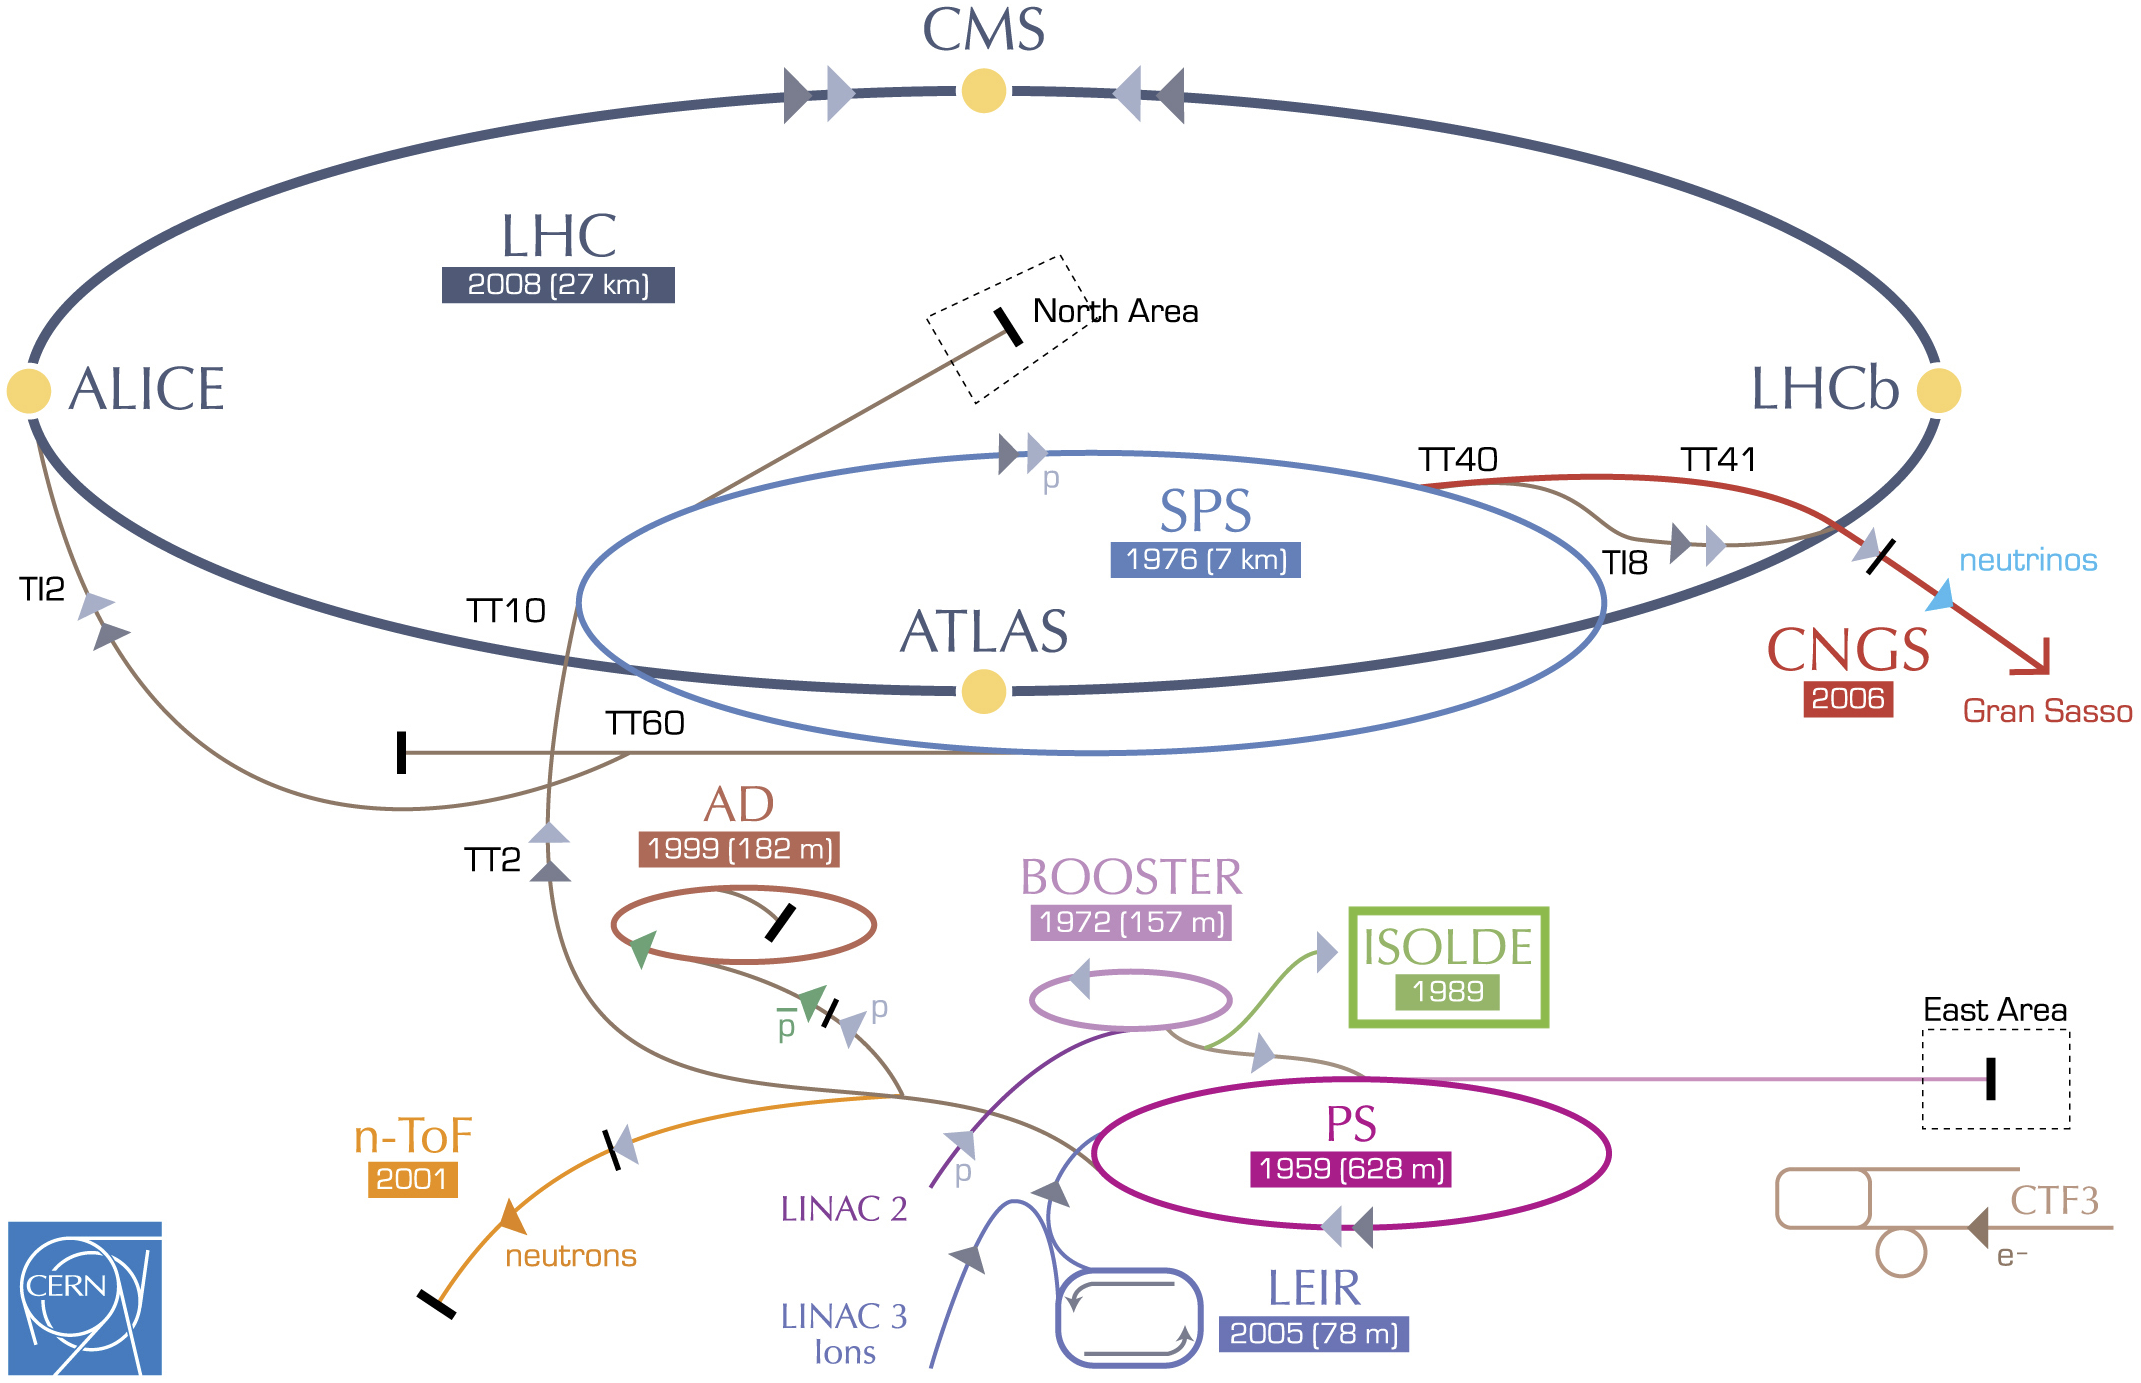
\includegraphics[width=\textwidth]{Images/CERN-accelerators.png}
	\caption{The CERN accelerator complex, adapted from \cite{CERN-AC}. ISOLDE, marked in the green box, gets accelerated protons from LINAC 2 and the PS Booster.}
	\label{fig:accelerators}
\end{figure}


\section{Experimental setup}
\subsection{Beam production}
\autoref{fig:Coulex} shows a sketch of the experimental setup used in the \Sm\ Coulomb excitation experiment. A continuous flow of accelerated proton beam bunches from the PSB comes into the ISOLDE facility and collide with a thick production target. The proton beam has an energy of 1.4 GeV and an intensity up to 2 $\mu$A. Two proton beam bunches is separated by 1.2 s \cite{TIF, TIF2013}. ISOLDE typically takes 50\% \cite{MB-spect} of all proton bunches form the PSB, the rest goes to the Large Hadron Collider (LHC) and other experiments shown in \autoref{fig:accelerators}. In the reaction between the proton beam and the production target, radioactive nuclides are produced in spallation, fission or fragmentation reactions (basically smashing the target into pieces) \cite{ISOLDE-web}. The production target is chosen from a stable region heavier than the nucleus of interest. In our experiment, a production target of tantalum (Ta, $Z = 73$) was used, producing the elements in the chart of nuclides up to Ta. A large amount of different isotopes is produced in this way, and the challenge is to extract the nucleus of interest. To obtain the nucleus of interest, we first have to use a method of selecting the atom of interest, and then the nucleus of interest. 

To get the atomic element of interest, one idea is to use a method of selective ionization and then a high voltage electrostatic field to extract the ions. Electronic transitions are characteristic for each chemical element. A laser with precisely tuned wavelength can obtain the photon energy that matches the electronic transition energies in the atom \cite{RILIS-web, RILIS2013}. Thus we can use one laser to excite an electron to a specific excited electron-state in the atom, a second laser to excite electrons further to another excited electron-sate and a third laser to kick out the electron. In this way we only ionize the atomic element of interest. There could be contaminants from surface ionization (atoms that collide with the walls of the ion source), but this is detectable. Using periods of laser on and off, we can detect the resulting contaminants in the beam. The Resonance Ionization Laser Ion Source (RILIS) is based on the method of step-wise (2-3 step) excitation and ionization of the atom. It is an element-selective process which is used to produce ion beams of the correct element \cite{RILIS}. In this experiment RILIS was used to select samarium (Sm) with atomic number $Z = 62$. 

At this point we have a continuous beam of Sm ions of 60 keV energy (the target is on a 60 kV high voltage platform) \cite{ISOLDE-web, TIF}. The next step in the process is to have mass separation, and we need to give the continuous beam a fine structure, because the post-accelerator cannot accept a continuous beam coming in, it accelerates bunches. The beam can collide in one of two target stations, either the General Purpose Separator (GPS) or the High Resolution Separator (HRS). The GPS has one bending magnet and can deliver beams of different masses ($\pm 13 \%$ of the central beam line mass) simultaneously into three beam lines, while the HRS has two bending magnets with high mass resolving power which delivers the beam into the main (central) beam line \cite{GPS, TIF}. In this experiment the GPS was used to select the isotope of Sm with mass number $A = 140$. 

Now we have a continuous beam of \Sm. The mass separator also gets rid of contaminants that come out of RILIS but have different mass. There could still be isobaric contaminants from surface ionization but luckily there is very little surface ionization for the neighboring elements of Sm. In the Radioactive beam EXperiment TRAP (REXTRAP) we collect the \Sm\ ions, so that we can release them in bunches that are matched to the fine structure of the LINear ACcelerator (LINAC). REXTRAP is a penning trap which has the tasks of accumulation, bunching and cooling of the RIB \cite{HIE-ISOLDE, REXTRAP1, REXTRAP2}. The ions are released in bunches and transfered to the REX Electron Beam Ion Source (REXEBIS).

REXEBIS is a charge breeder where the RIB is bred to a high charge state \cite{REXEBIS}, with a mass-to-charge ($A/q$) ratio typically between 2.5 and 4.5 \cite{Post-acc}. REXEBIS releases the beam with a certain energy through a mass separator and into the HIE-ISOLDE LINAC \cite{HIE-ISOLDE}. To accelerate the charged ions (the beam) to high energy, we need highly charged ions. The EBIS blasts off more electrons from Sm, which leaves the nucleus in a high charge state, going from \Sm$^{+1}$ to \Sm$^{+34}$ ($A/q \approx 4.1$). The longer the ions stay in REXEBIS, the higher the charge state becomes. We get a distribution of charge states, and we loose those that have the wrong charge state because the LINAC can only accept one charge state \cite{REX-web, HIE-web, EBIS2002, EBIS2010}.

The HIE-ISOLDE LINAC accelerates the beam of \Sm\ ($T_{1/2} = 14.82$ min) \textcolor{red}{with excellent purity} to 4.65 MeV/u (total energy 651 MeV) through the beam line, and magnets bend the beam into the Miniball spectrometer, where the particles and \ga-rays are detected. This experiment was one of the first Miniball experiments with the new upgraded superconducting accelerator. 

To have a successful experiment, the purity of the beam is of great importance. Contaminants in the beam can come from different sources  \cite{MB-spect}. From the primary target we can have:
\begin{itemize}
	\item isobaric contaminants which are inseparable by the mass separator because of the same mass number
	\item isotopes with an integer multiple of both mass and charge
\end{itemize}
and from stable isotopes the contaminants can come from:
\begin{itemize}
	\item buffer gas in REXTRAP (e.g. Ne, Ar)
	\item residual gas in REXEBIS (e.g. C, O)
	\item components of REXEBIS (e.g. La from the cathode)
\end{itemize}


\begin{figure}[ht]
	\centering
	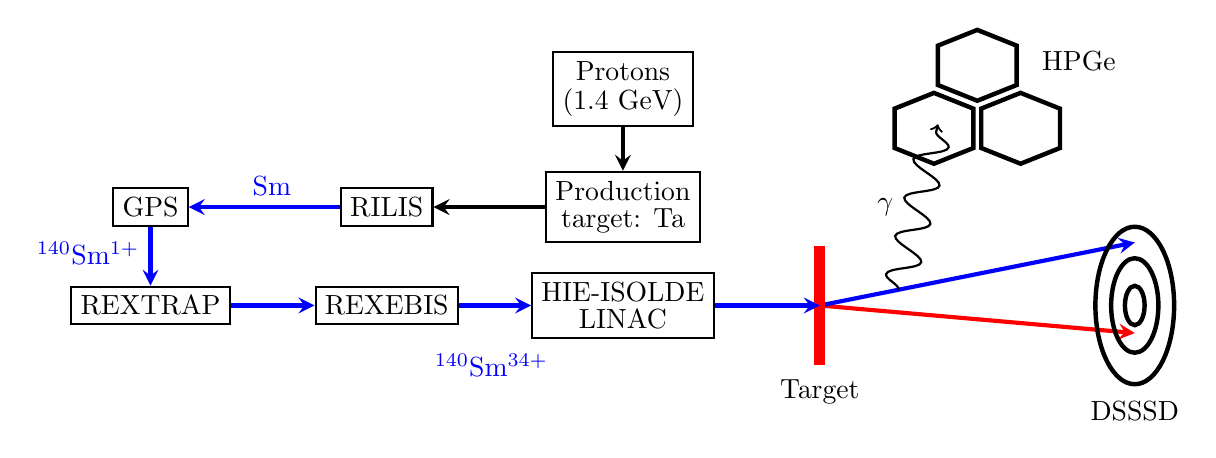
\begin{tikzpicture}
    % Definitions
    \coordinate (origo)   at (0,0);
    \coordinate (Protons) at (-2.5,2.75);
    \coordinate (GPS)     at (-8.5,1.25);
    \coordinate (RILIS)   at (-5.5,1.25);
    \coordinate (PTarget) at (-2.5,1.25);
    \coordinate (REXTRAP) at (-8.5,0);
    \coordinate (REXEBIS) at (-5.5,0);
    \coordinate (HILinac) at (-2.5,0);
    % Target and lines from target
    \draw[->,red,>=stealth,line width=1.5pt] (origo) -- (4,-0.35);
    \draw[->,blue,>=stealth,line width=1.5pt] (origo) -- (4,0.8);
    \draw[red, line width=4pt] (0,0.75) -- (0,-0.75) node[black, below] {Target};
    % Nodes
    \node(P)   at (Protons) [draw,thick] {\shortstack{Protons \\ (1.4 GeV)}};
    \node(G)   at (GPS)     [draw,thick] {GPS};
    \node(R)   at (RILIS)   [draw,thick] {RILIS};
    \node(PT)  at (PTarget) [draw,thick] {\shortstack{Production \\ target: Ta}};
    \node(RXT) at (REXTRAP) [draw,thick] {REXTRAP};
    \node(RXE) at (REXEBIS) [draw,thick] {REXEBIS};
    \node(LIN) at (HILinac) [draw,thick] {\shortstack{HIE-ISOLDE \\ LINAC}};
    % Arrows
    \draw[->,>=stealth,line width=1.5pt]      (P) -- (PT);
    \draw[->,>=stealth,line width=1.5pt]      (PT) -- (R);
    \draw[->,blue,>=stealth,line width=1.5pt] (R) -- (G) node[anchor=south, pos=0.45] {Sm};
    \draw[->,blue,>=stealth,line width=1.5pt] (G) -- (RXT) node[anchor=east, pos=0.45] {$^{140}$Sm$^{1+}$};
    \draw[->,blue,>=stealth,line width=1.5pt] (RXT) -- (RXE);
    \draw[->,blue,>=stealth,line width=1.5pt] (RXE) -- (LIN) node[anchor=north, pos=0.45, outer sep=5mm] {$^{140}$Sm$^{34+}$};
    \draw[->,blue,>=stealth,line width=1.5pt] (LIN) -- (origo);
    % CD 
    \draw[ultra thick] (4,0) ellipse [x radius=0.25cm,y radius=0.125cm, rotate=90];
    \draw[ultra thick] (4,0) ellipse [x radius=0.6cm,y radius=0.3cm, rotate=90];
    \draw[ultra thick] (4,0) ellipse [x radius=1cm,y radius=0.5cm, rotate=90] node[anchor=north, outer sep=11mm] {DSSSD};
    % HPGe
    %\draw (2,2.5) circle (1cm);
    \draw[ultra thick]  (0.95,2) -- ++(0.5,-0.2) -- ++(0.5,0.2) -- ++(0,0.5) -- ++(-0.5,0.2) -- ++(-0.5,-0.2) -- cycle;
    \draw[ultra thick] (1.5,2.8) -- ++(0.5,-0.2) -- ++(0.5,0.2) -- ++(0,0.5) -- ++(-0.5,0.2) -- ++(-0.5,-0.2) -- cycle;
    \draw[ultra thick]  (2.05,2) -- ++(0.5,-0.2) -- ++(0.5,0.2) -- ++(0,0.5) -- ++(-0.5,0.2) -- ++(-0.5,-0.2) -- cycle;
    \node[anchor=west] at (2.7,3.1) {HPGe};
    % Gamma
    \draw[->, decoration={snake,segment length=5mm,amplitude=2mm},decorate,thick] (1,0.2) -- (1.5,2.3) node[left, pos=0.5, outer sep=2mm] {$\gamma$};
\end{tikzpicture}
	\caption{The Coulomb excitation setup at ISOLDE (experiment code: IS558, which was titled Shape Transition and Coexistence in Neutron-Deficient Rare Earth Isotopes). Adapted from \cite{Klintefjord}.}
	\label{fig:Coulex}
\end{figure}


\subsection{Target}
As a target, \Pb\ with a thickness of 1.4 mg/cm$^2$ was chosen. The reason for the choice is that it is very hard to excite \Pb\ since it's doubly magic. We wanted the highest possible $Z ~(= 82)$ of a stable isotope to get maximum excitation probability. 

Since we don't need normalization (because we have the $B(E2, 0_1^+ \rightarrow 2_1^+$) from the previous experiment \cite{Klintefjord2016} and from lifetime measurement \cite{BelloGarrote2015}), we have chosen a target that is very hard to excite, so transitions from the target will not complicate the spectrum.

\Pb\ has no quadrupole deformation, the first excited state (2615 keV, $T_{1/2} = 16.7$ ps) is of octupole vibration ($J^\pi = 3^-$). If we are \textcolor{red}{lucky/unlucky?} we might see a little bit of this first excited state in the spectrum. This happens if the "collision" is almost head on, and the target hits one of the inner rings.

Unfortunately there was a finger print on the target, so even before beginning the experiment, we have some contamination (probably carbon).


\subsection{Miniball spectrometer}
\autoref{fig:MBSpect} shows an overview picture of the Miniball spectrometer. 

\begin{figure}[ht]
	\centering
	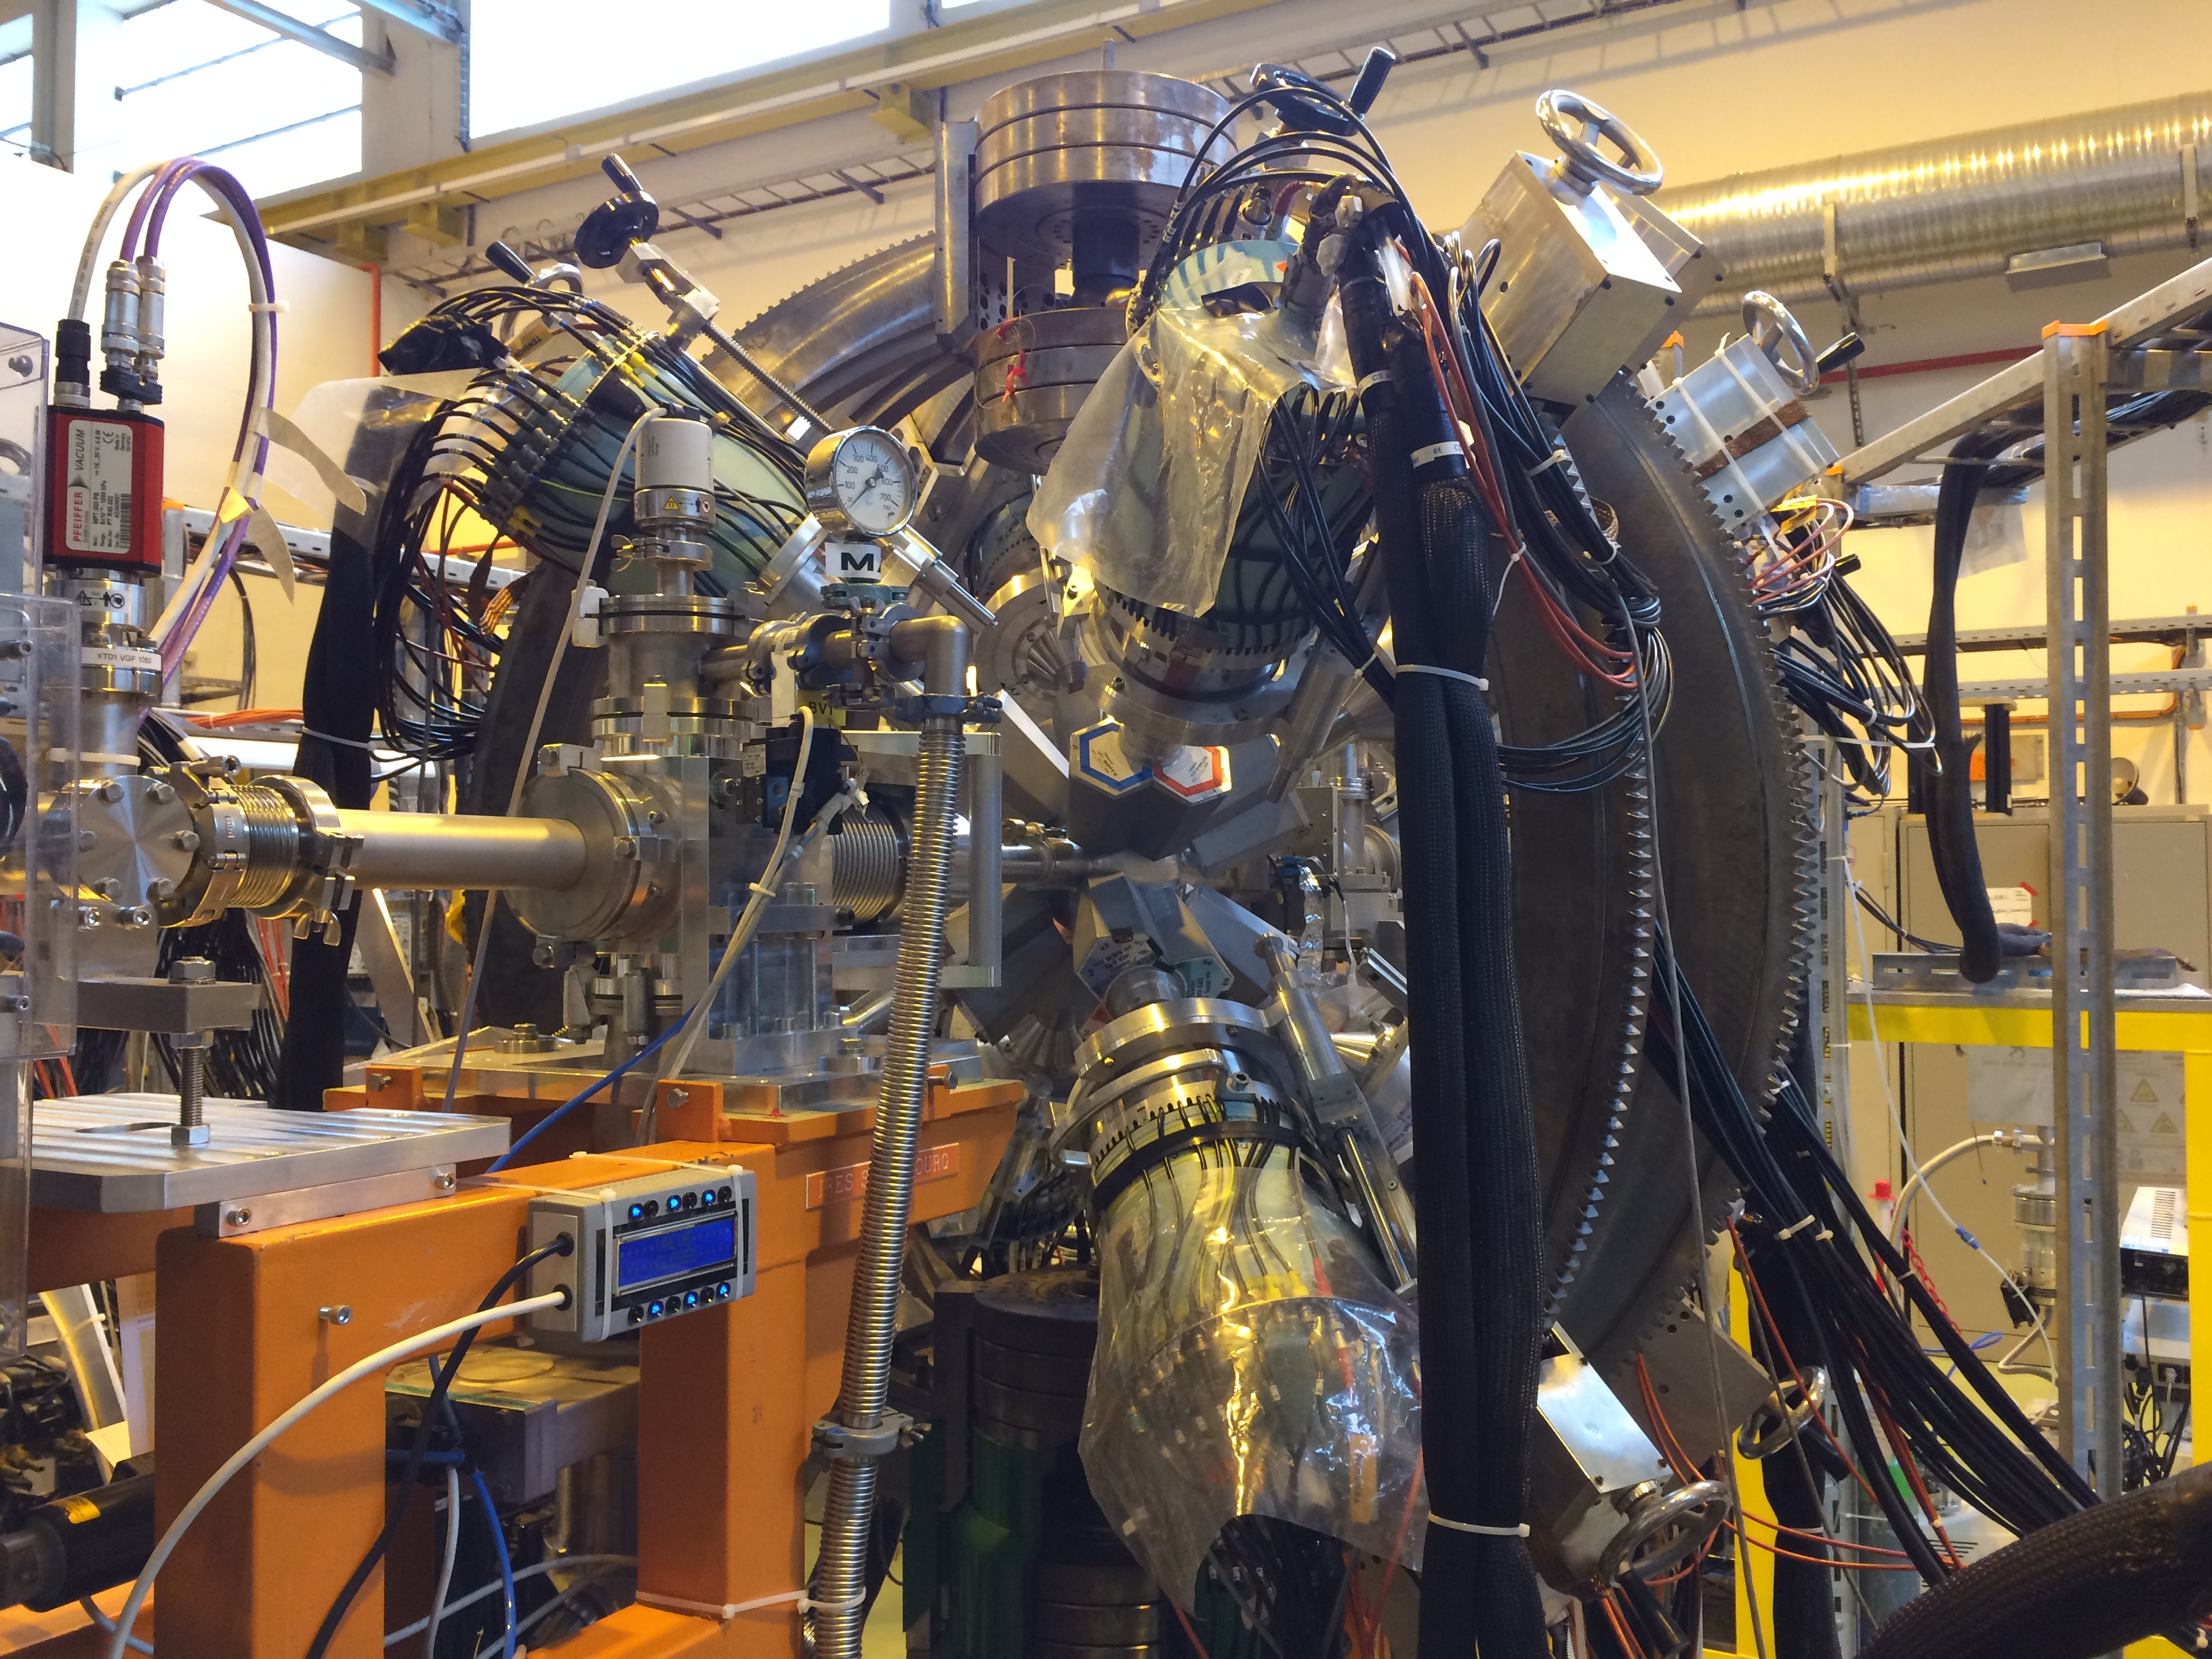
\includegraphics[width=\linewidth]{Images/IMG3849.JPG}
	\caption{Overview picture of the Miniball spectrometer. \\ Photo by: Trond Wiggo Johansen.}
	\label{fig:MBSpect}
\end{figure}


\subsubsection{Target chamber}
The target chamber is a hollow sphere made out of a machined out, single piece of aluminium alloy (AlMg$_3$), with a thin wall and an inner radius of approximately 80 mm. Inside the chamber we find a target wheel and a particle detector. The target wheel can hold up to six different targets as shown in \autoref{fig:TWheel}. The particle detector can be positioned 25 - 31 mm from the target wheel, limited by the space inside the chamber. Outside of the target chamber the average distance from each \ga-detector cluster to the center of the target chamber is approximately 10 cm. The forward detectors and the backward detectors has an angular position $\theta$ of approximately 45$^\circ$ and 135$^\circ$ respectively, compared to the beam line. In the vertical plane, perpendicular to the beam line, the four \ga-detectors in forward and backward position are placed roughly on a circle with a separation of $\phi = 90^\circ$ \cite{MB-spect}.  

\begin{figure}[ht]
	\centering
	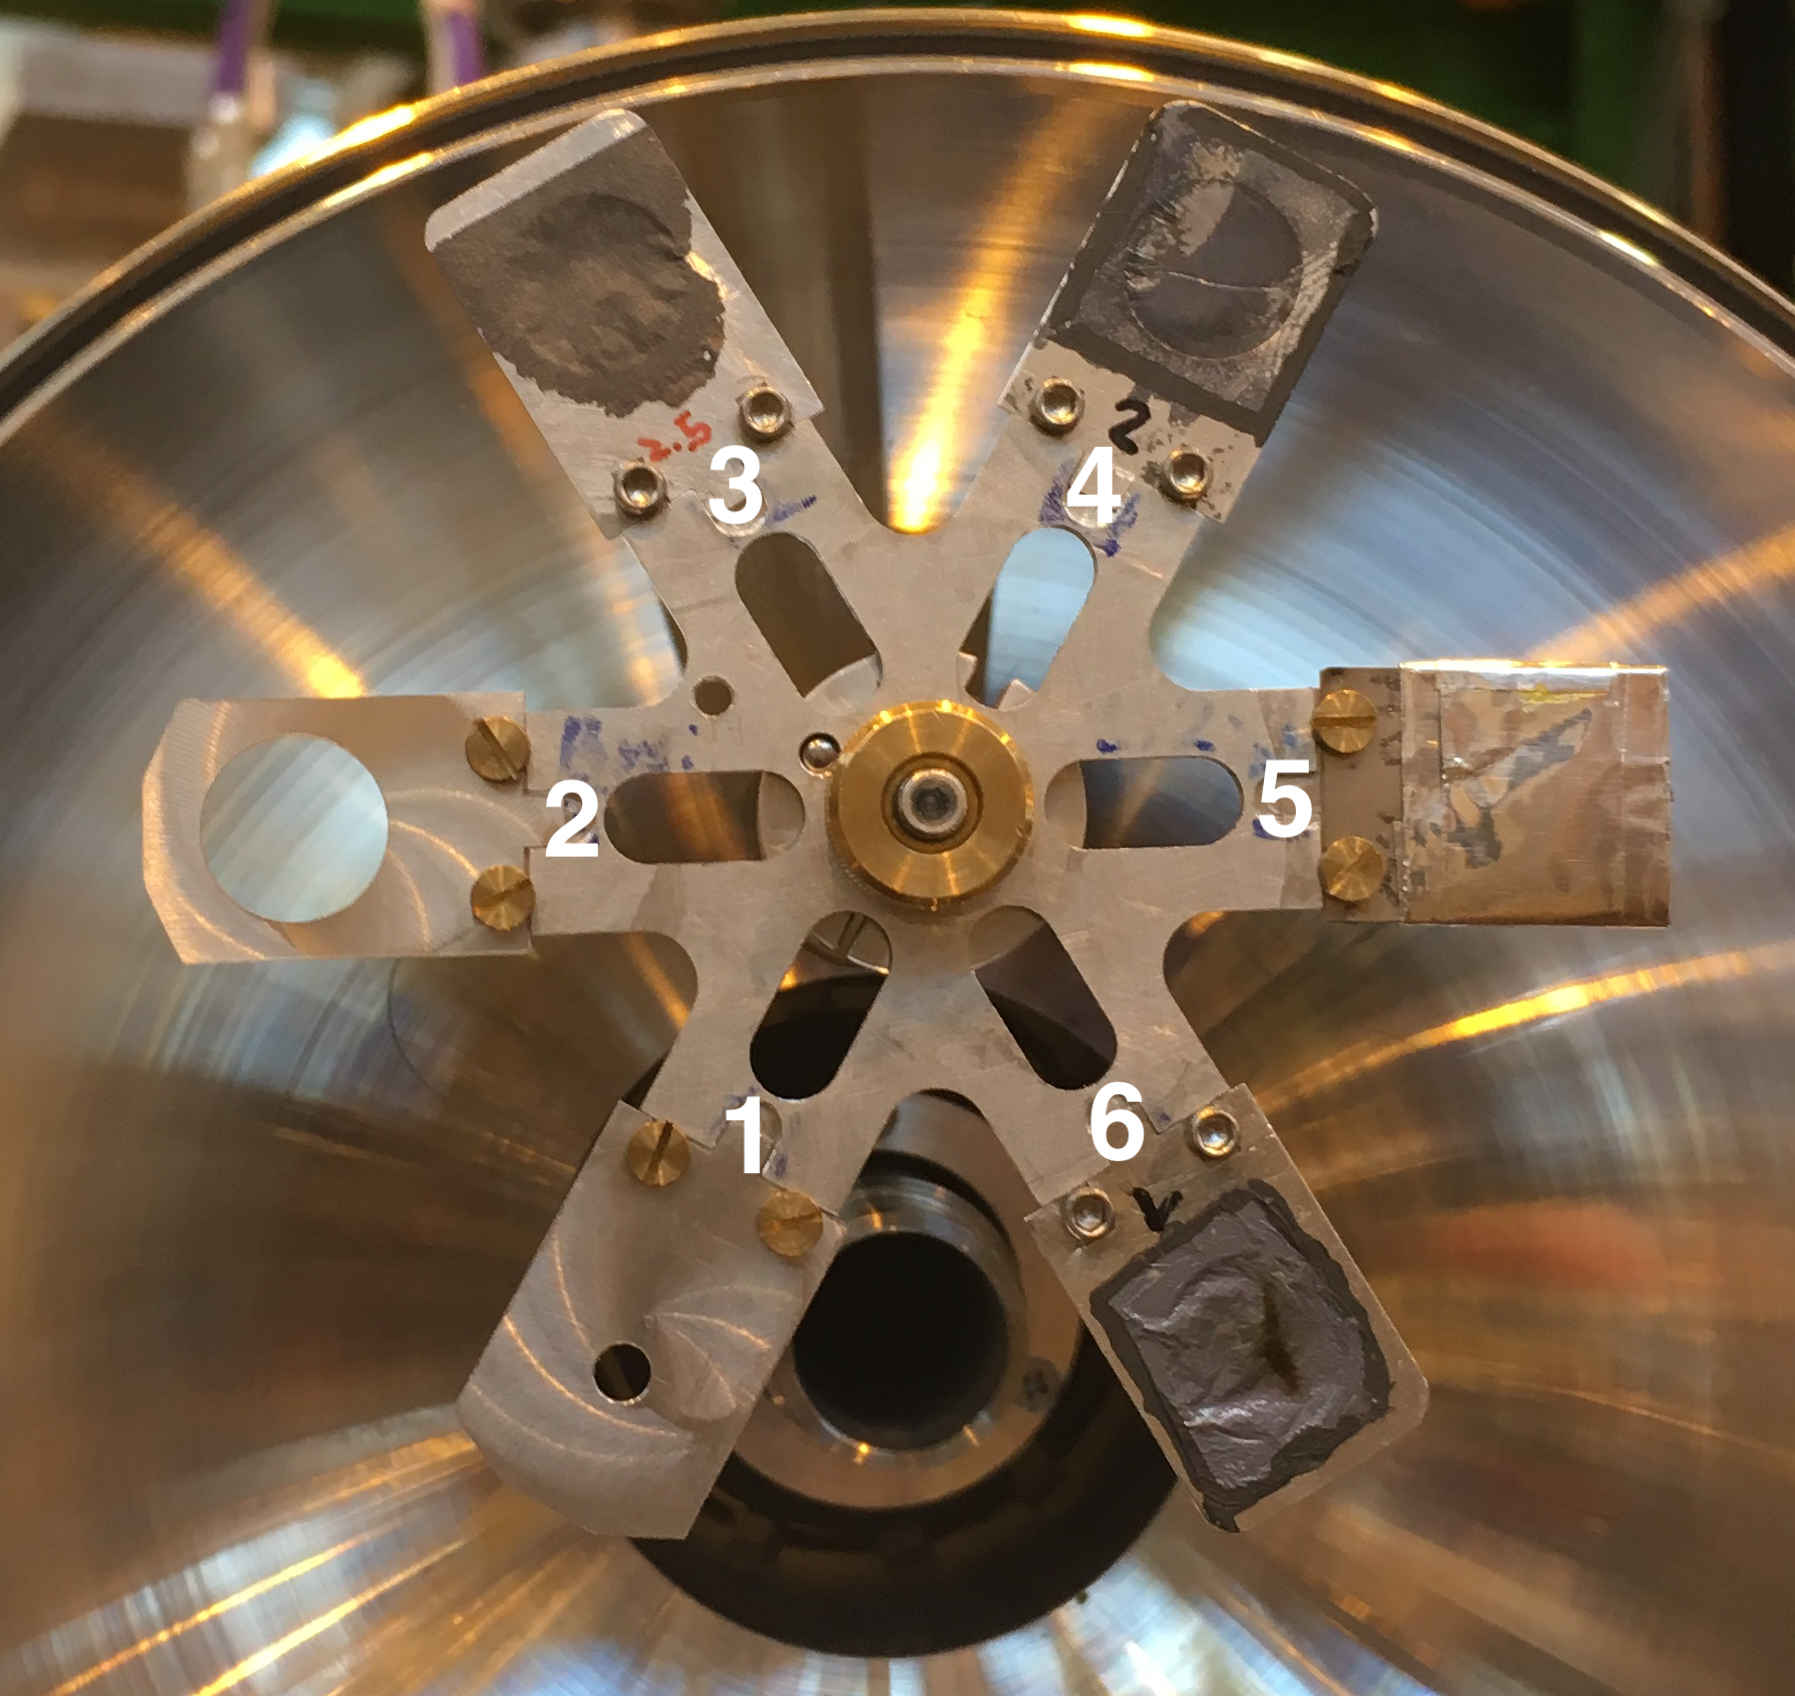
\includegraphics[width=\linewidth]{Images/Target-wheel.png}
	\caption{The target wheel can hold up to six different targets. Position 6 has the target \Pb\ with thickness 1.4 mg/cm$^2$. \\ Photo by: Dr. Liam Gaffney, date: 07.08.2017.}
	\label{fig:TWheel}
\end{figure}


\subsubsection{Particle detector, DSSSD (CD)}
To detect the scattered beam and target nuclei, a segmented Double Sided Silicon Strip Detector (DSSSD) composed of four quadrants was used. The DSSSD looks very like an audio Compact Disc (CD), and hence it is called the CD. In the front of the CD, one quadrant consists of 16 annular strips (rings) with a pitch of 2 mm, while the back consists of 24 sector (radial) strips with a pitch of 3.5$^\circ$. The innermost strip has an inner radius of the active area of 9 mm, while the outermost strip has an outer radius of the active area of 40.9 mm. There are in total 160 discrete detector elements for all four quadrants (64 in front, 96 in back). Each quadrant is connected to its own Analog to Digital Converter (ADC). Because of lack of available channels in the ADC, the sector strips in the back are paired up, so that it is effectively 12 sector strips in the back side. The CD detector has a total area of 5000 mm$^2$, where the active area is approximately 93$\%$. The silicon wafer thickness is between 50 $\mu$m and 1000 $\mu$m with a dead layer of 0.3 to 0.8 $\mu$m of aluminium. For simplicity the dead layer thickness is usually assumed to be 0.7 $\mu$m \cite{NWarr-CD, MB-spect}. \autoref{tab:CD_spec} shows some of the specifications of the CD and \autoref{fig:CD-FB} shows a sketch of the front and back side. 
The distance\footnote{The distance was measured using a $\alpha$-source ($^{226}$Ra). The source has a thickness of 1.23 mm, which needs to be factored in so that the target to CD distance is the CD to source distance plus the source thickness, that is 25.78(12) mm + 1.23 mm = 27.01 mm. This source data was reanalyzed since the original log entry, giving a 0.03 mm difference. From private communications at ISOLDE in August 2018, the distance from the target to the CD was determined to be 26.98 mm with a $\sim$1 mm uncertainty."} from the target to the CD was 26.98 mm ($\pm$ 1 mm). In the laboratory (LAB) reference frame the CD has a angular coverage between 18.4$^\circ$ and 56.6$^\circ$. An extensive description of the CD can be found in \cite{CD-DSSSD}.

\begin{table}[ht] 
    \centering 
    \caption{CD specifications.}
	% Data for the CD specification table
\begin{tabular}{lll}
\hline
                            & Annular strips & Secular strips \\
                            & (CD Front)     & (CD Back)      \\
\hline
Number of strips            & 16             & 24             \\
Inner radius of active area &  9.000 mm      & -              \\
Outer radius of active area & 40.900 mm      & -              \\
Strip pitch                 &  2.000 mm      & 3.5$^\circ$    \\
Strip width                 &  1.900 mm      & 3.4$^\circ$    \\
Strip length                &  -             & 31.900 mm      \\
Active angle coverage       & 81.6$^\circ$   & 81.6$^\circ$   \\
Inner strip distance        &  -             & 0.100 mm       \\
\hline
\end{tabular}
	\label{tab:CD_spec}
\end{table}


\begin{figure}[ht]
	\centering
	\begin{subfigure}{\textwidth}
		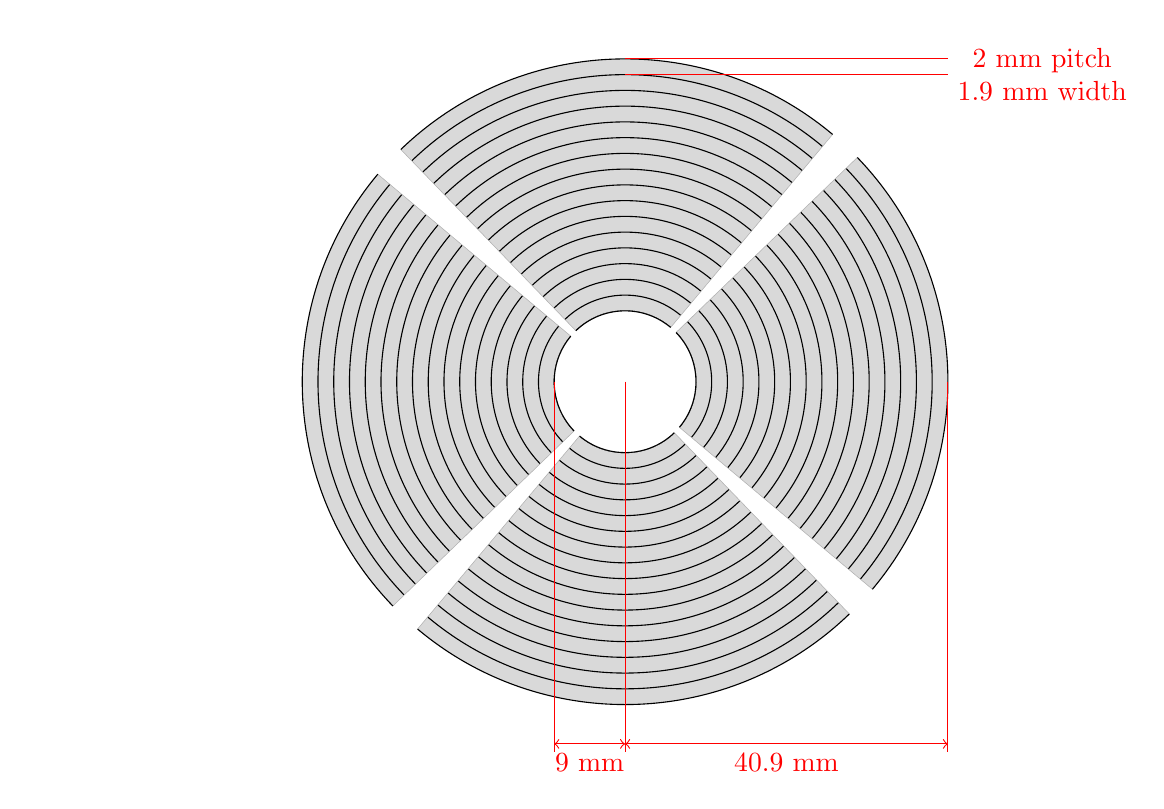
\begin{tikzpicture}
    % Definitions
    \coordinate (origo) at (0,0);
    \def \smallradius{0.9cm}
    \def \bigradius{4.1cm}
    \def \factor{0.2}
    \def \rotation{50}
    %%%
    %%% Front detector
    %%%
    % Gray background
    \foreach \factor in {0, 90, 180, 270} 
    {
        \fill[gray!30, rotate=\factor+\rotation] (origo) -- (\bigradius,0cm) arc (0:84:\bigradius) -- (origo);
    }
    % Annular lines
    \foreach \radius in {0.9, 1.1, ..., 4.1} 
    {
        \draw[black, rotate=\rotation, >=stealth]     (0:\radius) arc (0:84:\radius) {};
        \draw[black, rotate=90+\rotation, >=stealth]  (0:\radius) arc (0:84:\radius) {};
        \draw[black, rotate=180+\rotation, >=stealth] (0:\radius) arc (0:84:\radius) {};
        \draw[black, rotate=270+\rotation, >=stealth] (0:\radius) arc (0:84:\radius) {};
    }
    % Radial quadrant lines
    \foreach \x in {-6, 0, 84, 90, 174, 180, 264, 270} 
    {
        \draw[very thin, black!30, rotate=\rotation] (origo) -- (\x:\bigradius);
    }
    % Inner circle
    \draw[very thin, white, fill=white] (origo) circle (\smallradius);
    % Inner and outer circle arc
    \foreach \factor in {0, 90, 180, 270} 
    {
        \draw[black, rotate=\factor+\rotation, >=stealth] (0:\smallradius) arc (0:84:\smallradius) {};
        \draw[black, rotate=\factor+\rotation, >=stealth] (0:\bigradius) arc (0:84:\bigradius) {};
    }
    % Pitch/width
    \draw[red] (0,\bigradius) -- (\bigradius,\bigradius);
    \draw[red] (0,3.9) -- node[right, pos=1] {\shortstack{2 mm pitch \\ 1.9 mm width}} (\bigradius,3.9);
    % Inner/outer radius
    \draw[red] (-\smallradius,0) -- (-\smallradius,-4.7);
    \draw[red] (origo) -- (0,-4.7);
    \draw[red] (\bigradius, 0) -- (\bigradius,-4.7);
    \draw[<->, red] (-\smallradius,-4.6) -- node[below] {9 mm} (0,-4.6);
    \draw[<->, red] (0,-4.6) -- node[below] {40.9 mm} (\bigradius,-4.6);
    % Vertical alignment with back detector
    \node[] at (-7.47,0) {};
\end{tikzpicture}
		\caption{CD front: The numbering of the strips goes from strip 0 (outermost) to strip 15 (innermost). Quadrants are numbered in clockwise direction with respect to the beam direction, so that left is 1, up is 2, right is 3 and down is 4.}
		\label{fig:CD-F}
	\end{subfigure}
	\begin{subfigure}{\textwidth}
		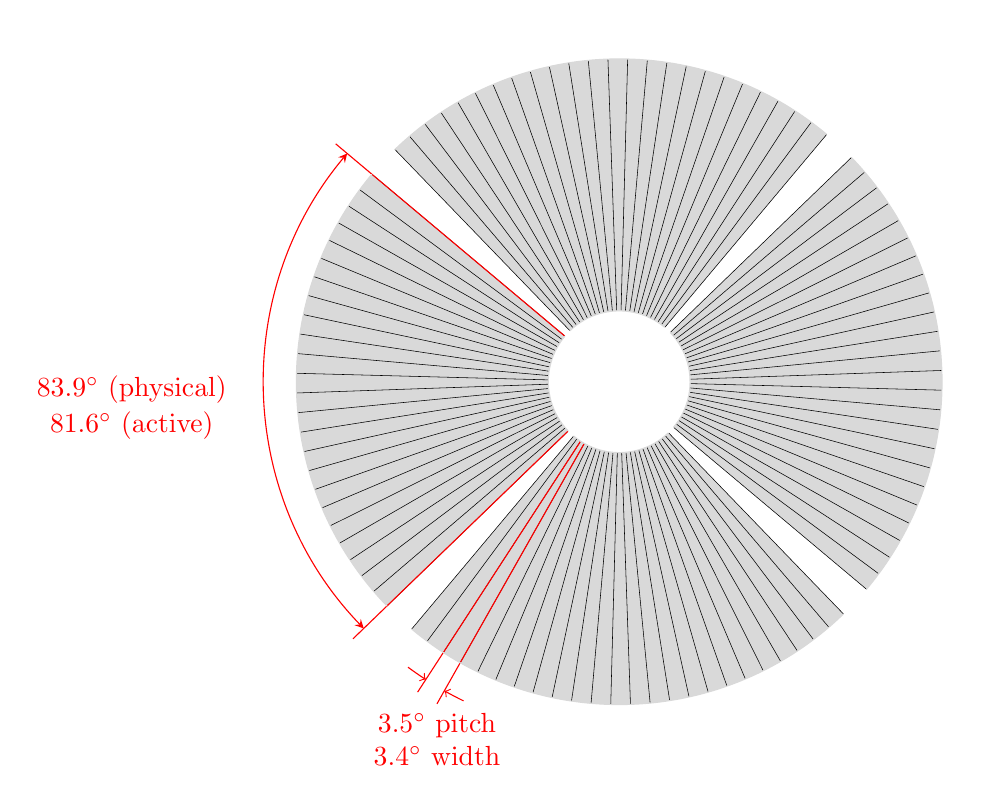
\begin{tikzpicture}
    % Definitions
    \coordinate (origo) at (0,0);
    \def \smallradius{0.9cm}
    \def \bigradius{4.1cm}
    \def \pitch{3.5}
    \def \rotation{50}
    %%%
    %%% Back detector
    %%%
    % Gray background
    \foreach \factor in {0, 90, 180, 270} 
    {
        \fill[gray!30, rotate=\factor+\rotation] (origo) -- (\bigradius,0cm) arc (0:84:\bigradius) -- (origo);
    }
    % Radial lines
    \foreach \x in {0, \pitch, ..., 84} 
    {
        \draw[very thin, black, rotate=\rotation]     (origo) -- (\x:\bigradius);
        \draw[very thin, black, rotate=90+\rotation]  (origo) -- (\x:\bigradius);
        \draw[very thin, black, rotate=180+\rotation] (origo) -- (\x:\bigradius);
        \draw[very thin, black, rotate=270+\rotation] (origo) -- (\x:\bigradius);
    }
    % Physical/active area
    \draw[red, rotate=90+\rotation] (origo) -- (4.7,0);
    \draw[red, rotate=174+\rotation] (origo) -- (4.7,0);
    \draw[<->, red, rotate=90+\rotation, >=stealth] (0:1.1*\bigradius) arc (0:84:1.1*\bigradius) node[anchor=south east, pos=0.7, outer sep=6mm] {\shortstack{$83.9^\circ$ (physical) \\ $81.6^\circ$ (active)}};
    % Pitch/width area
    \draw[red, rotate=187+\rotation] (origo) -- (4.7,0);
    \draw[red, rotate=190.5+\rotation] (origo) -- (4.7,0) node[anchor=north, pos=1] {\shortstack{$3.5^\circ$ pitch \\ $3.4^\circ$ width}};
    \draw[->, red, rotate=183.5+\rotation] (0:1.1*\bigradius) arc (0:\pitch:1.1*\bigradius) {};
    \draw[<-, red, rotate=190.5+\rotation] (0:1.1*\bigradius) arc (0:\pitch:1.1*\bigradius) {};
    % Inner circle
    \draw[very thin, white, fill=white] (origo) circle (\smallradius);
    % Inner and outer circle arc
    \foreach \factor in {0, 90, 180, 270} 
    {
        \draw[gray!30, rotate=\factor+\rotation] (0:\smallradius) arc (0:84:\smallradius) {};
        \draw[gray!30, rotate=\factor+\rotation] (0:\bigradius) arc (0:84:\bigradius) {};
    }
\end{tikzpicture}
		\caption{CD back: The numbering of the strips goes from strip 0 to strip 23 in counter-clockwise direction viewed from this side. Quadrants are numbered in clockwise direction with respect to the beam direction. From this perspective right is 1, up is 2, left is 3 and down is 4.}
		\label{fig:CD-B}
	\end{subfigure}
	\caption{CD sketch, adapted from \cite{NWarr-CD}.}
	\label{fig:CD-FB}
\end{figure}


\subsubsection{\texorpdfstring{$\gamma$}{Gamma} detectors, high-purity germanium (HPGe)}
In Coulomb excitation experiments the target chamber is surrounded by the \ga\ detectors as shown in \autoref{fig:MBSpectCU}. The \ga-ray spectrometer consists of a total of 24 six-fold segmented High-Purity Germanium (HPGe) crystals, which are divided into 8 clusters of 3 crystals each. Each crystal is encapsulated and segmented into 6 parts, making a total of 144 segments. For maximum efficiency, the detectors are placed in a compact geometry around the target chamber \cite{NWarr-HPGe, MB-spect}. The detector-array can cover a solid angle of about 60\% of 4$\pi$, when the optimum distance between the target chamber and the HPGe-clusters is achieved. The average energy resolution at $E_\gamma = 1.3$ MeV is 2.3 keV \cite{Butler2017}. From each detector we get seven signals in total for each event, one from the core and six from each segment. \textcolor{red}{This requires 168 channels for data aquisition.} The shapes of these signals is analyzed to get information of the position. Because of the segmentation of the detector, a better Doppler correction can be performed compared to using the whole crystal. During operation the HPGe-clusters needs to be cooled down by liquid nitrogen and there is an automated filling system in place for this \cite{NWarr-HPGe}. 

\begin{figure}[ht]
	\centering
	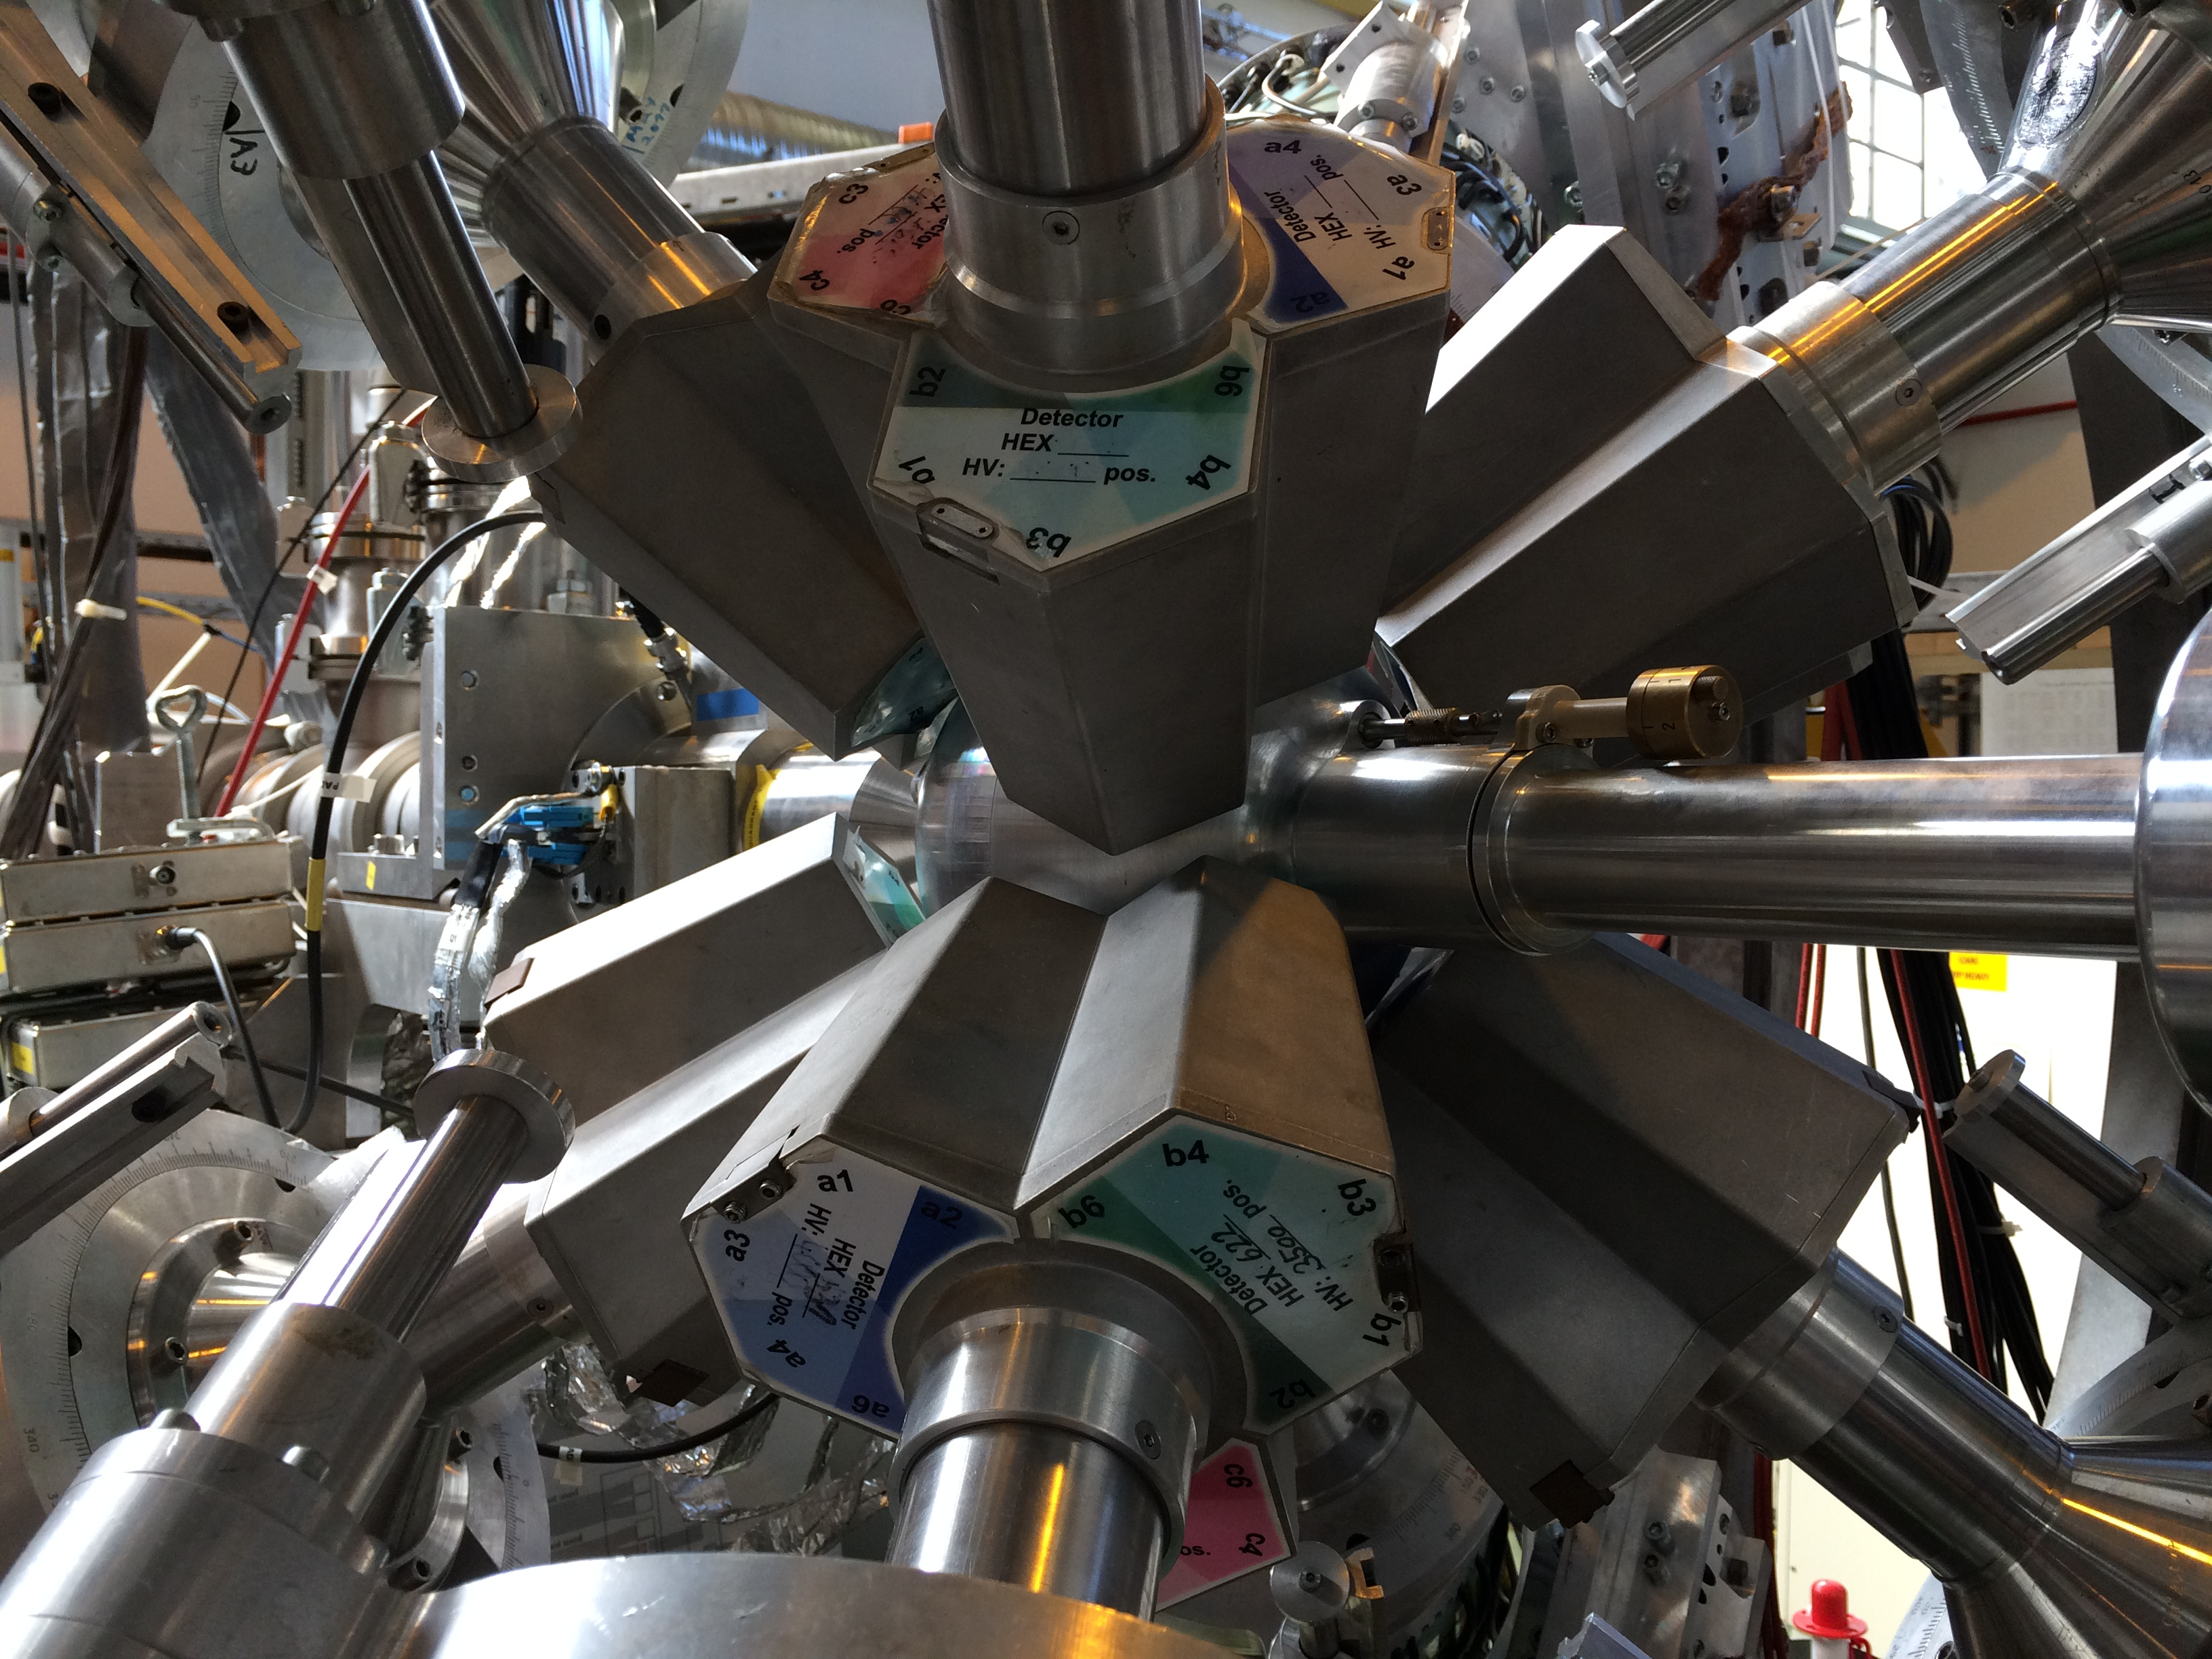
\includegraphics[width=\linewidth]{Images/IMG3917.JPG}
	\caption{Close up picture of the Miniball spectrometer. The Miniball target chamber is in the middle, surrounded by the triple-cluster encapsulated \ga\ crystals. The beam line goes through the target chamber. \\ Photo by: Trond Wiggo Johansen.}
	\label{fig:MBSpectCU}
\end{figure}


\section{Data acquisition system}
Signals from the CD and the HPGe clusters are read out by the ADC and Digital Gamma Finder (DGF) modules and sent to a Personal Computer (PC) in the Data AcQuisition (DAQ) room at ISOLDE where the data is then stored. The collection of data is done by the \MBOU\ \cite{Maraboou} DAQ system \cite{MB-spect}. It is split in two parts as shown in \autoref{fig:MARaBOOU}, one front-end part based on the Multi Branch System (MBS) \cite{MBS} and one back-end part based on the ROOT framework \cite{ROOT}. The front-end takes care of data readout, event building and data transportation, while the back-end takes care of the setup, run control, histogramming, data analysis and data storage. The system can manage high counting rates without dead time, where the limitation is essentially only pile-up. The ADCs and TDCs can buffer up to 32 events at a time \cite{MB-spect}. 


\begin{figure}[ht]
	\centering
	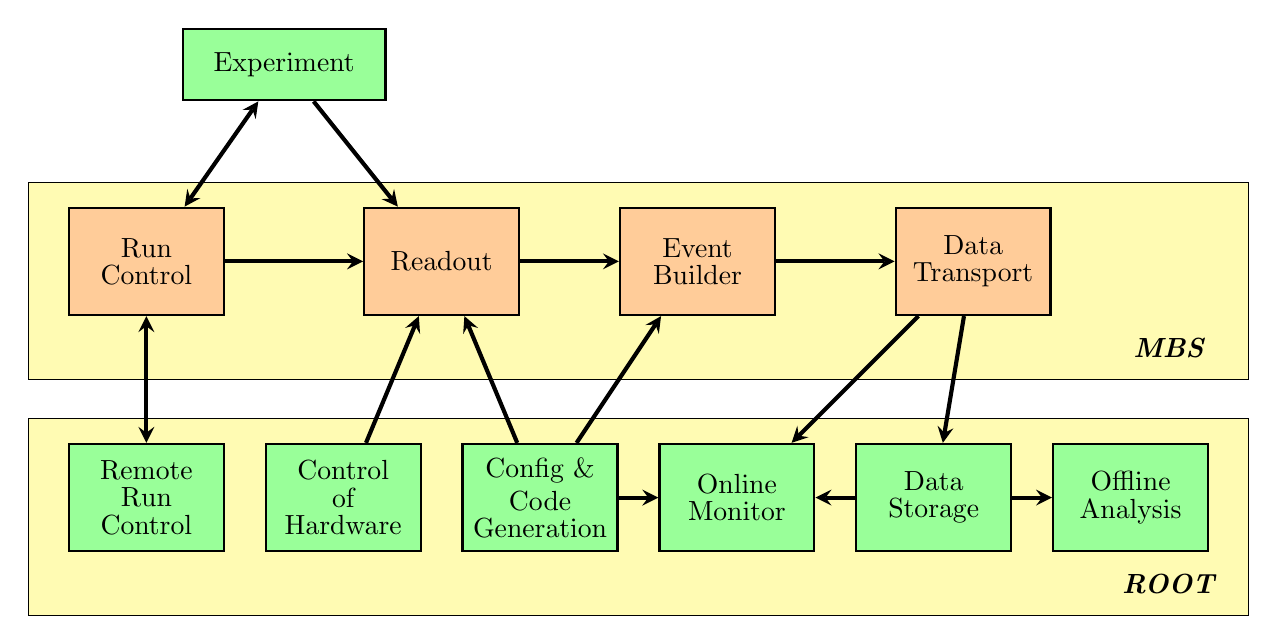
\begin{tikzpicture}
    % Definitions
    \coordinate (EX)  at (1.75,5.5);
    \coordinate (RC)  at (0,3);
    \coordinate (RO)  at (3.75,3);
    \coordinate (EB)  at (7,3);
    \coordinate (DT)  at (10.5,3);
    \coordinate (RRC) at (0,0);
    \coordinate (COH) at (2.5,0);
    \coordinate (CCG) at (5,0);
    \coordinate (OM)  at (7.5,0);
    \coordinate (DS)  at (10,0);
    \coordinate (OA)  at (12.5,0);
    % Rectangles
    \draw[fill=yellow!30] (-1.5,1.5)  rectangle (14,4);
    \draw[fill=yellow!30] (-1.5,-1.5) rectangle (14,1);
    % Nodes
    \node(Expe)   at (EX)  [draw,thick,minimum width=+17ex,minimum height=+6ex,fill=green!40]  {Experiment}; 
    \node(RuCo)   at (RC)  [draw,thick,minimum width=+13ex,minimum height=+9ex,fill=orange!40] {\shortstack{Run \\ Control}};
    \node(ReOu)   at (RO)  [draw,thick,minimum width=+13ex,minimum height=+9ex,fill=orange!40] {Readout};
    \node(EvBu)   at (EB)  [draw,thick,minimum width=+13ex,minimum height=+9ex,fill=orange!40] {\shortstack{Event \\ Builder}};
    \node(DaTr)   at (DT)  [draw,thick,minimum width=+13ex,minimum height=+9ex,fill=orange!40] {\shortstack{Data \\ Transport}};
    \node(ReRuCo) at (RRC) [draw,thick,minimum width=+13ex,minimum height=+9ex,fill=green!40]  {\shortstack{Remote \\ Run \\ Control}};
    \node(CoofHa) at (COH) [draw,thick,minimum width=+13ex,minimum height=+9ex,fill=green!40]  {\shortstack{Control \\ of \\ Hardware}};
    \node(CoCoGe) at (CCG) [draw,thick,minimum width=+13ex,minimum height=+9ex,fill=green!40]  {\shortstack{Config \& \\ Code \\ Generation}};
    \node(OnMo)   at (OM)  [draw,thick,minimum width=+13ex,minimum height=+9ex,fill=green!40]  {\shortstack{Online \\ Monitor}};
    \node(DaSt)   at (DS)  [draw,thick,minimum width=+13ex,minimum height=+9ex,fill=green!40]  {\shortstack{Data \\ Storage}};
    \node(OfAn)   at (OA)  [draw,thick,minimum width=+13ex,minimum height=+9ex,fill=green!40]  {\shortstack{Offline \\ Analysis}};
    \node[thick] at (13,1.9)  {$\textbf{\textit{MBS}}$};
    \node[thick] at (13,-1.1) {$\textbf{\textit{ROOT}}$};
    % Arrows
    \draw[<->,>=stealth,line width=1.5pt] (Expe)   -- (RuCo);
    \draw[->,>=stealth,line width=1.5pt]  (Expe)   -- (ReOu);
    \draw[->,>=stealth,line width=1.5pt]  (RuCo)   -- (ReOu);
    \draw[->,>=stealth,line width=1.5pt]  (ReOu)   -- (EvBu);
    \draw[->,>=stealth,line width=1.5pt]  (EvBu)   -- (DaTr);
    \draw[->,>=stealth,line width=1.5pt]  (DaTr)   -- (OnMo);
    \draw[->,>=stealth,line width=1.5pt]  (DaTr)   -- (DaSt);
    \draw[<->,>=stealth,line width=1.5pt] (RuCo)   -- (ReRuCo);
    \draw[->,>=stealth,line width=1.5pt]  (CoofHa) -- (ReOu);
    \draw[->,>=stealth,line width=1.5pt]  (CoCoGe) -- (ReOu);
    \draw[->,>=stealth,line width=1.5pt]  (CoCoGe) -- (EvBu);
    \draw[->,>=stealth,line width=1.5pt]  (CoCoGe) -- (OnMo);
    \draw[->,>=stealth,line width=1.5pt]  (DaSt)   -- (OnMo);
    \draw[->,>=stealth,line width=1.5pt]  (DaSt)   -- (OfAn);
\end{tikzpicture}
	\caption{\protect\MBOU\ tasks, adapted from \cite{Maraboou}.}
	\label{fig:MARaBOOU}
\end{figure}


% ----------------------------------------------------------------------------------------------------------------------% ----------------------------------------------------------------------------------------------------------------------


\chapter{Data analysis}  

In this chapter, the various programs and scripts applied in the detector calibration and data analysis will be introduced. 
Scripts developed in the present thesis work for the fitting procedures are slightly based on scripts written by Ville Virtanen\footnote{Ville Virtanen is a student from University of Jyväskylä.} and Dr. Liam Gaffney\footnote{Dr. Liam Gaffney is a research fellow at ISOLDE, affiliated with Miniball.}. 
The codes have been further developed and heavily re-written in the current work. 
Presently the code has only a minor resemblance to the original code. 
The remaining Python and bash scripts are written and developed by the author.
All of the scripts written in C/C++ are dependent on the ROOT framework, a C/C++ data analysis framework developed and maintained at CERN.


\section{Data handling}
The raw data from Miniball experiments essentially\footnote{The format is not entirely correct, since it has identification of where the particle and \ga\ hit. 
A more detailed format is: identification, time, particle energy (front strip, back strip), \ga\ energy (cluster, crystal, segment), etc.} comes in list mode (identification, energy, time), where every line is an event. 
It is stored in \textit{.med}-files, MBS Event Data or also known as Miniball Event Data, with the naming convention \textit{140Sm\_208Pb\_pos6\_0xy.med} for this experiment, where \textit{x} and \textit{y} are numbers between 0 and 9. 
The goal of the data analysis is to obtain Doppler-corrected \ga-spectra with various conditions on particles and angles, in order to analyze the Coulomb excitation of \Sm. 

%\begin{lstlisting}[language=]
%$ cd ~/GitHub/MasterThesis/Raw_data/Sm
%$ root 140Sm_208Pb_pos6_008_OnBeam.root
%root [1] tr->Show(10)
%======> EVENT:10
% Event           = (BuiltEvent*)0x7f8db0469010
% fUniqueID       = 0
% fBits           = 33554432
% ebisTime        = 16936792
% t1Time          = 0
% superCycleTime  = 65948
% eventNumber     = 100
% subEventNumber  = 12
% dgfData         = (vector<DgfData>*)0x7f8db04690c0
% dgfData.fUniqueID = 0
% dgfData.fBits   = 33554432
% dgfData.fModuleNumber = 18
% dgfData.fChannel = 0
% dgfData.fMultiplicity = 1
% dgfData.fEventTime = 40774
% dgfData.fEnergy = 583
% dgfData.fFastTriggerTime = 40799
% dgfData.fLongFastTriggerTime = 16949087
% dgfData.fUserValues[6] = 26112 , 60811 , 32766 , 0 , 38240 , 60811
%\end{lstlisting}

For Miniball experiment data, the preferred sorting and analysis code is \textsl{MiniballCoulexSort} \cite{MBCS}. 
The main steps of how to download, install\footnote{If the \textbf{make} step fails, try doing a \textbf{make clean} and then \textbf{make}. The program might think that it is already built.} and use it is outlined in the \textit{README.md} file in the GitHub repository of Miniball, linked in the reference. 
The program is written in C/C++ and depends on the ROOT framework. 
It is under constant development at CERN-ISOLDE under the management of Dr. Liam Gaffney. 
Unfortunately the code isn't very well documented, so it takes some time to learn what it does and how to use it. 
To get from the raw data to the Doppler-corrected \ga-spectra, the code is divided into a three step procedure:

\begin{enumerate}
	\item \texttt{MedToRoot}
	\begin{itemize}
		\item converts the raw data to ROOT format
	\end{itemize}
	\item \texttt{TreeBuilder}
	\begin{itemize}
		\item event building
		\begin{itemize}
			\item calibrate detectors and apply thresholds
			\item use particle-\ga\ coincidences (correlations) to build events
			\item store everything in a three structure for easy access
		\end{itemize}
	\end{itemize}
	\item \texttt{CLXAna}
	\begin{itemize}
		\item apply gates on particles and perform Doppler correction
	\end{itemize}
\end{enumerate}

For the CD, \texttt{TreeBuilder}\footnote{\texttt{TreeBuilder} is found in the \textit{$\sim$/GitHub/Miniball/MiniballCoulexSort/TreeBuilder} directory.} sorts each quadrant for itself, but it is not possible to see each pixel of the detector. 
In the front, each annular strip can be viewed and in the back each secular strip can be viewed as a whole, the back strip contains the energy information of all of the 16 annular strips. 
The secular strips cover a wide angular range, thus they show no sharp peaks.
\texttt{TreeBuilder} also takes a number of command line flag options. 
If the \textit{-cdpad} flag option is not used, then there will be no particle events, because they come into the CD. 
Other flag options will be introduced later in the chapter.

One program that is mentioned in the Miniball GitHub repository, but not showed how to use, is the \texttt{AQ4Sort}\footnote{\texttt{AQ4Sort} is also found in the \textit{$\sim$/GitHub/Miniball/MiniballCoulexSort/TreeBuilder} directory.}. 
It is used in the same way as the \texttt{TreeBuilder} script, but it sorts the histograms in another way and it does not take any command line flag options. 
\texttt{AQ4Sort} is used before and during the calibration of the particle detectors, because it gives information about every single ring and every single back strip (the "pixels" of the CD). 
These pixels are used for calibration and are made by gating on the annular (front) rings to see peaks in the secular (back) strips. 


\subsection{Counting and naming convention}
The numbering of the CD rings and strips are different in different programs and scripts. 
Histograms sorted by \texttt{TreeBuilder} starts counting from 0 (outermost ring) to 15 (innermost ring) as showed in \autoref{fig:CD-FB}. 
\texttt{AQ4Sort} starts from 1 (outermost ring) to 16 (innermost ring), shifted compared to \texttt{TreeBuilder}.
For calibrated spectra, \texttt{TreeBuilder} shows the energy in MeV, while \texttt{AQ4Sort} shows energy in keV.
The simulation program \texttt{kinsim3} counts from 1 (innermost ring) to 16 (outermost ring), the opposite of \texttt{AQ4Sort}. 
It is easy to be confused by all the different counting, but this thesis will try to use the counting order of \texttt{kinsim3} for the CD, it seems like the most logic way of counting. 
\autoref{tab:ADC} shows the CD wiring.
A change of the wiring of the CD will probably not happen, but it is possible to choose a logic order of counting software wise.
\autoref{tab:TBvsAQ4} shows a comparison of the logic counting and the histogram naming from \texttt{TreeBuilder} and \texttt{AQ4Sort}.
Calibration coefficients given to the calibration file, which is introduced in later sections, follow the naming convention of \texttt{TreeBuilder} in \autoref{tab:TBvsAQ4}.


\begin{table}[ht] 
	\centering 
	\caption{CD wiring for Coulomb excitation experiments.}
	% Data for the ADC table
\caption{ADC}
\label{tab:ADC}
\begin{tabular}{cccc}
\hline
ADC    & Quadrant & Channel &  \shortstack{Front ring [F] or \\ back strip [B]} \\
\hline
0 - 3  &  1 - 4   &  0      &  F                    		   					\\
0 - 3  &  1 - 4   &  1      &  F                    		   					\\
0 - 3  &  1 - 4   &  2      &  F                    		   					\\
0 - 3  &  1 - 4   &  3      &  F                    		   					\\
0 - 3  &  1 - 4   &  4      &  F                    		   					\\
0 - 3  &  1 - 4   &  5      &  F                    		   					\\
0 - 3  &  1 - 4   &  6      &  F                    		   					\\
0 - 3  &  1 - 4   &  7      &  F                    		   					\\
0 - 3  &  1 - 4   &  8      &  F                    		   					\\
0 - 3  &  1 - 4   &  9      &  F                    		   					\\
0 - 3  &  1 - 4   &  10     &  F                    		   					\\
0 - 3  &  1 - 4   &  11     &  F                    		   					\\
0 - 3  &  1 - 4   &  12     &  F                    		   					\\
0 - 3  &  1 - 4   &  13     &  F                    		   					\\
0 - 3  &  1 - 4   &  14     &  F                    		   					\\
0 - 3  &  1 - 4   &  15     &  F                    		   					\\
0 - 3  &  1 - 4   &  16     &  B                    		   					\\
0 - 3  &  1 - 4   &  17     &  B                    		   					\\
0 - 3  &  1 - 4   &  18     &  B                    		   					\\
0 - 3  &  1 - 4   &  19     &  B                    		   					\\
0 - 3  &  1 - 4   &  20     &  B                    		   					\\
0 - 3  &  1 - 4   &  21     &  B                    		   					\\
0 - 3  &  1 - 4   &  22     &  B                    		   					\\
0 - 3  &  1 - 4   &  23     &  B                    		   					\\
0 - 3  &  1 - 4   &  24     &  B                    		   					\\
0 - 3  &  1 - 4   &  25     &  B                    		   					\\
0 - 3  &  1 - 4   &  26     &  B                    		   					\\
0 - 3  &  1 - 4   &  27     &  B                    		   					\\
0 - 3  &          &  28     &  Empty                		   					\\
0 - 3  &          &  29     &  Empty                		   					\\
0 - 3  &          &  30     &  Empty                		   					\\
0 - 3  &  1 - 4   &  31     &  PAD                  		   					\\
  4    &          &  0      &  Ionization Chamber   		   					\\
  4    &          &  1      &  Ionization Chamber   		   					\\
\hline
\end{tabular}

	\label{tab:ADC}
\end{table}


\begin{table}[ht] 
	\centering 
	\caption{The logic counting and the naming of histograms from \texttt{TreeBuilder} and \texttt{AQ4Sort}.}
	% Data for the TreeBuilder vs AQ4Sort table
\caption{TreeBuilder vs AQ4Sort.}
\label{tab:TBvsAQ4}
\begin{tabular}{cccc}
\hline
Quadrant  &  Front ring or back strip  &  TreeBuilder  &  AQ4Sort      \\
\hline
1         &  Front ring 15             &  adc\_0\_0    &  fE\_Q1\_f1   \\
1         &  Front ring 14             &  adc\_0\_1    &  fE\_Q1\_f2   \\
1         &  Front ring 13             &  adc\_0\_2    &  fE\_Q1\_f3   \\
$\vdots$  &  $\vdots$                  &  $\vdots$     &  $\vdots$     \\
1         &  Front ring 1              &  adc\_0\_14   &  fE\_Q1\_f15  \\
1         &  Front ring 0              &  adc\_0\_15   &  fE\_Q1\_f16  \\
1         &  Back strip 0              &  adc\_0\_16   &  bE\_Q1\_f1   \\
1         &  Back strip 1              &  adc\_0\_17   &  bE\_Q1\_f2   \\
1         &  Back strip 2              &  adc\_0\_18   &  bE\_Q1\_f3   \\
$\vdots$  &  $\vdots$                  &  $\vdots$     &  $\vdots$     \\
1         &  Back strip 11             &  adc\_0\_26   &  bE\_Q1\_f11  \\
1         &  Back strip 12             &  adc\_0\_27   &  bE\_Q1\_f12  \\
          &                            &               &               \\
2         &  Front ring 15             &  adc\_1\_0    &  fE\_Q2\_f1   \\
$\vdots$  &  $\vdots$                  &  $\vdots$     &  $\vdots$     \\
2         &  Front ring 0              &  adc\_1\_15   &  fE\_Q2\_f16  \\
2         &  Back strip 0              &  adc\_1\_16   &  bE\_Q2\_f1   \\
$\vdots$  &  $\vdots$                  &  $\vdots$     &  $\vdots$     \\
2         &  Back strip 12             &  adc\_1\_27   &  bE\_Q2\_f12  \\
          &                            &               &               \\
3         &  Front ring 15             &  adc\_2\_0    &  fE\_Q3\_f1   \\
$\vdots$  &  $\vdots$                  &  $\vdots$     &  $\vdots$     \\
3         &  Front ring 0              &  adc\_2\_15   &  fE\_Q3\_f16  \\
3         &  Back strip 0              &  adc\_2\_16   &  bE\_Q3\_f1   \\
$\vdots$  &  $\vdots$                  &  $\vdots$     &  $\vdots$     \\
3         &  Back strip 12             &  adc\_2\_27   &  bE\_Q3\_f12  \\
          &                            &               &               \\
4         &  Front ring 15             &  adc\_3\_0    &  fE\_Q4\_f1   \\
$\vdots$  &  $\vdots$                  &  $\vdots$     &  $\vdots$     \\
4         &  Front ring 0              &  adc\_3\_15   &  fE\_Q4\_f16  \\
4         &  Back strip 0              &  adc\_3\_16   &  bE\_Q4\_f1   \\
$\vdots$  &  $\vdots$                  &  $\vdots$     &  $\vdots$     \\
4         &  Back strip 12             &  adc\_3\_27   &  bE\_Q4\_f12  \\
\hline
\end{tabular}
	\label{tab:TBvsAQ4}
\end{table}


\section{Data conversion}
In order to analyze the data in the ROOT framework, the first part of the code is just to convert the \textit{.med}-files produced by \MBOU\ into \textit{.root}-files with the program \texttt{MedToRoot}. 
To avoid copy and paste the commands used with \texttt{MedToRoot} in the terminal for every data file, a bash script called \texttt{M2R.sh} was made to do this. 
It uses \texttt{MedToRoot} to take in as many files as you want, and convert it in one go. 
It takes one command line argument because it was initially developed to convert files from different elements, so it is fairly simple to expand. 
If no command line arguments are given, the script will print out how to use it.
First all of the interesting raw data files are converted with the \texttt{M2R.sh} script. 
An example of the use with terminal output for the \textit{140Sm\_208Pb\_pos6\_0xy.med}-file with \textit{xy = 08} is as follows:

% Empty language = plain text
\begin{lstlisting}[language=]
$ cd ~/GitHub/MasterThesis/Scripts/sorting
$ ./M2R.sh Sm
opening file ../../Raw_data/Sm/140Sm_208Pb_pos6_008.med ...
EventBuffer::EventBuffer(GlobalSettings *)
Processing event number       0
Start trigger #14

Processing event number  130000
Stop trigger #15


Unpacked 132802 events:
wrong dgf hit pattern:                      0 ( 0.0 %)
wrong adc headers:                          0 ( 0.0 %)
# of overflows in adc channels:        599712 (451.6 %)
# of underflows in adc channels:            0 ( 0.0 %)
pattern unit mismatches:                    0 ( 0.0 %)

Number of ebis pulses:            66351
Number of t1 pulses:               2211
Number of supercycle pulses:        429
committed       1 243 951 987  bytes to tree tr, 'Tree for on beam data of Coulex setup@Miniball'
and                15 338 250  bytes to tree bg, 'Tree for on beam background data of Coulex setup@Miniball'
and               237 454 436  bytes to tree tr, 'Tree for off beam data of Coulex setup@Miniball'
wrote                  97 189  bytes to file ../../Raw_data/Sm/140Sm_208Pb_pos6_008_OnBeam.root 	=> compressed by a factor of 12799.3
,                      18 362  bytes to file ../../Raw_data/Sm/140Sm_208Pb_pos6_008_OnBeamBackground.root 	=> compressed by a factor of 835.3
,                      67 934  bytes to file ../../Raw_data/Sm/140Sm_208Pb_pos6_008_OffBeam.root 	=> compressed by a factor of 3495.4
and                    22 167  bytes to file ../../Raw_data/Sm/140Sm_208Pb_pos6_008_Scaler.root 	=> compressed by a factor of 2769.1
\end{lstlisting}

For each file converted with \texttt{MedToRoot}, the program makes four files with the naming convention
\begin{itemize}
	\item \textit{140Sm\_208Pb\_pos6\_0xy\_OnBeam.root} 
	\item \textit{140Sm\_208Pb\_pos6\_0xy\_OnBeamBackground.root}
	\item \textit{140Sm\_208Pb\_pos6\_0xy\_OffBeam.root}
	\item \textit{140Sm\_208Pb\_pos6\_0xy\_Scaler.root} 
\end{itemize}
where the file of interest is the first one. The \textit{OnBeam.root}-files are the files used in the sorting and event building with \texttt{TreeBuilder} and/or \texttt{AQ4Sort}.


\section{Detector calibration}


\textcolor{Magenta}{Tilbakemelding: \newline 
start with explaining the general idea for the calibration: \newline 
determine centroids of peaks in spectra, compare with simulations (kinematics, energy loss) to get linear coefficients (gain + offset). You could show spectra for 2 rings: one where it is ok to get the 2 centroids for Sm and Pb, and one where it is difficult $\rightarrow$ use additional data (Ni?) \newline
Sectors: cover wide angular range $\rightarrow$ no sharp peaks  \newline
Solution: gate on rings to see peaks in sectors and calibrate. \newline
Idea: \newline
1. produce spectra \newline
2. set thresholds: example, explain criteria \newline
3. find calibration coefficients $\rightarrow$ see above \newline
explain strategy, show examples... \newline
4. time calibration 
} \newline

\textcolor{Magenta}{ 
if you try to write this step-by-step cook book, you could introduce your scripts wherever is the right place to use them. 
}\newline

The general idea of the calibration is to make sure that the energy spectra from the detectors have the same physical features, that the detectors show the same energy distribution at the same position for the same kind of particles or \ga-rays hitting the same or the angular similarly place in the detectors.
Calibration of the detectors minimize the measurement uncertainty by making the detectors more accurate and consistent.
We want to determine centroids of peaks in the spectra, compare these with simulations using kinematics of the reaction and energy loss, to get linear coefficients of the detectors. 

Both detector types in this experiment are semiconductor detectors. 
Except for silicon (as the CD), semiconductors generally require cooling to low temperatures before they can be operated. 
The basic principle of operation is that incoming ionizing radiation\footnote{For the CD, the ionizing radiation is the beam or target particles scattered from the reaction, while the ionizing radiation for the HPGe-detectors is the high-energy photons (\ga) from de-excitation of the nuclei.} creates electron-hole pairs in the semi-conducting material which are then collected by an electric field. 
The number of electron-hole pairs is proportional to the energy of the incoming radiation to the semiconductor \cite{WRLeo}. 

Assuming a linear correlation between the energy $E$ of the particle (or \ga-ray) and the channel number $n$ of the ADC (or DGF), we get
\begin{equation}\label{eq:Ego}
	E = g \cdot n + a
\end{equation}
where $a$ is the offset in keV and $g$ is the gain in keV/$n$. 
The gain $g$ and the offset $a$ are the coefficients needed to do the calibration.
From \autoref{eq:Ego}, the offset $a$ can easily be expressed as 
\begin{equation}\label{eq:offset}
	a = E - g \cdot n 
\end{equation}
To find the gain $g$ in the CD denoted by $p$ for particle (or \ga-detectors denoted by \ga), at least two measuring points are needed, e.g. the peak energy of Sm and the peak energy of Pb for a given angle (or the peak of Eu and Ba explained in  \autoref{sec:gamma}). 
The relationship can be written as 
\begin{align}\label{eq:gain}
	g_p &= \frac{E_{\text{Sm}} - E_{\text{Pb}}}{n_{\text{Sm}} - n_{\text{Pb}}}
	&
	\Bigg( g_\gamma &= \frac{E_{\text{Eu}} - E_{\text{Ba}}}{n_{\text{Eu}} - n_{\text{Ba}}} \Bigg)
\end{align}
where the peak energies are obtained from a simulation of the Coulomb excitation experiment and the channel numbers are obtained from the raw data of the actual experiment.

On the front side of the CD we only have two measuring points per angle interval\footnote{Not entirely true, since we have three peaks in the spectra. But since we don't know what the contaminant is, we effectively only have two known measuring points.}, while on the back side of the CD we have we have two peaks per gated annular strip that we can fit. 
By doing a function fit (Gaussian or other), we can get the centroids (channels of the maximum or center of the peaks) for both Sm and Pb. 
For more than two centroids per strip, as the back side of the CD have, linear regression is used to find the best fit of the calibration coefficients.

An assumption when calibrating is that the energy on the front side and the back side of the detector is the same. 
This is not entirely correct, since there will be a small energy loss when the particle goes through the front side, but in most cases this is negligible.
Calibrating the back strips of the CD is the same as the front, however because they cover a large range of angles in the $\theta$ direction (according to \autoref{fig:LAB}), a gate on one of the front strips is needed to define an angle and thereby an energy. 
For this purpose, the program \texttt{AQ4Sort} is used. 
It operates the same files as \texttt{TreeBuilder} does, but with the purpose of making every combination of gates on front and back strips so that the front and back centroids for every "pixel" of the detector is available.


\subsection{Simulation}


\textcolor{Magenta}{Tilbakemelding: \newline 
what are the ingredients for this simulation? \newline
simple 2-body kinematics: energy of projectile, scattering angle of projectile $\implies$ energy of scattered projectile, \{angle, energy\} of binary partner (target recoil) \newline
Stopping powers (which models?) $\rightarrow$ SRIM \newline
Slowing of the particles in the target and in the dead layer of Si
}

\bigskip

To calibrate the data, we need to know the expected energy of the centroids of the peaks. 
This was done by simulating the experiment using the program \texttt{kinsim3} \cite{kinsim} written by Dr. Liam Gaffney. 
The purpose of the program is to simulate the kinematics of a Coulomb excitation experiment done with the CD. 
The simulations are theoretical predictions of the energy distribution of the peaks for each ring in the CD. 
\texttt{kinsim3} gives simulated spectra for the LAB and CM frame, in addition to every (annular) strip of the CD.
These strips are fitted, their energy centroids are collected and used in the calibration as shown in \autoref{ch:cd_sim}.
For stopping powers, the program uses SRIM-2013 \cite{SRIM} generated files relevant to the \textcolor{red}{scattering/reaction?} with some random spread (SRIM is an acronym for the Stopping and Range of Ions in Matter).
It also takes into account the energy loss in the dead layer of the detector, which is energy and angle dependent. 
The simulation considers cross sections in the way that the COULEX probability increases with the CM angle ($0^\circ \implies P_{CE} = 0, 180^\circ \implies P_{CE} = 0.1539$), but the angular distribution is flat (\textcolor{red}{uniform?}). 

The main function of \texttt{kinsim3} looks like this
\begin{lstlisting}[language=c++]
void kinsim3( int Zb, int Zt, double Ab, double At, 
	double thick /* mg/cm^2 */, double Eb /* MeV/u */, 
	double dEb = 0.1 /* MeV/u */, double Ex = 1.0 /* MeV */, 
	double res = 0.6 /* % */, double cd_dist = 28.0 /* mm */, 
	bool flat = false /* angular distribution? */, 
	long Nevts = 1E6, string srim_dir = "../srim" )
\end{lstlisting}
where $Zb$ and $Zt$ is the proton number of the beam and target respectively, $Ab$ and $At$ is the mass number of the beam and target respectively, $thick$ is the target thickness in mg/cm$^2$, $Eb$ is the beam energy in MeV/u, $dEb$ is the \textcolor{red}{distribution?} of the beam energy in MeV/u, $Ex$ is the excitation energy, $res$ is the detector resolution in percent, $cd\_dist$ is the distance form the target to the CD in mm, $flat$ is the choice of a uniform or angular distribution, $Nevts$ is the number of events and $srim\_dir$ is the relative path of the SRIM directory.

\texttt{kinsim3} was run with the following commands in the terminal to do the simulation
\begin{lstlisting}[language=sh]
$ cd ~/GitHub/Miniball/kinsim
$ root
root [0] .L kinsim3.cc+
root [1] kinsim3(62, 82, 140, 208, 1.4, 4.65, 0.02, 1.0, 0.6, 26.98, false, 1e6, "../SRIM")
... <showing output from program>
root [2] .q
$ mv 140Sm_208Pb_1.4mg_4.65MeVu_d0.02MeVu_res0.6.root ../../MasterThesis/Sorted_data/sim_140Sm_208Pb.root
\end{lstlisting}
To load \texttt{kinsim3} into ROOT, the \textbf{.L $<$filename$>$} command was used. Adding the '$+$' at the end, makes ROOT compile the code. 
After the simulation program was run, the file was moved and renamed with the \textbf{mv} command. 
\texttt{kinsim3} generates pdf-files of the stopping powers automatically. 
The rest of the plots are available inside the generated \textit{.root}-file. 
To get the energy simulation for each ring, the function \textbf{simulation\_plots()} from the script \texttt{ParticlePlot.cpp} was used. 
\begin{lstlisting}[language=sh]
$ cd ~/GitHub/MasterThesis/Scripts/plotting
$ root
root [0] .L ParticlePlot.cpp++
root [1] simulation_plot("setup_Sm.txt", 1)
... <showing output from script>
\end{lstlisting}

\autoref{ch:cd_sim} shows the simulated energy for each ring of the CD, in addition to the fitted peaks of each ring.
In the fitting of the simulated data, a Gaussian function with linear background was applied
\begin{equation}
	g(x) = c + sx + A e^{-\frac{1}{2}\left(\frac{x - \mu}{\sigma}\right)^2}
\end{equation}
where $c$ is the background constant, $s$ is the background slope, $A$ is the amplitude (Gauss constant), $\mu$ is the mean (expected value) and $\sigma$ is the standard deviation (Gauss width). 
\autoref{tab:CD_angles} shows the mid ring CD angles in the LAB frame for the front of the CD. 
A general kinematics simulation in the LAB frame is shown in \autoref{fig:kinsim}. 

\begin{table}[ht] 
    \centering 
    \caption{The mid ring CD angles in the LAB frame, with a distance from the target to the CD of 26.98 mm. Ring 1 is the innermost ring and ring 16 is the outermost ring. The centroid energies comes from simulation with \texttt{kinsim3}. $E_t$ is the energy of the target particle (Pb) and $E_b$ is the energy of the beam particle (Sm).}
	% Data for the CD angles table
\begin{tabular}{ccccc}
\hline
Ring   & \multicolumn{2}{c}{Center of CD ring}                            &             &             \\
number & \shortstack{Distance from \\ beam line [mm]}  & Angle [$^\circ$] & $E_t$ [MeV] & $E_b$ [MeV] \\
\hline
1      & 10                                            & 20.3             & 484.86      & 539.89      \\
2      & 12                                            & 24.0             & 457.53      & 520.55      \\
3      & 14                                            & 27.4             & 428.87      & 499.72      \\
4      & 16                                            & 30.7             & 398.95      & 478.33      \\
5      & 18                                            & 33.7             & 369.54      & 456.71      \\
6      & 20                                            & 36.5             & 340.64      & 435.42      \\
7      & 22                                            & 39.2             & 313.65      & 414.84      \\
8      & 24                                            & 41.6             & 287.31      & 395.31      \\
9      & 26                                            & 43.9             & 262.77      & 376.35      \\
10     & 28                                            & 46.0             & 240.36      & 358.75      \\
11     & 30                                            & 48.0             & 219.53      & 342.40      \\
12     & 32                                            & 49.8             & 198.95      & 326.87      \\
13     & 34                                            & 51.5             & 182.41      & 312.31      \\
14     & 36                                            & 53.1             & 164.55      & 299.11      \\
15     & 38                                            & 54.6             & 151.51      & 286.78      \\
16     & 40                                            & 56.0             & 139.62      & 273.80      \\
\hline
\end{tabular}
	\label{tab:CD_angles}
\end{table}


\begin{figure}[ht]
	\centering
    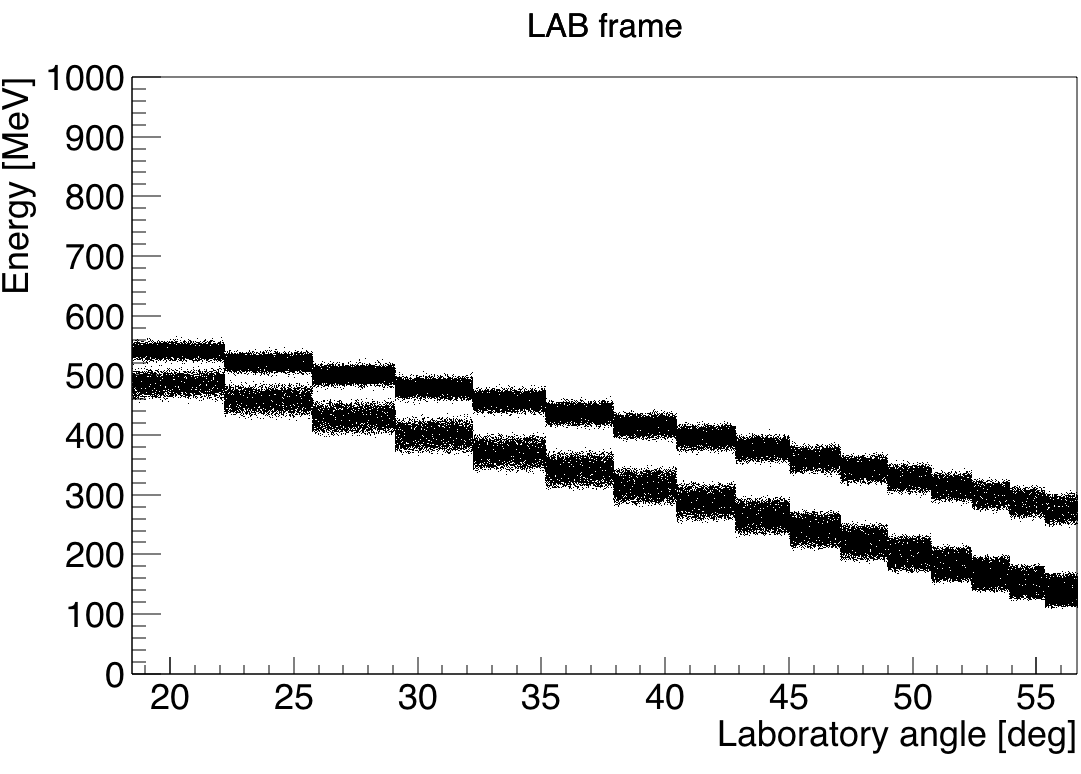
\includegraphics[width=\linewidth]{../Plots/simulation/kin_140Sm_208Pb.png}
	\caption{Simulation of the kinematics in the LAB frame for \Sm\ on \Pb\ at 4.65 MeV/u. The upper curve is the Sm and the lower curve is the Pb. Smaller angles corresponds to the inner rings and larger angles to the outer rings.}
	\label{fig:kinsim}
\end{figure}



\subsection{Online calibration of the particle detector}
Every year there is a campaign at ISOLDE, where the staff configures a settingsfile\footnote{For IS558, the settingsfile \textit{MBSettings2017\_CLX\_IS558.dat} was used.} if there are any changes in the setup system. In addition they run a coctail beam composed of different isotopes on a specific target to make a calibration file containing the calibration coefficients for the CD. For the \ga-detectors they put \ga\ sources in the target position and from the data they get the calibration coefficients which is put in the calibration file. This calibration file is adjusted for each experiment following the campaign period. In this way it is easy to sort and analyze during the experiment, check if it is going well and to make preliminary Doppler-corrected \ga-spectra. 


\bigskip

\textcolor{red}{\textbf{Trenger en overgang til M2R.}}

\bigskip



Just as for the \texttt{MedToRoot} program, a bash script named \texttt{Q4S.sh} was made for the \texttt{TreeBuilder} and \texttt{AQ4Sort} programs. 
\texttt{Q4S.sh} uses either \texttt{AQ4Sort} to make histograms for each pixel of the particle detector (used for calibration) or \texttt{Treebuilder} to build events, with a lot of files in one go for both. 
When using the online calibration, we don't need to use the \texttt{AQ4Sort} program, because we already have the calibration coefficients. 
They are adjusted in the beginning and during the experiment.
\texttt{TreeBuilder} makes event trees and energy spectra for both particle and \ga\ detection which can be used for analyzing the Coulomb excitation events.
The \textit{OnBeam.root}-files are loaded into \texttt{TreeBuilder} via \texttt{Q4S.sh} with the commands

\begin{lstlisting}[language=sh]
$ cd ~/GitHub/MasterThesis/Scripts/sorting 
$ ./Q4S.sh Sm online TB
... <showing output from script>
$ mv Sm_online-TreeBuilder-2019-06-24.root ../../Sorted_data/
\end{lstlisting}

Also other helping scripts to get histograms, do fitting, comparison and calibration was made. 
After the sorting, the file was moved to a folder of sorted data (with the \textbf{mv} command), and the relative path was given in the \textit{setup\_Sm.txt} file in \textit{Scripts/plotting/} used as input in the \texttt{ParticlePlot.cpp} script. 
This script has to be loaded into the ROOT 6 framework to extract the histograms of interest and fix the formatting.
To run the \texttt{ParticlePlot.cpp} in interaction with ROOT, the following commands are used

\begin{lstlisting}[language=sh]
$ cd ~/GitHub/MasterThesis/Scripts/plotting 
$ root
root [0] .L ParticlePlot.cpp++
root [1] plot_front_back_energy("setup_Sm.txt", "online")
... <showing output from script>
\end{lstlisting}

\autoref{fig:cal_online} shows the back vs. front energy (online calibration) for the four different quadrants of the CD. 
The plots shows a part of a line for each front and back strip. An indication of a good calibration is when all detectors lie on a linear line ($y = x$), meaning that the front side and the back side of the CD has detected the same energy. 
From the figure we see that not all detectors fit the line, indicating that there are some calibration coefficients wrong in some of the strips.
One major problem with the online calibration is that a number of the back strips have the wrong gains as shown in \autoref{fig:cal_CD_back}.





\subsection{User calibration of the particle detector}
An ambitious goal of the calibration was to make a program that could automatically fit the centroid of the peaks needed. 
It turned out to be very difficult, and it became more and more manual labor. 
Because of the complex peak shapes, it is very hard to do an automatic fitting it seems. 
The peaks demands very much individual care, which is very difficult to do with a automatic program. 
In logarithmic scale (log-scale) the data looked more Gaussian distributed, but it is not the case in linear scale. 
For the centroids, it was very hard to tell in log-scale how precise the automatic fitting was. 

The total amount of annular strips to calibrate on the front side of the CD is 64 (4 quadrants $\cdot$ 16 rings). 
On the back side we have 48 secular strips (4 quadrants $\cdot$ 12 strips). 
To fully calibrate the CD, we need all the centroids of the peaks from both sides, 128 centroids (64 annular strips $\cdot$ 2 peaks/ring) on the front side and 1536 centroids (48 secular strips $\cdot$ 2 peaks/ring $\cdot$ 16 rings) on the back side. 
The total centroids to collect are 1664 centroids, and this is not a task one would want to do manually.
For a quick calibration, or a bare minimum calibration, one needs two peaks in each annular strip and two peaks in each secular strip, making it 224 centroids.
Taking more centroids than this makes it more precise. 
By taking more centroids, which is generally a good idea, it is possible to check for non-linearities or instabilities in time.


\autoref{fig:cal_FC} shows a flowchart of the programs, scripts and files used in the user calibration. 
The idea was to use the \textbf{kinsim3()} function from \texttt{kinsim3.cc} to simulate the data and the \texttt{Q4S.sh} script to sort the experimental data with \texttt{AQ4Sort} to get each pixel of the CD. 
This data could either be analyzed in ROOT with the \textbf{TBrowser()} or through different functions in \texttt{ParticlePlot.cpp}. 
From either ROOT or \texttt{ParticlePlot.cpp}, information about the range of the peaks and guesses of the centroids of Pb and Sm would be written down in input files used in \texttt{ParticleFit.cpp}. 
Here the automatic fitting would have used the input files to fit the peaks, collect the centroids and written them to output files which would have been used as input files in \texttt{particle-calibration.py}. 
In this Python script, the centroids would have been plotted and a linear regression method using least squares of a first degree polynomial fit\footnote{Polynomial fit: \url{https://docs.scipy.org/doc/numpy/reference/generated/numpy.polyfit.html}} would have fitted a line to re-produce the points. 
It would also write the gains and offsets to separate output files, which would be used as input in \texttt{ADC\_generator.py}. 
This Python script will write the calibration coefficients to the terminal, and from there it is possible to copy and paste it into the calibration file \textit{IS5558-user.cal}. 
This calibration file is then used to sort the data once more with \texttt{Q4S.sh} using \texttt{TreeBuilder} and the new calibration coefficients.
To visualize plots after a new calibration, either ROOT or \texttt{ParticlePlot.cpp} can be used. 
The gray boxes related to the \ga-calibration will be discussed in \autoref{sec:gamma}.

The downfall of the automatic "centroid collector" came when trying it on the secular strips of the CD. 
There is just too much individual differences to calibrate the secular strips with a simple script given a channel range for all 12 back strips. 
This was discovered way too late. 
There isn't any range to "rule them all", at least since the fitting function can behave very strange given a too small or too big range.
To implement a proper automatic fitting program, one would have to find a function with a negatively (left) skewed distribution or negative skewness (right modal), where most of the data is more than the mean. 
Sadly this was discovered too late to implement it. 

In some spectra it was very hard to determine the centroid of the Pb peaks. 
We tried to use additional data from experiment IS553 ($^{144}$Ba on $^{58}$Ni), which was right before our experiment. 
The reason for this was to try to get calibration for the lower energy spectra. 
But unfortunately the data from the IS553 experiment was a bad fit with our experiment. 
The fitting just didn't seem reliable.
It gave a steeper slope than the online calibration, which was very good to begin with. 
Looking at the front vs. back energy plots, the diagonal lines were almost disappearing in the middle, and they were a lot broader than the online calibration. 
One big problem of not using the Ni-data, was that we could not get any calibration coefficients for front ring 16 and maybe also 15 for Pb since the back strips had very few counts, even with a lot of data put into one \textit{.root}-file. 
But this problem we also found in the Ni-data.
It would have been nice with some low-energy points to calibrate as well as high-energy points. 
The calibration did appear to get worse in a few aspects. 
Firstly, the diagonal line in the front vs. back energy spectra was not as defined as the online calibration, but also the off-diagonal events seemed to increase, implying that there was an increase in the mismatch of front and back events. 
The latter could be due to the visualization coming from the z-scale, since we have a different number of events. 

Looking at the energy vs. channel plots, it was clear that something was not good.
We could clearly see that a Gaussian fit didn't work. 
Since the Gaussian distribution was a bad fit for the experimental data, a built in function in ROOT of a 4th degree polynomial was tried out to fit the complex peak shapes. The function sets the initial values of the parameters automatically for the predefined function.
\begin{equation}
	f(x) = p_0 + p_1 \cdot x + p_2 \cdot x^2 + p_3 \cdot x^3 + p_4 \cdot x^4
\end{equation}
It turned out that this didn't match the shapes either. 
Unfortunately there is no way of knowing if a data set is useful or not until you try it. 
It may be that the energy loss or target thickness was wrong, or that the beam energy was different, or that the simulation didn't account for all the details of the stopping. 
The only way to get a good calibration is to have as much data as possible and then kick out the bad data until there is a good fit. 
What was clear at the moment was that the scatter between the data points from different the reactions was too large to simply average out with a straight line fit. 
We have to select data that agree.

In the Sm data, the issue came in determining the peak centroid or maximum for the experimental data. 
The peak shape is a convolution of many effects; intrinsic resolution of the detector, the beam energy width, straggling in the target, interaction points in the target, angular width of the detector strip, etc. 
While the simulation tries to include all these things, we found that the peak shapes were not exactly the same. 
It might be worthwhile spending a bit of time to play with the parameters and try to get the peak shape as similar as possible. 
At that point, maybe use a certain feature of the peak, such as the maximum, or the highest energy edge. 
Or, honestly, it might be better to simply hover the mouse over the correct "feature" of the peak and position it by eye, be it the centroid or the maximum.
Then we can analyze the same feature in the corresponding simulated spectrum.
The maximum of the peak on the high energy side is not the center of the peak, but roughly equivalent to the maximum. 
You can imagine that fitting a Gaussian to the right-hand side (high-energy side) only, this would be roughly where the centroid is. 

The innermost ring of the CD was very damaged by the bombardment of particles hitting it, so we had to remove the innermost ring from the data set (making the total centroids to collect to be 1500). 
In the innermost ring, it was impossible to separate the beam and target peaks.
This is unfortunate since the innermost ring has the most statistics, but Si detectors don't last forever. 
It was old and supposed to be changed after our experiment. 
We also found something weird with quadrant 4 secular strip 1 (Q4\_b1), it shows a lot more counts than all the other back strips. 
Excluding detector strips is easy, the only thing to do is to set gain and offset to -1 (or gain to 0 and offset to -1). 
That will make the energy calibration negative, and fall out of the scope. 
It is the way it is usually done for dead CD strips or dead \ga-detectors. 

\bigskip

\textcolor{red}{\textbf{Trenger en overgang her..}}

\bigskip

Changing the relative path in the \textit{setup\_Sm.txt} file used as input in the \texttt{ParticlePlot.cpp} script, we now have


\begin{lstlisting}[language=sh]
$ cd ~/GitHub/MasterThesis/Scripts/sorting 
$ ./Q4S.sh Sm user TB
... <showing output from script>
$ mv Sm_user-TreeBuilder-2019-06-20.root ../../Sorted_data/
\end{lstlisting}



\subsubsection*{TreeBuilder}
\begin{lstlisting}[language=]
$ ./Q4S.sh Sm user TB
--- TreeBuilder ---
input file(s):
... <shows a list of all input files>
output file: Sm_user-TreeBuilder-2019-06-20.root
calibration file: ../../Miniball-config/IS558-user.cal
WeightPR: 0.75
Particle distribution:
 Q0 fired: 12243817
 Q1 fired: 12277727
 Q2 fired: 11479362
 Q3 fired: 10936096
Finished.
\end{lstlisting}


\subsubsection*{AQ4Sort}
\begin{lstlisting}[language=]
$ ./Q4S.sh Sm user Q4
Info: No flag option for 'AQ4Sort'. Ignoring optional flag.
--- AQ4Sort ---
calibration file: ../../Miniball-config/IS558-user.cal
input file(s):
... <shows a list of all input files>
output file: Sm_user-AQ4Sort-2019-06-24.root
\end{lstlisting}


\autoref{fig:cal_ED} shows one strip that is easy to calibrate and one that is difficult to calibrate.

\begin{figure}[ht]
	\centering
	\begin{subfigure}{\textwidth}
		\centering
		% get_single_plot("setup_Sm.txt", "tb", "f", 0, 4, 9, 1, 300, 2400, 1080)
		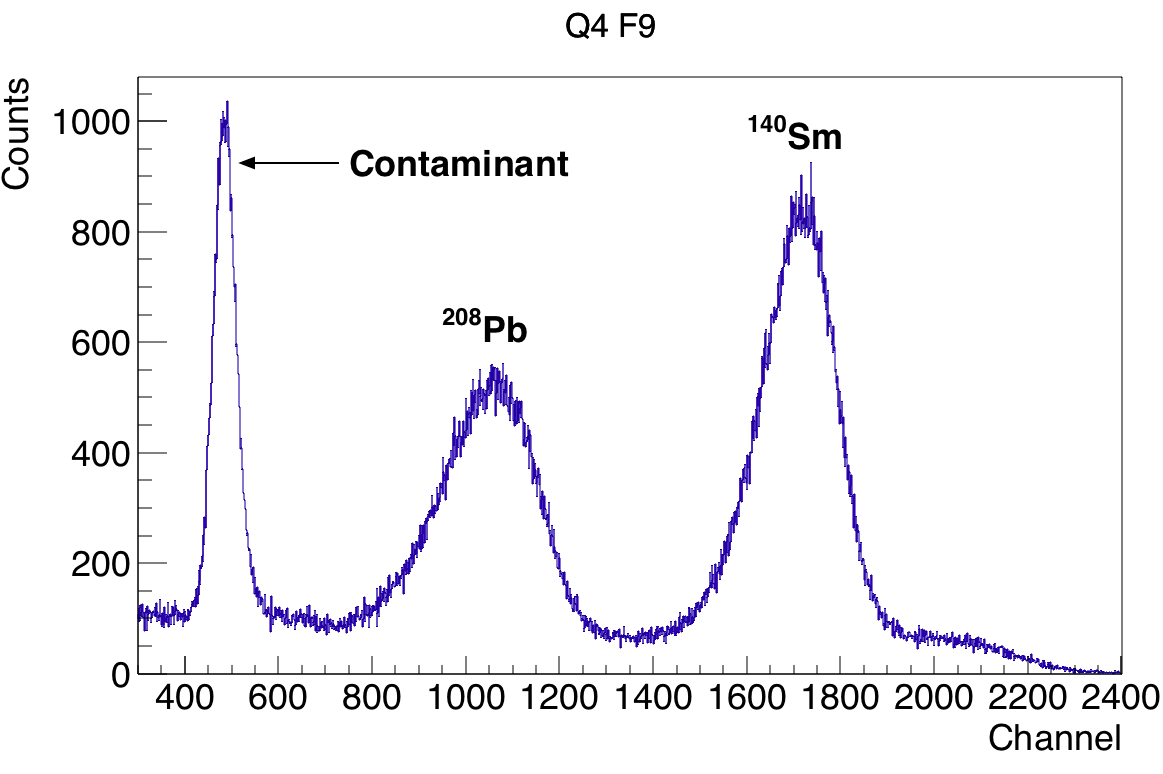
\includegraphics[width=\textwidth]{../Plots/plotting/TB_Q4_F9.png}
		\caption{Easy.}
		\label{fig:cal_easy}
	\end{subfigure}
	\begin{subfigure}{\textwidth}
		\centering
		% get_single_plot("setup_Sm.txt", "q4", "b", 0, 1, 16, 12, 200, 1400, 330)
		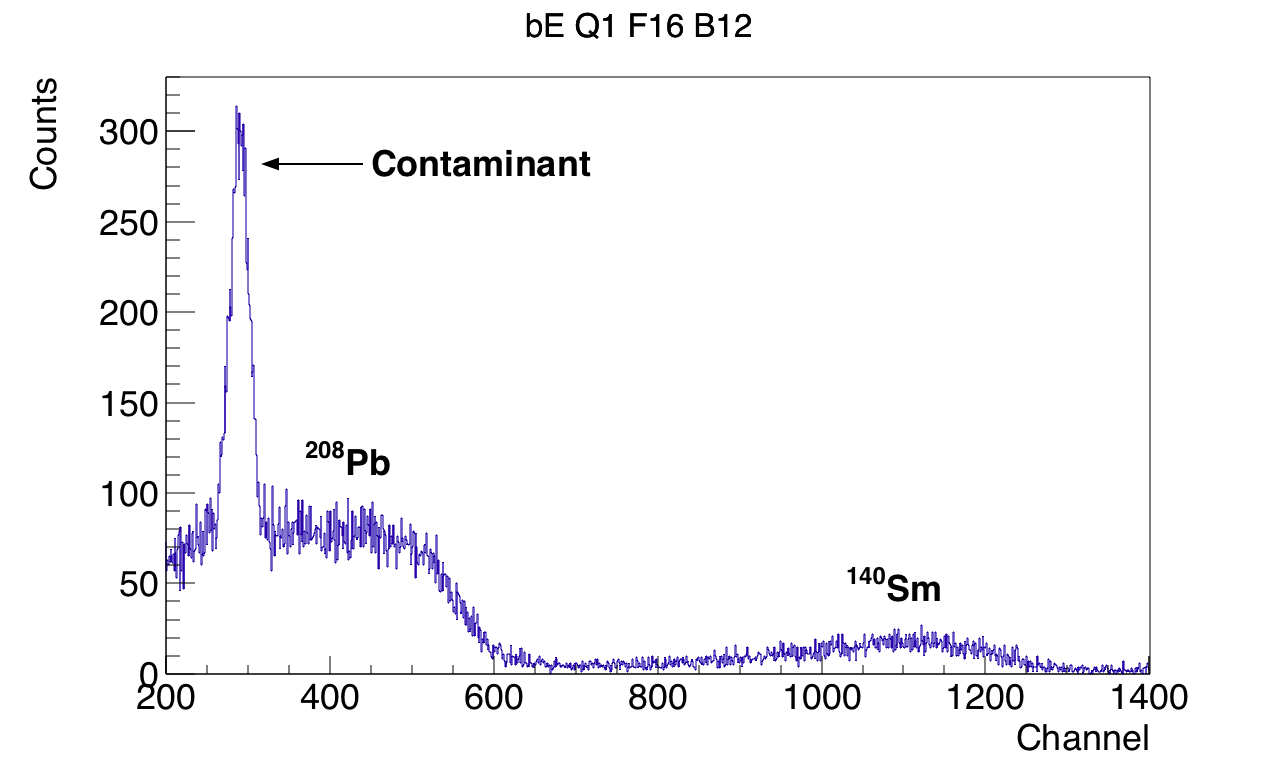
\includegraphics[width=\textwidth]{../Plots/plotting/bE_Q1_f16_b12.png}
		\caption{Difficult.}
		\label{fig:cal_difficult}
	\end{subfigure}
	\caption{Cal.}
	\label{fig:cal_ED}
\end{figure}


The user calibration of the CD shown in \autoref{fig:cal_user} is basically the online calibration without the innermost ring. 


\begin{figure}[ht]
	\centering
	\begin{subfigure}{\textwidth}
		\centering
		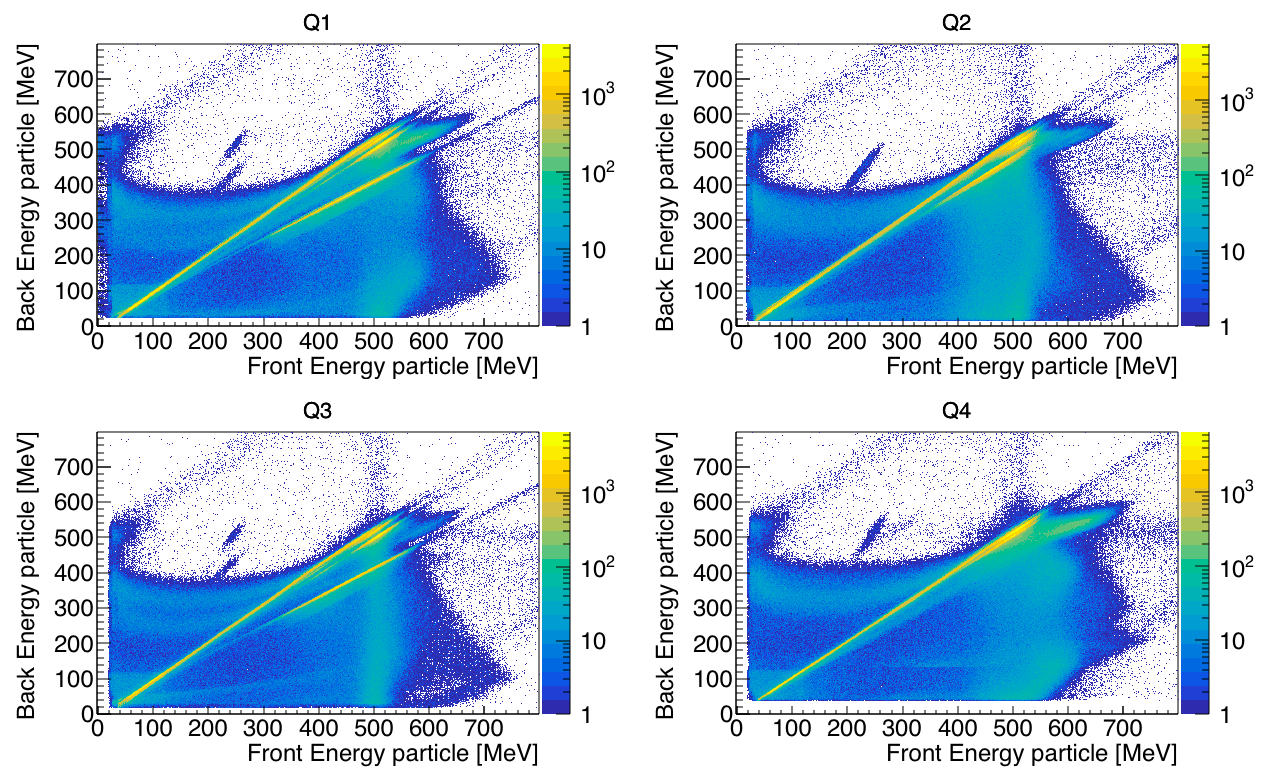
\includegraphics[width=\textwidth]{../Plots/plotting/E_f_b_Q1-4-online.png}
		\caption{Online calibration for the CD showing the four quadrants. It generally looks quite good, but there is a number of the secular strips (back side) that have the wrong gains.}
		\label{fig:cal_online}
	\end{subfigure}
	\begin{subfigure}{\textwidth}
		\centering
		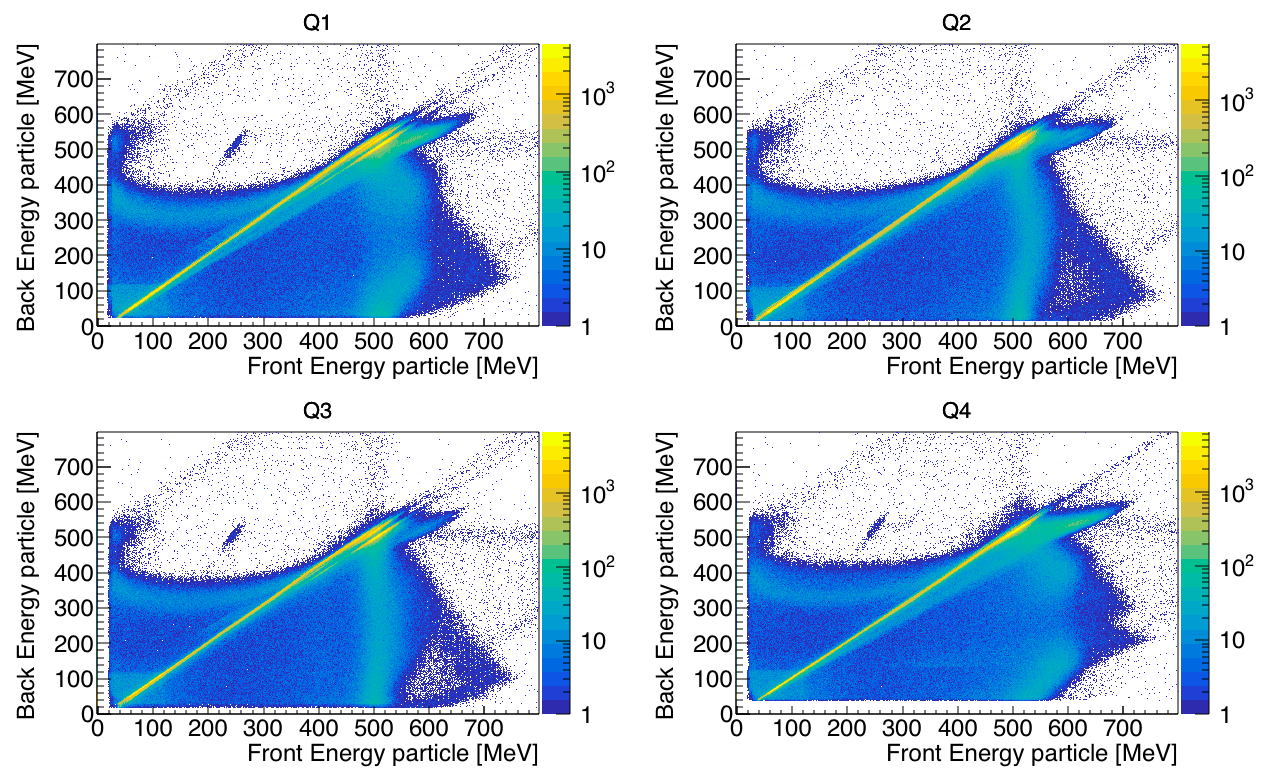
\includegraphics[width=\textwidth]{../Plots/plotting/E_f_b_Q1-4-user.png}
		\caption{User calibration for the CD showing the four quadrants. This is actually the online calibration without the innermost ring which was broken.}
		\label{fig:cal_user}
	\end{subfigure}
	\caption{Back energy vs. front energy for each quadrant of the CD.}
	\label{fig:cal_OU}
\end{figure}


% CD energy vs. strip -->
%
%\begin{lstlisting}[language=sh]
%$ cd /Users/trondwj/GitHub/MasterThesis/Scripts/plotting 
%$ root
%root [0] .L ParticlePlot.cpp++
%root [1] CD_energy("setup_Sm.txt", "f")
%\end{lstlisting}
%
%\begin{lstlisting}[language=sh]
%$ cd /Users/trondwj/GitHub/MasterThesis/Scripts/plotting 
%$ root
%root [0] .L ParticlePlot.cpp++
%root [1] CD_energy("setup_Sm.txt", "b")
%\end{lstlisting}
%
% CD energy vs. strip --<

\begin{figure}[ht]
	\centering
	\begin{subfigure}{\textwidth}
		\centering
		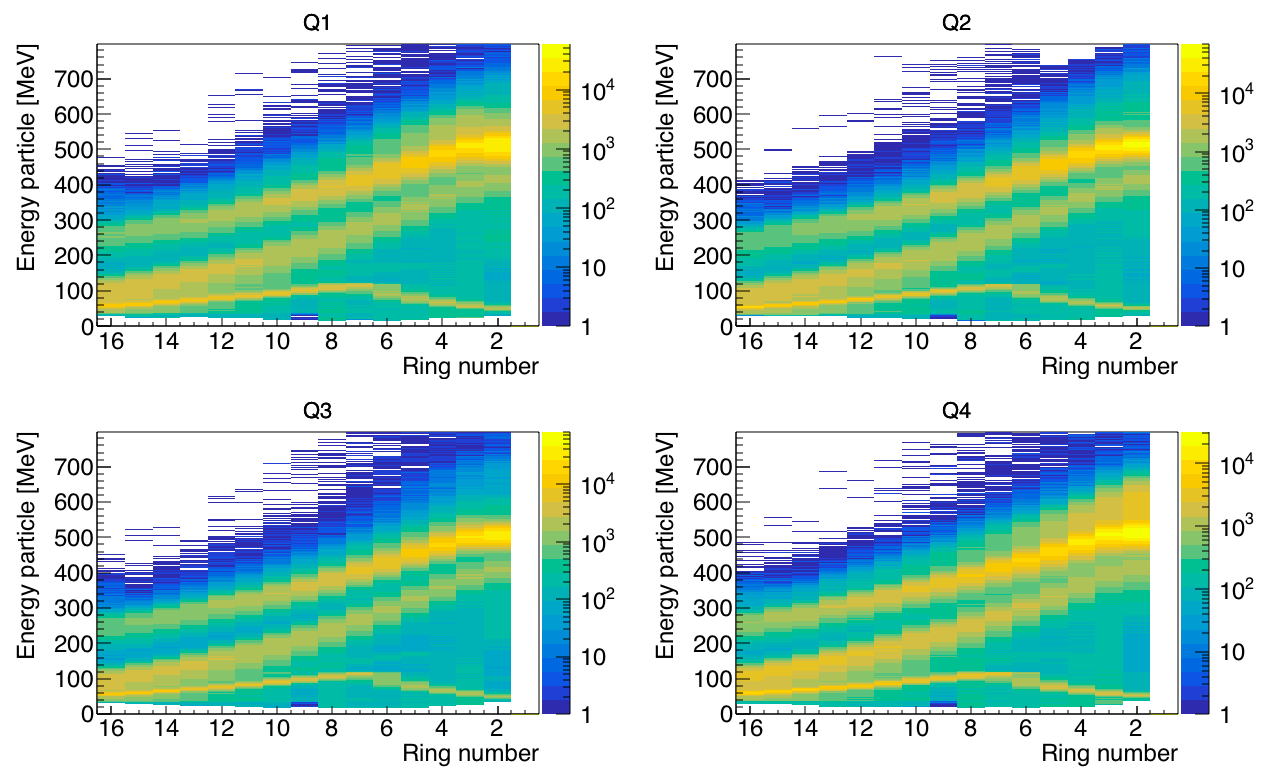
\includegraphics[width=\textwidth]{../Plots/plotting/E_vs_f-strip_all_Q.png}
		\caption{CD front. Ring number 16 is the outermost ring and ring number 1 is the innermost ring.}
		\label{fig:cal_CD_front}
	\end{subfigure}
	\begin{subfigure}{\textwidth}
		\centering
		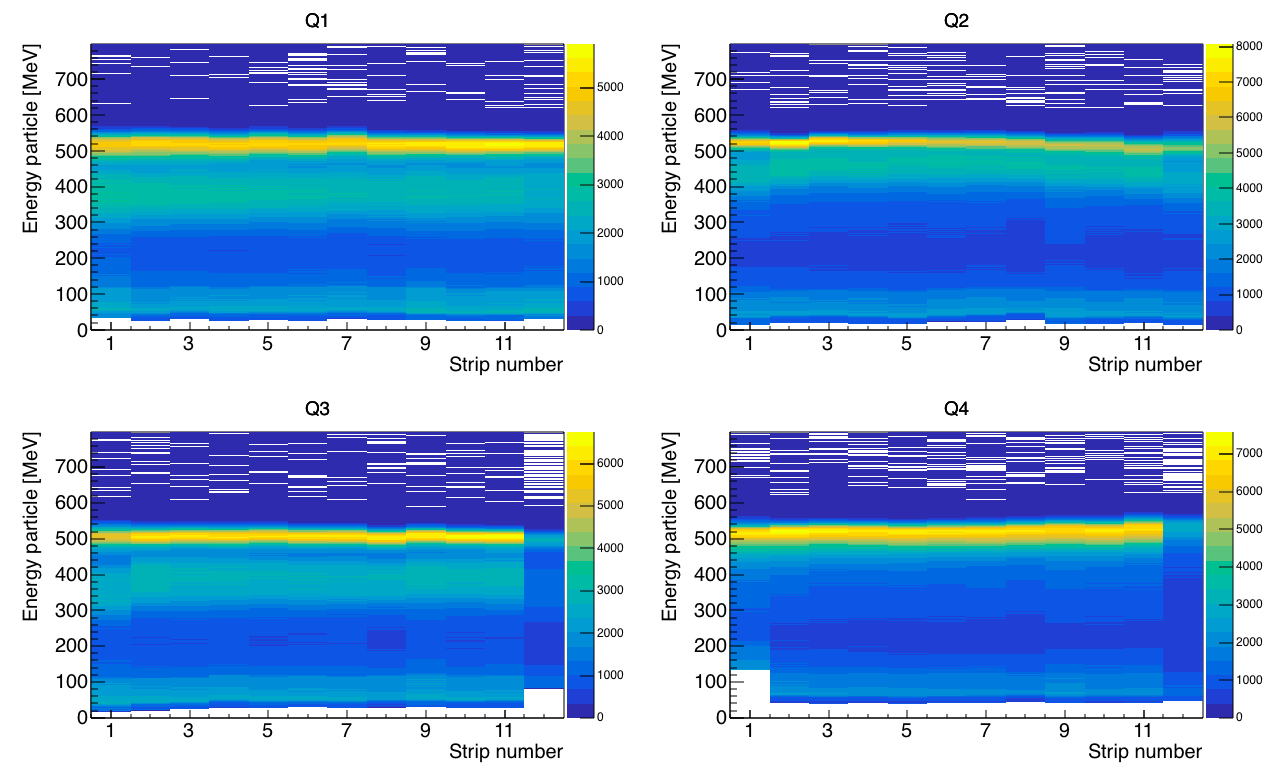
\includegraphics[width=\textwidth]{../Plots/plotting/E_vs_b-strip_all_Q.png}
		\caption{CD back. A number of the secular strips have the wrong gains.}
		\label{fig:cal_CD_back}
	\end{subfigure}
	\caption{Energy vs. strip number for each quadrant of the CD.}
	\label{fig:cal_CD}
\end{figure}



\begin{figure}[ht]
	\centering
	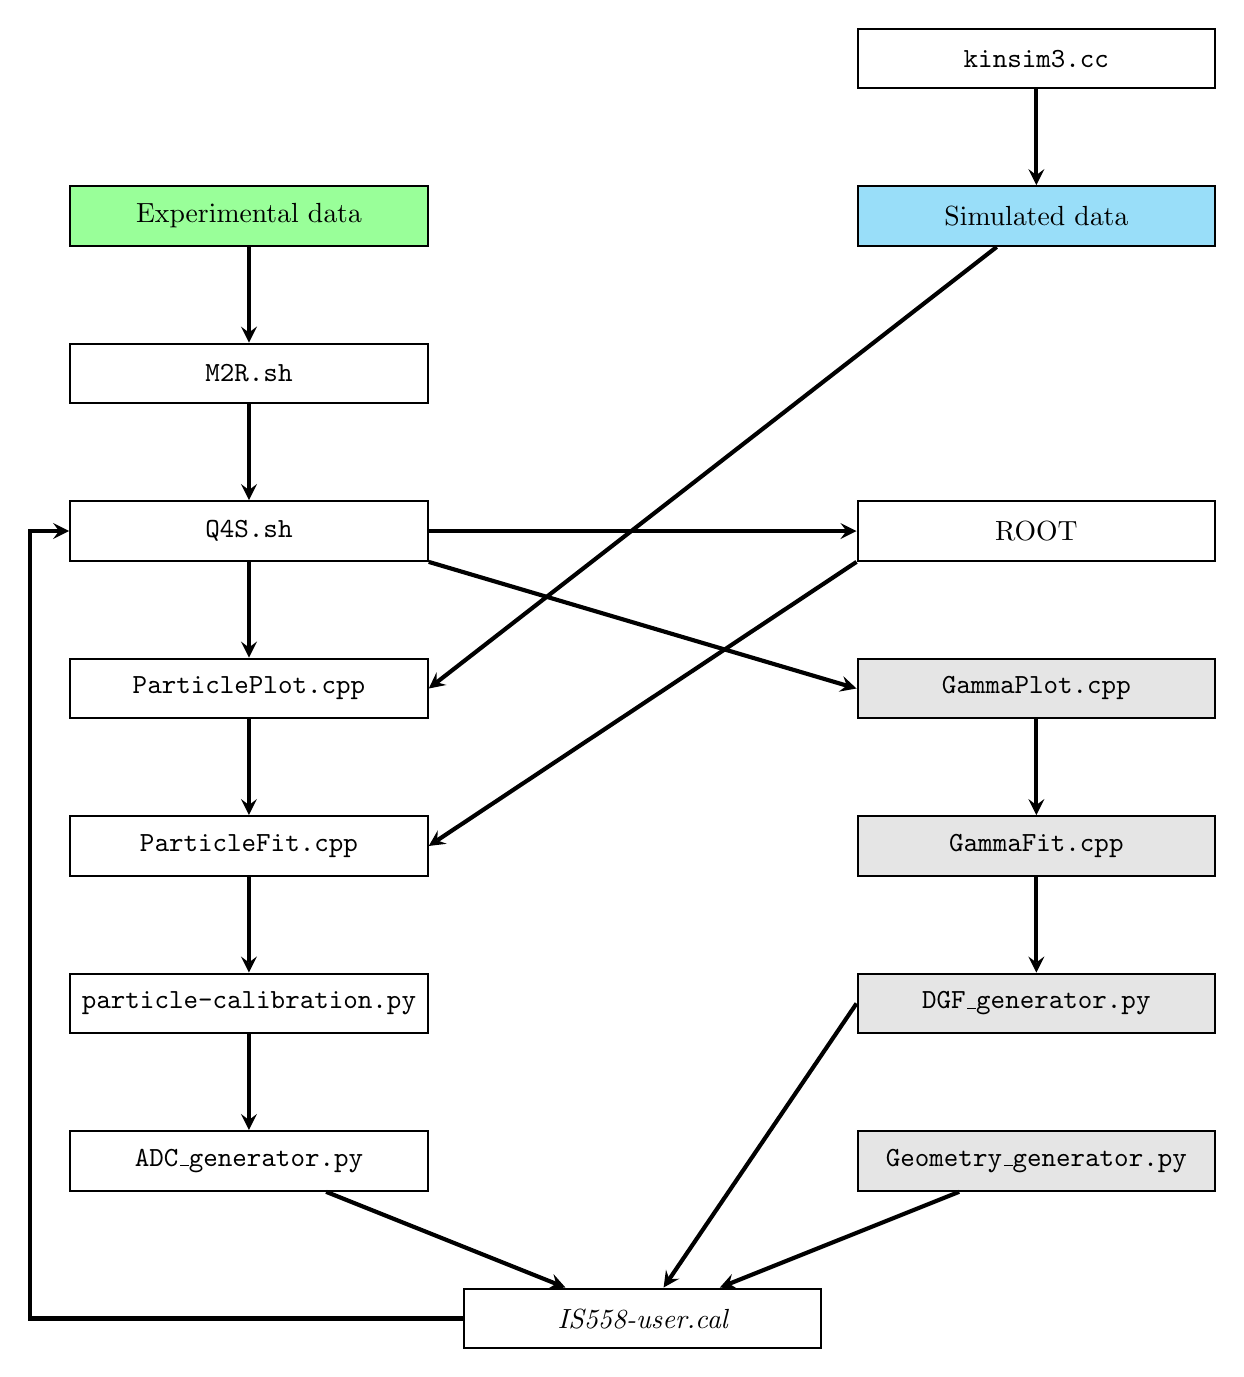
\begin{tikzpicture}[
    box/.style = { draw,minimum width=+30ex,minimum height=+5ex,thick },
    arrowstyle/.style = { ->,>=stealth,line width=1.5pt }
    ]
    % Definitions
    \coordinate (ks3)  at ( 5, 2 );
    \coordinate (sim)  at ( 5, 0 );
    \coordinate (exp)  at (-5, 0 );
    \coordinate (M2R)  at (-5,-2 );
    \coordinate (Q4S)  at (-5,-4 );
    \coordinate (Pplt) at (-5,-6 );
    \coordinate (Pfit) at (-5,-8 );
    \coordinate (pcal) at (-5,-10);
    \coordinate (Pgen) at (-5,-12);
    \coordinate (ROOT) at ( 5,-4 );
    \coordinate (Gplt) at ( 5,-6 );
    \coordinate (Gfit) at ( 5,-8 );
    \coordinate (Dgen) at ( 5,-10);
    \coordinate (Ggen) at ( 5,-12);
    \coordinate (calf) at ( 0,-14);
    % Nodes
    \node(K)  at (ks3)  [box]               {$\texttt{kinsim3.cc}$};
    \node(S)  at (sim)  [box,fill=cyan!40]  {Simulated data};
    \node(E)  at (exp)  [box,fill=green!40] {Experimental data};
    \node(M)  at (M2R)  [box]               {$\texttt{M2R.sh}$};
    \node(A)  at (Q4S)  [box]               {$\texttt{Q4S.sh}$};
    \node(RT) at (ROOT) [box]               {ROOT};
    \node(PP) at (Pplt) [box]               {$\texttt{ParticlePlot.cpp}$};
    \node(PF) at (Pfit) [box]               {$\texttt{ParticleFit.cpp}$};
    \node(pc) at (pcal) [box]               {$\texttt{particle-calibration.py}$};
    \node(ag) at (Pgen) [box]               {$\texttt{ADC\_generator.py}$};
    \node(GP) at (Gplt) [box,fill=black!10] {$\texttt{GammaPlot.cpp}$};
    \node(GF) at (Gfit) [box,fill=black!10] {$\texttt{GammaFit.cpp}$};
    \node(dg) at (Dgen) [box,fill=black!10] {$\texttt{DGF\_generator.py}$};
    \node(gg) at (Ggen) [box,fill=black!10] {$\texttt{Geometry\_generator.py}$};
    \node(cf) at (calf) [box]               {$\textit{IS558-user.cal}$};
    % Arrows
    \draw[arrowstyle] (K)             -- (S);
    \draw[arrowstyle] (E)             -- (M);
    \draw[arrowstyle] (M)             -- (A);
    \draw[arrowstyle] (S)             -- (PP.east);
    \draw[arrowstyle] (A)             -- (PP);
    \draw[arrowstyle] (A.east)        -- (RT.west);
    \draw[arrowstyle] (A.south east)  -- (GP.west);
    \draw[arrowstyle] (RT.south west) -- (PF.east);
    \draw[arrowstyle] (PP)            -- (PF);
    \draw[arrowstyle] (PF)            -- (pc);
    \draw[arrowstyle] (pc)            -- (ag);
    \draw[arrowstyle] (ag)            -- (cf);
    \draw[arrowstyle] (GP)            -- (GF);
    \draw[arrowstyle] (GF)            -- (dg);
    \draw[arrowstyle] (dg.west)       -- (cf);
    \draw[arrowstyle] (gg)            -- (cf);
    \draw[arrowstyle] (cf.west)       |- node[] {} ++(-5.5,0) |- (A.west);
\end{tikzpicture}
	\caption{Flowchart of the programs, scripts and files used in the user calibration. The relative paths of these programs and scripts is shown in \autoref{tab:paths}.}
	\label{fig:cal_FC}
\end{figure}



It was anyways decided to stick with the online calibration for this thesis since there is no time to do a new calibration of the detectors. 
A lot of time have been used on scripts, and then the auto-fitting was a much harder problem than first expected (because of the shape of the peaks). 

\bigskip

\textcolor{red}{Skal jeg forklare mer om "the fitting procedure" i denne seksjonen?}


\subsection{Threshold}
The continuum of events at low energy comes from charge sharing between the strips.
 \autoref{fig:Pedestal} shows the big peak of the charge sharing on the front and back side. 
 This peak we call the "pedestal", because it is like a massive statue in front of the interesting data. 
 For the very heavy ions, the total amount of charge deposited gets split between neighboring strips of the CD. 
There is a single common gate for each ADC, containing channels from one CD quadrant. 
Therefore, when there is an event in one strip of the CD all channels are readout, but the channels without a real event read a "zero" energy.
These are the events in the pedestal.
One should define the threshold for each ADC channel to be above this peak.
After a correct calibration is applied, this pedestal will be calibrated out of the physical energy range.

\textsl{MiniballCoulexSort} does perform some tricks to try to recover the correct energy and position, but that depends on counting the number of strips that fire. 
We use a software threshold to cut away the pedestal. 
If the threshold is set too low, we will include pedestal events and it will get things wrong. 
If the threshold is too high, we will miss some events that have charge sharing and get the wrong energy for the particle. 
The goal is to not include the pedestal, and don't cut away too many events from the continuum.
It is easier to set thresholds in linear scale than logarithmic, because in logarithmic scale the threshold value will decrease very much and it's hard to see where to set the limit. 
The default threshold (if none is given in the calibration file) is set to channel 100. 
In some cases this is too much and in others this is not enough. 
For each ADC channel, the threshold can, and should be set. 
\autoref{fig:Threshold} shows the software threshold set in the calibration file on the front and back side for one strip on each side.





\textcolor{Magenta}{Tilbakemelding: \newline 
I presume that charge sharing is only considered if 2 firing strips are neighbors?
}


% Pedestal -->
%
%\begin{lstlisting}[language=sh]
%$ cd /Users/trondwj/GitHub/MasterThesis/Scripts/plotting 
%$ root
%root [0] .L ParticlePlot.cpp++
%root [1] check_pedestal("setup_Sm.txt", "f", 2, 4, 60)
%\end{lstlisting}
%
%\begin{lstlisting}[language=sh]
%$ cd /Users/trondwj/GitHub/MasterThesis/Scripts/plotting 
%$ root
%root [0] .L ParticlePlot.cpp++
%root [1] check_pedestal("setup_Sm.txt", "b", 3, 8, 70)
%\end{lstlisting}
%
% Pedestal --<

\begin{figure}[ht]
	\centering
	\begin{subfigure}{\textwidth}
		\centering
		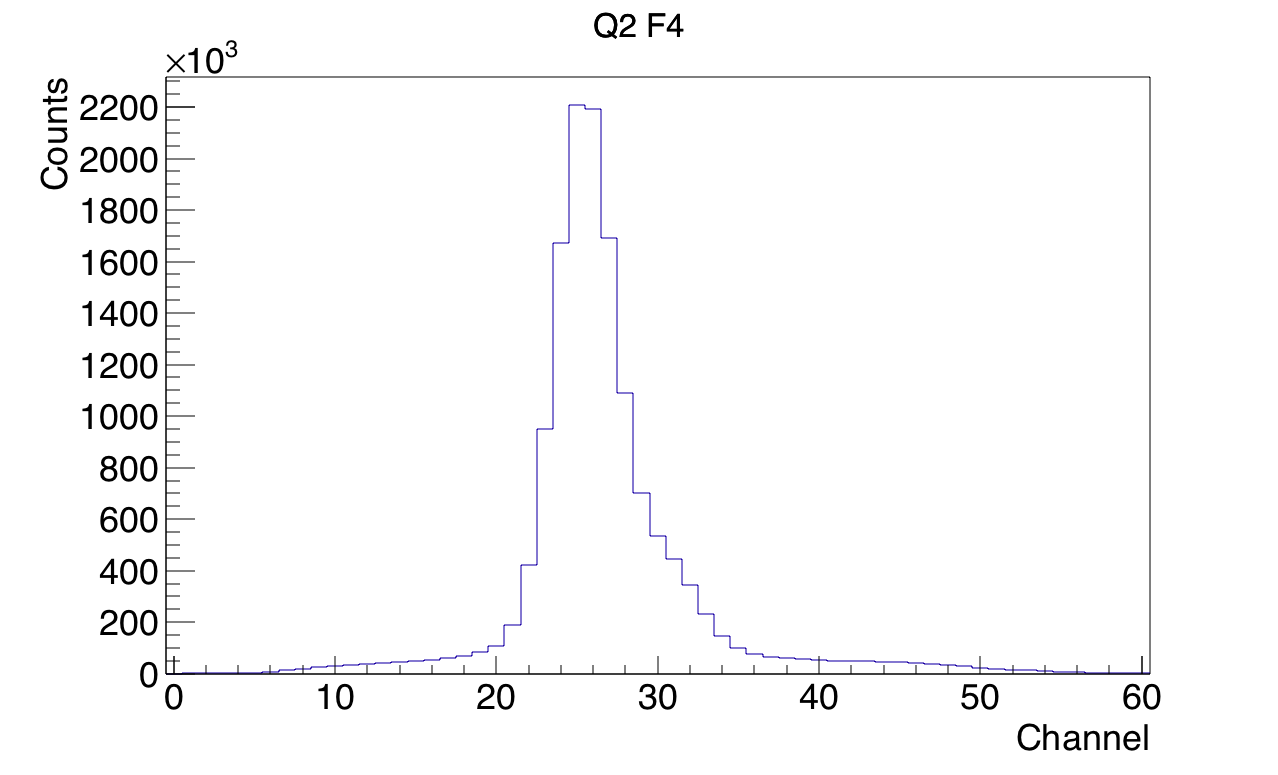
\includegraphics[width=\textwidth]{../Plots/plotting/Pedestal_Q2_f4.png}
		\caption{Pedestal in quadrant 2, annular strip 4.}
		\label{fig:Pedestal_f}
	\end{subfigure}
	\begin{subfigure}{\textwidth}
		\centering
		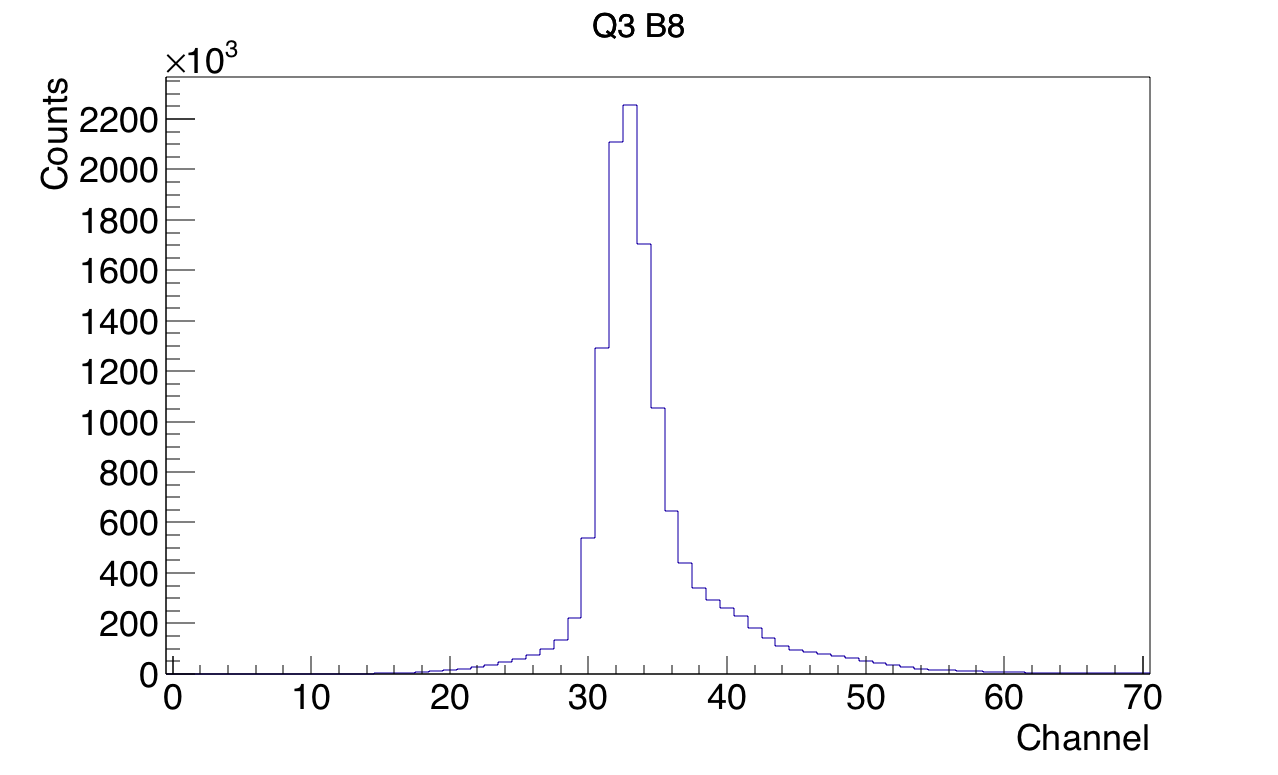
\includegraphics[width=\textwidth]{../Plots/plotting/Pedestal_Q3_b8.png}
		\caption{Pedestal in quadrant 3, secular strip 8.}
		\label{fig:Pedestal_b}
	\end{subfigure}
	\caption{The pedestal from charge sharing in the front and back side of the CD.}
	\label{fig:Pedestal}
\end{figure}


% Threshold -->
%
%\begin{lstlisting}[language=sh]
%$ cd /Users/trondwj/GitHub/MasterThesis/Scripts/plotting 
%$ root
%root [0] .L ParticlePlot.cpp++
%root [1] check_single_threshold("setup_Sm.txt", "f", 1, 11, 2100, 1500)
%\end{lstlisting}
%
%\begin{lstlisting}[language=sh]
%$ cd /Users/trondwj/GitHub/MasterThesis/Scripts/plotting 
%$ root
%root [0] .L ParticlePlot.cpp++
%root [1] check_single_threshold("setup_Sm.txt", "b", 1, 6, 2800, 1500)
%\end{lstlisting}
%
% Threshold --<

\begin{figure}[ht]
	\centering
	\begin{subfigure}{\textwidth}
		\centering
		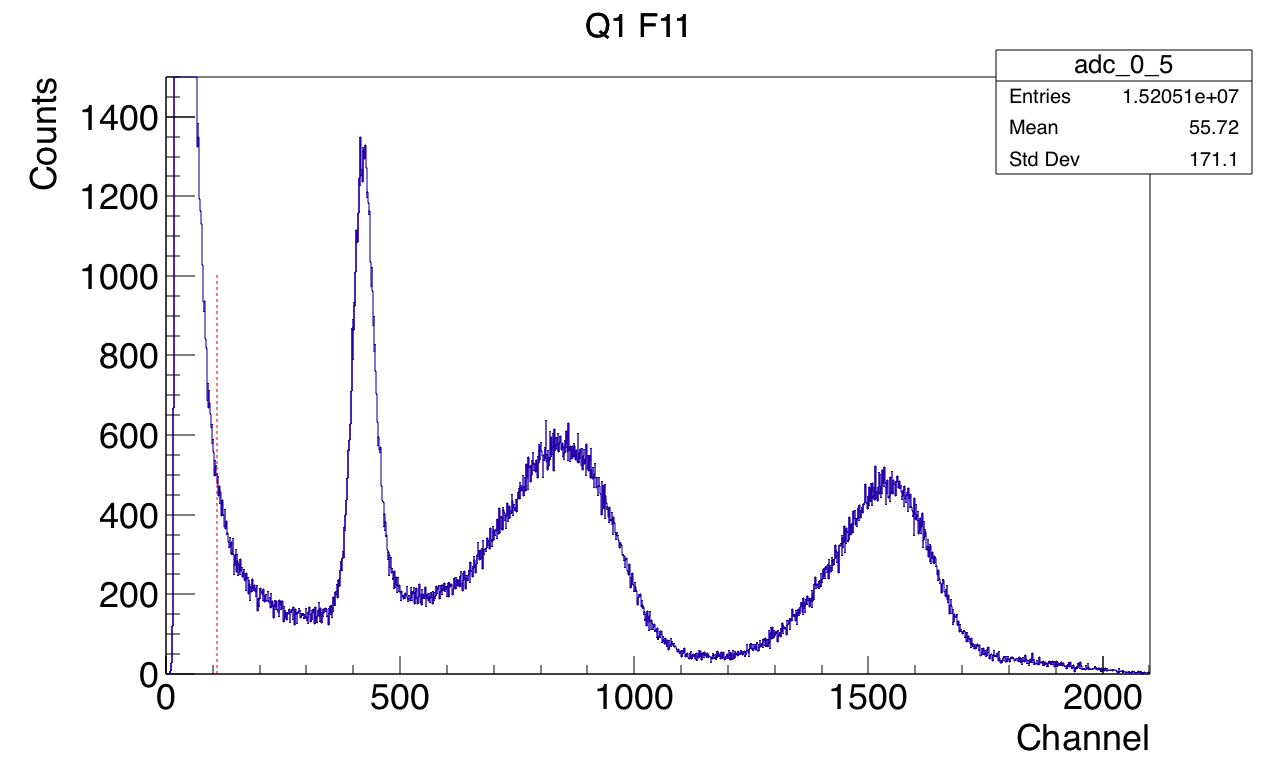
\includegraphics[width=\textwidth]{../Plots/plotting/Threshold_Q1_f11.png}
		\caption{Threshold Q1, F11.}
		\label{fig:Threshold_f}
	\end{subfigure}
	\begin{subfigure}{\textwidth}
		\centering
		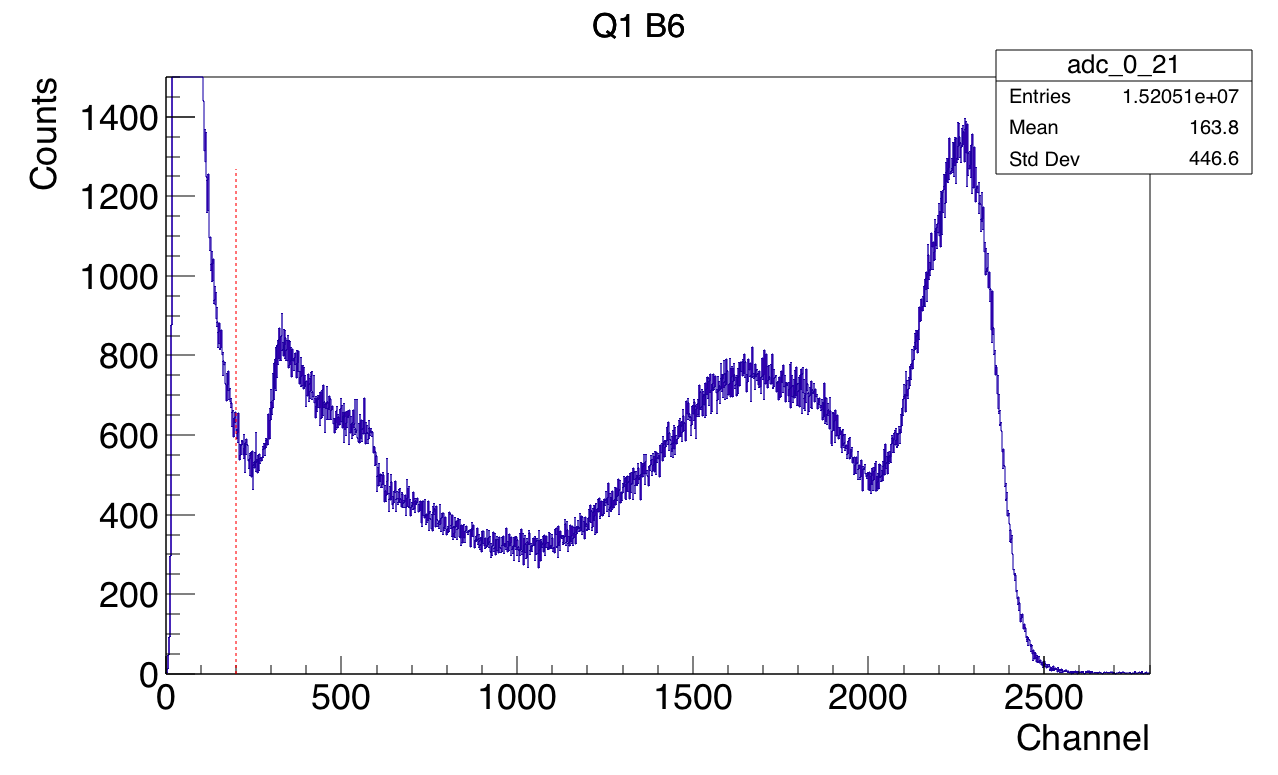
\includegraphics[width=\textwidth]{../Plots/plotting/Threshold_Q1_b6.png}
		\caption{Threshold Q1, B6.}
		\label{fig:Threshold_b}
	\end{subfigure}
	\caption{??}
	\label{fig:Threshold}
\end{figure}


The key spectra to look at are \autoref{fig:part} and \autoref{fig:CD_debug}. 
\autoref{fig:CD_debug} shows how many particles have strips fired on the front side or back side of the CD (counts how many particles have X strips fired on the front side and Y strips fired on the back side). 
The debug IDs are explained by \autoref{tab:CD_debug}. 
If we have too many debug ID = 3, then the threshold is too low. If we have a large continuum/background in \autoref{fig:part}, the thresholds are too high. The best thing to do is to play about with different values to see what is best.
Debug ID 20 is when no particle can be found, because there is no energy registered in either the front or the back strips. 
This can only happen when the front energy is below the software threshold set by the user in the calibration file and the back energy is either in a broken strip or is also below the software threshold. 
It is likely that it is some noise events or charge sharing that comes below the threshold. 



\begin{figure}[ht]
	\centering
	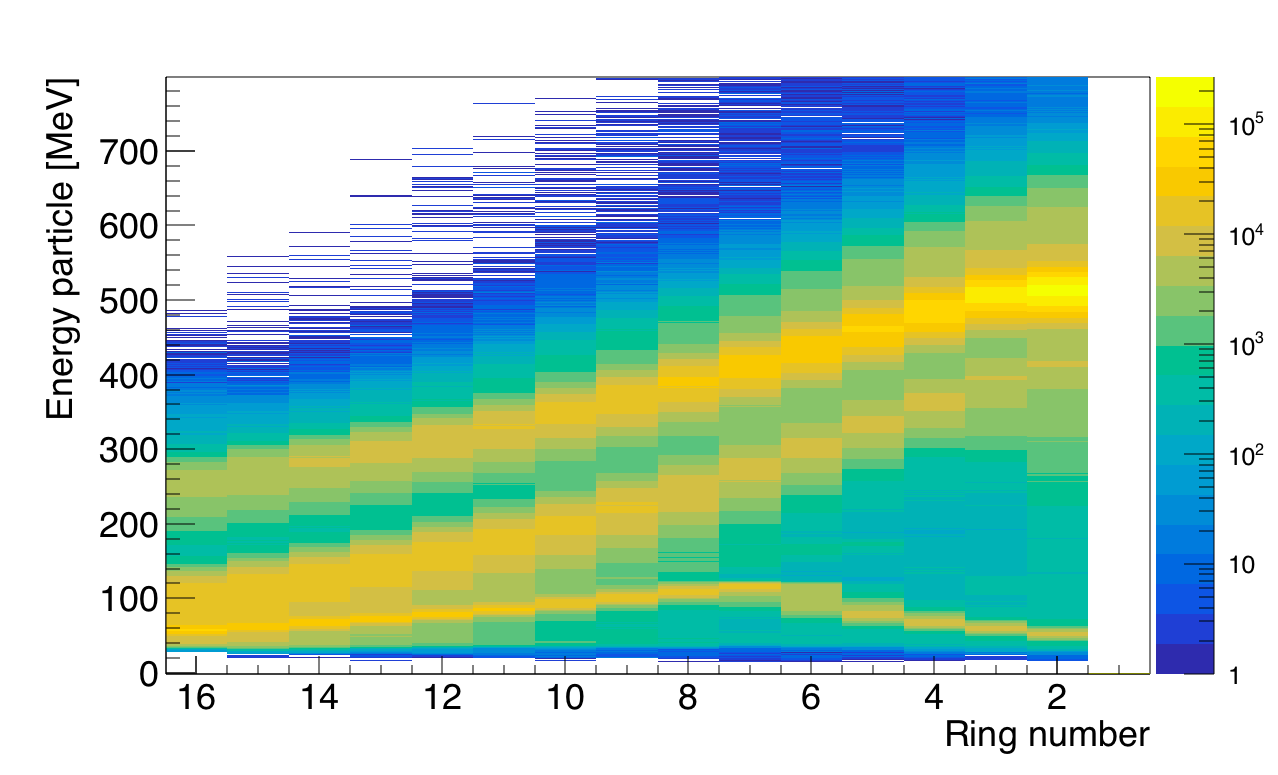
\includegraphics[width=\textwidth]{../Plots/plotting/E_vs_ring_all.png}
	\caption{Energy vs. ring number.}
	\label{fig:part}
\end{figure}


%\begin{lstlisting}[language=sh]
%$ cd /Users/trondwj/GitHub/MasterThesis/Scripts/plotting 
%$ root
%root [0] .L ParticlePlot.cpp++
%root [1] check_cd_debug("setup_Sm.txt", "user")
%\end{lstlisting}

\begin{figure}[ht]
	\centering
	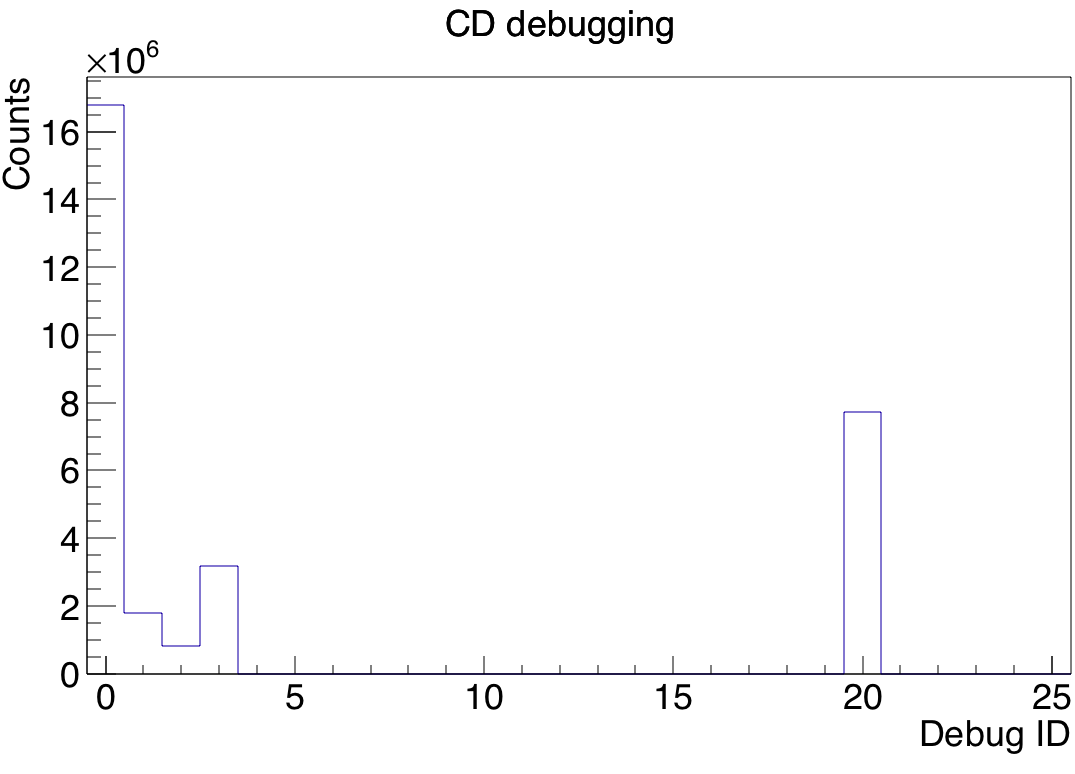
\includegraphics[width=\textwidth]{../Plots/plotting/cd_debug-user.png}
	\caption{CD debugging. Debug IDs are explained by \autoref{tab:CD_debug}. }
	\label{fig:CD_debug}
\end{figure}

\begin{table}[ht] 
	\centering 
	\caption{CD debugging.}
	% Data for the CD angles table
\begin{tabular}{ccc}
\hline
             &  \multicolumn{2}{c}{Strips fired}       \\
CD debug ID  &  Front side &  Back side                \\
\hline
0            &     1       &     1                     \\
1            &     1       &     2                     \\
2            &     2       &     1                     \\
3            &  $>$1       &  $>$1                     \\
20           &  \multicolumn{2}{c}{No particle found}  \\
\hline
\end{tabular}
	\label{tab:CD_debug}
\end{table}



\subsection{Time structure and calibration}
Each quadrant of the CD is independently connected to a Time to Digital Converter (TDC), which keeps track of the time of registered particle-\ga\ \textcolor{red}{(and particle-\ga-\ga)?} coincidences. 
The ADCs and DGFs record an energy and a time-stamp with 25 ns ticks. 
It is the multiplicity of the output of the DGFs that is used to generate the \ga\ signal, which in turn is used to make the particle-\ga\ coincidence.
\autoref{fig:ITS} shows a schematic of the ISOLDE time structure. 
The Miniball data acquisition is happening during two time windows, the "on-beam" and "off-beam" windows. 
When REXEBIS releases the beam to the HIE-ISOLDE LINAC, a signal is also sent to generate the on-beam window. 
This window called the "slow extraction mode" was 800 $\mu$s, but in 2011 it was extended to 1 ms, because the method of extraction of the beam was improved. 
All the data are read out after the on-beam window. 
This causes the DAQ to become dead for a while, so the next on-beam window is triggered when the DAQ is operable again.
The off-beam window starts 60 $\mu$s after the end of a readout, triggered by the disappearance of the DAQ is inoperable signal, to then allow the ADCs and TDCs time to start. 
In the off-beam window, which has the same duration of time as the on-beam window, data recordings of the background is conducted.
After the off-beam window closes, a readout of the records is triggered.
It is then possible to subtract the windows from each other to get the beam contribution. 
The DAQ system records the signals from each detector segment, which is individually time-stamped. 
With these records, a full reconstruction of the real events and coincidences is possible \cite{NWarr-el}.


\begin{figure}[ht]
	\centering
	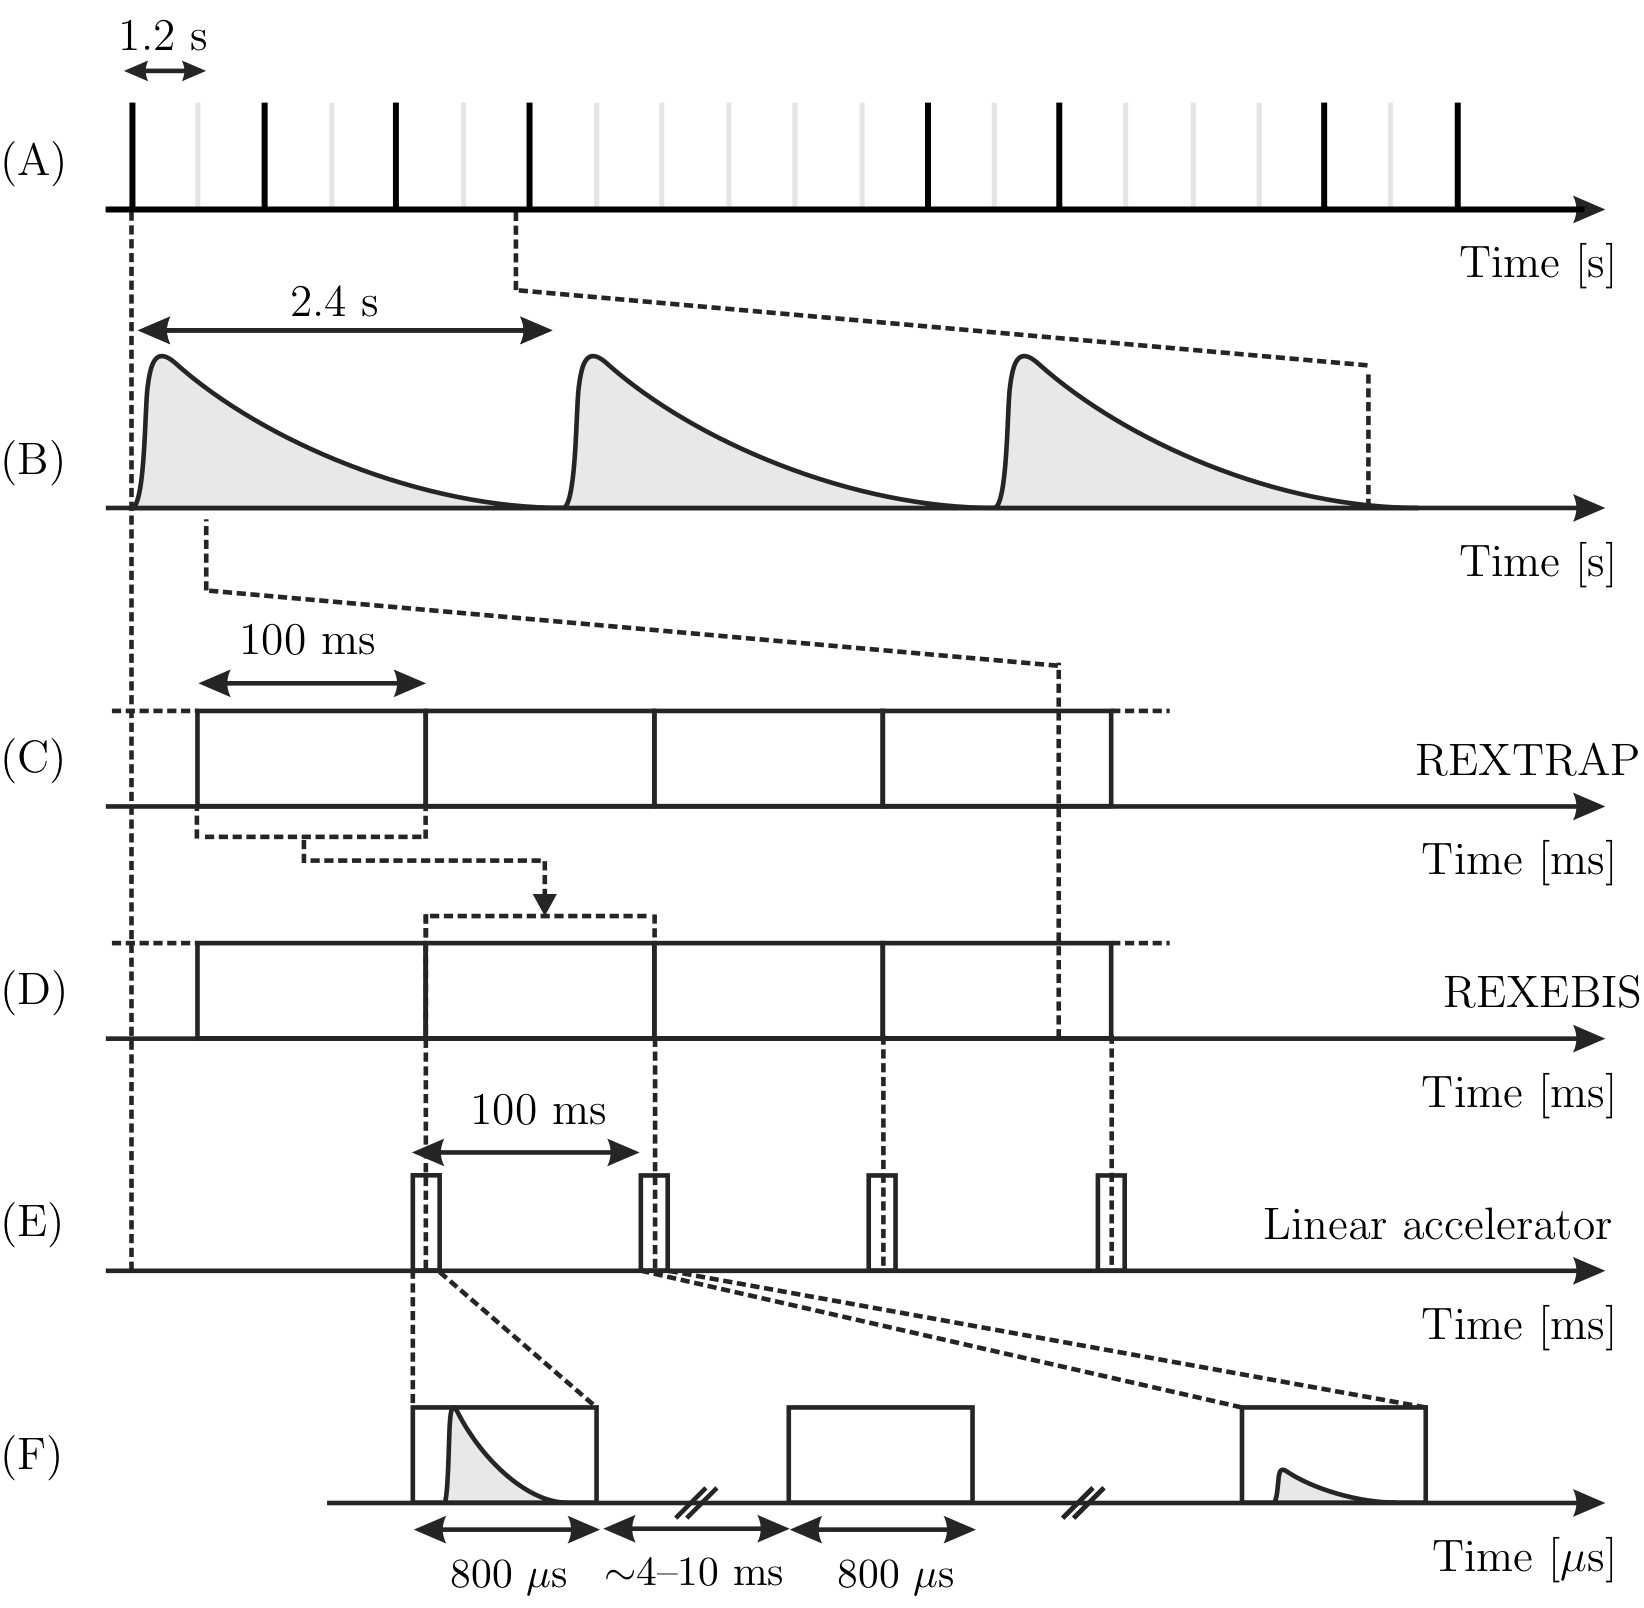
\includegraphics[width=\textwidth]{Images/Time-structure.png}
	\caption{Schematic of the ISOLDE time structure. (A) The supercycle of proton beam bunches with a width of $\approx 100 ~\mu$s from the PSB separated by 1.2 s. The black vertical lines shows an allocation of the the bunches which the ISOLDE production target receives, while the others are distributed to other experiments. (B) The release profile of radionuclides from the production target, which is heavily modulated by the PSB cycle. (C+D) REXTRAP and REXEBIS beam bunches, synchronized with (E) the radio frequency (RF) window of the HIE-ISOLDE LINAC. (F) The "on-beam" and "off-beam" time window of 800 $\mu$s using the Miniball setup. Figure courtesy of J. van de Walle \cite{HI-TDR}.}
	\label{fig:ITS}
\end{figure}


The purpose of the time calibration is to align the time spectra so that a prompt time gate can be set. In this way it is possible to correlate particles and \ga-rays. Using the \texttt{ParticlePlot.cpp} script, the ADC time offsets can be extracted by the following commands
\begin{lstlisting}[language=sh]
$ cd /Users/trondwj/GitHub/MasterThesis/Scripts/plotting
$ root
root [0] .L ParticlePlot.cpp++
root [1] check_ADC_time_offsets("setup_Sm.txt")
\end{lstlisting}
or they can be manually reached by
\begin{lstlisting}[language=sh]
$ cd /Users/trondwj/GitHub/MasterThesis/Sorted_data
$ root Sm_user-TreeBuilder-2019-06-20.root
root [1] new TBrowser()
\end{lstlisting}
and in the browser, the histograms named \textit{tdiff\_gp\_i} (where \textit{i} is a number between 0 and 3 implying quadrant 1 to 4) will lie in the \textit{.root}-file without a folder. \autoref{fig:ADC_dt} shows the time offsets for the CD. The peaks of these plots have the interesting x-axis value. Zooming into the peaks, it is very clear what value it is. These values are provided in the calibration file under ADC time offsets (ticks). These values can change depending on the amount of data sorted, so it is wise to double check them when more data is added to the file. After the peak values have been collected, they should be written into the calibration file. The time offsets of this experiment was the following
\begin{lstlisting}[language=sh]
# ADC time offsets (ticks)
adc_0.TimeOffset:  0
adc_1.TimeOffset:  -2
adc_2.TimeOffset:  -3
adc_3.TimeOffset:  5
\end{lstlisting}
After the software threshold and ADC time offsets are added to the calibration file, we must re-run the \texttt{Q4S.sh}-step with \texttt{TreeBuilder} and the updated calibration file.

\begin{figure}[ht]
	\centering
	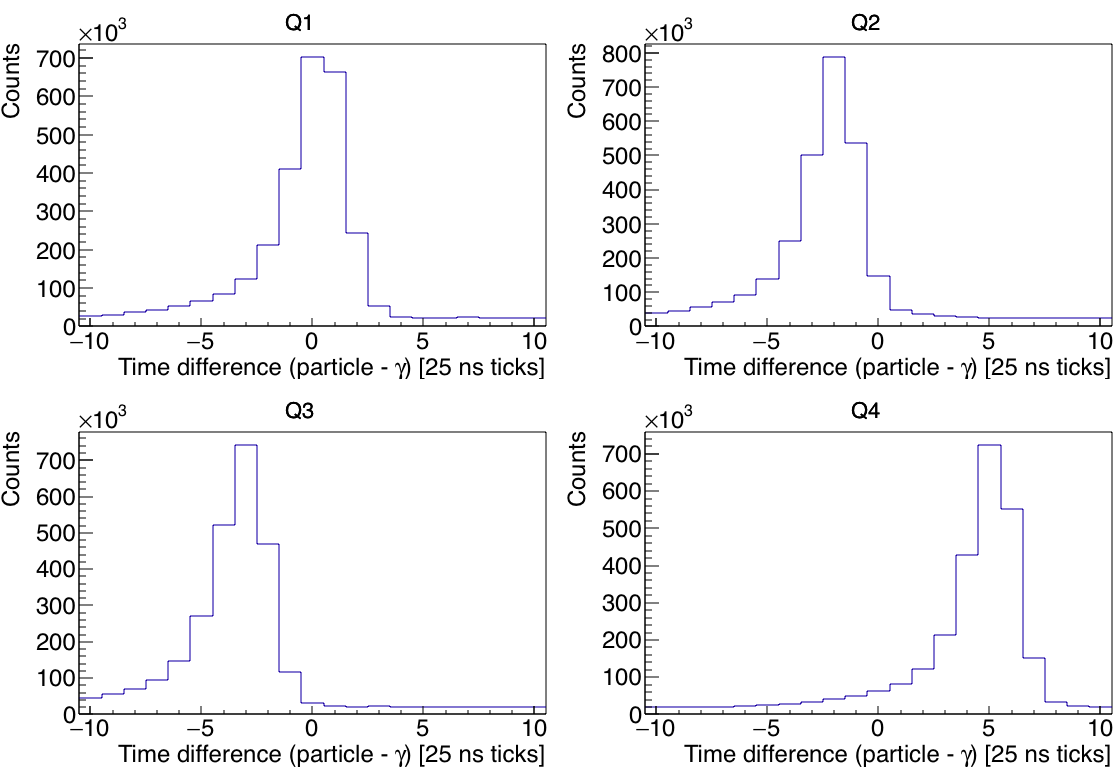
\includegraphics[width=\textwidth]{../Plots/plotting/tdiff_gp_0-3-user.png}
	\caption{ADC time offsets for the four quadrants of the CD.}
	\label{fig:ADC_dt}
\end{figure}



\subsection{Calibration of the \texorpdfstring{$\gamma$}{gamma} detectors}\label{sec:gamma}

The online calibration of the \ga\ detectors is quite good for most detectors in a certain energy range, because it is designed to be that way. 
During the setup of the experiment, a hardware calibration of the \ga\ detectors is performed. 
The gains of each DGF are matched so that the online analysis is more straightforward.
However, there are non-linearities and drifting offsets and gains over time that have to be corrected for with a proper calibration using the \Ba\ and \Eu\ source data collected in the end of the experiment. The \Ba\ and \Eu\ sources are placed at the target position simultaneously (back to back), and the data is also used to determine the relative efficiency of Miniball. 

\bigskip

E\_gam\_seg\_[0-7]\_[0-2]\_[0-6], cluster number (0-7), detector number (0-2) and segment number (0-6), where segment 0 is actually the core signal.

Gamma: \\
core ID from 0 to 23 \\
segment ID from 0 to 6 (zero is the core) \\
cluster ID from 0 to 7 \\

The thing with core ID 15 is a cross-talk issue involving a dead segment in detector 18A. It means that some events have to be vetoed to avoid double-peaking and this reduces the efficiency. You can see this list of vetoed detectors in Addback.hh line 193. In my most recent version, I am also vetoing segment number 106 for this reason.

\bigskip


\textcolor{red}{The \textit{-s} flag (singles) is for adding particles which come without a \ga-ray and the \textit{-addback} flag is for adding Compton scattered events together in the Miniball clusters.}

\textcolor{red}{\textbf{Then I have misunderstood the singles method?}}

There are three methods of sorting the events from Miniball; singles, add-back and reject. 
When applying the singles method, every \ga-ray entering a detector is counted as an event.
There are no assumptions of Compton scattering in this kind of sorting. 
This implies that some of the events counted as true events are in fact scattered \ga's corresponding to a different energy.
When utilizing the add-back method, events occurring in neighboring detectors in the same cluster within a 100 ns time window are added together as a single event. 
The energies of the events that occurred in the separate segments are summed, and the segment with the highest energy is assumed to be the position of the incident \ga-ray.
An advantage of the add-back method is that the full energy of a single \ga-ray, which has undergone a Compton scattering process, can be reconstructed to increase the efficiency.
A disadvantage of the method is the uncertainty in the assumptions of the addition of several events into a single event. 
The timing resolution cannot distinguish true \ga-\ga\ events from Compton scattering events.
The add-back method can cause an increase in the intensity of \ga-ray sum peaks since it has no way to deal with pile-up of different \ga-rays, thus no correction is performed when different \ga-rays pile up in the detector.
When applying the reject method for the sorting, events occurring in neighboring detectors in the same cluster within a 100 ns time window is excluded as an event. 
The total statistics for the reject method will therefore be smaller. 
If the amount of total statistics is large, it is possible and maybe even advantageous to apply the reject method, because it will give a higher probability of getting the actual full energy peaks of the \ga-rays detected. 




\bigskip




\textbf{CLXAna:}\newline
\begin{lstlisting}[language=]
-c: configuration file is a file that contains all of the parameters to save you typing them on the command line each time
-cut: the root file containing the graphical cuts on the kinematics (from the part histogram). This is the only thing you can't put in the above configuration file
-Ex: excitation energy of the state that you want to perform the Doppler correction for, in keV. Not significant, really.
-depth: depth of the interaction in the target. I usually assume half of the thickness, but you can test different values to see if it improves the Doppler correction.
-cdoffset: the rotation of the CD detector in the phi angle. Can be optimised, but is around 242.6 (default value).
-deadlayer: exactly as you say, this should be 0.7 um or 0.0007 mm (default value).
-spededist: not needed
-bg_frac: depends on the time windows defined in TreeBuilder, which means it should be -0.75 for the current version. This number can also be checked by taking the ratios of the beta-decay background peaks in the 'p' and 'r' spectra.
\end{lstlisting}

In the output file of CLXAna you will find a histogram called B\_dcB\_cid, which is the Doppler corrected spectra vs. each detector. The peak energies should of course be constant as a function of detector number, if they vary, then the angles need to be improved.

graphical cuts from the CLXAna-step (partQx) with Energy vs lab angle

After making the cut, right click and SetName to either "Bcut" or "Tcut". Then right click and SaveAs, giving the name of a root file of your choice (key is the \textit{.root} extension so that it knows which file format to use).

Do this for both the target-like (Tcut) and and beam-like (Bcut) particles. You will have one file each that you need to add together using 'hadd':

\begin{lstlisting}[language=]
hadd outputfile.root input1.root input2.root
\end{lstlisting}

What does the Bcut and Tcut indicate from [cutfile.root:Bcut:Tcut]?
Should the name have these? Are they values, names or other stuff?
This is the \textit{outputfile.root} that you just created in the last step, plus the names of the cuts in that file. The first cut is the beam-like and the second is the target-like. You can choose these names, but they must match the names that you set in the first step.

DGF: Digital \ga~ finder

addback, singles, ...


\begin{table}[ht] 
	\centering 
	\caption{DGF}
	% Data for the DGF table
\begin{tabular}{cccc}
\hline
Cluster & Detector & Segment & TreeBuilder            \\
\hline
0       & 0        & 0       & E\_gam\_seg\_0\_0\_0   \\
\hline
\end{tabular}
	\label{tab:DGF}
\end{table}


\subsubsection{CLXAna}
\begin{lstlisting}[language=]
$ ./Coulex.sh -n
--- Coulex: normal ---
Input parameters:
Zb = 62
Ab = 140
Zt = 82
At = 208
Eb = 4650 keV/u
Ex = 531 keV
thick = 1.4 mg/cm2
depth = 0.7 mg/cm2
cddist = 26.98 mm
cdoffset = 242.6 degrees
deadlayer = 0.0007 mm
contaminant = -1 mg/cm2
spededist = 23.6 mm
bg_frac = -0.75
srim = /Users/trondwj/GitHub/MasterThesis/SRIM
cutfile = ../../Sorted_data/outputfile.root:Bcut:Tcut
Begin g_clx loop.
Info in <TCanvas::Print>: pdf file /Users/trondwj/GitHub/MasterThesis/SRIM/140Sm_208Pb.pdf has been created
Info in <TCanvas::Print>: pdf file /Users/trondwj/GitHub/MasterThesis/SRIM/208Pb_208Pb.pdf has been created
Info in <TCanvas::Print>: pdf file /Users/trondwj/GitHub/MasterThesis/SRIM/140Sm_Si.pdf has been created
Info in <TCanvas::Print>: pdf file /Users/trondwj/GitHub/MasterThesis/SRIM/208Pb_Si.pdf has been created
Initialising histograms...
Looping over events...
Warning in <TClass::Init>: no dictionary for class trevts is available
1-particle events = 89020258%)    
Finished.
\end{lstlisting}


\subsubsection{hadd (from ROOT)}
After saving "part" from \texttt{CLXAna}-file:
\begin{lstlisting}[language=]
$ cd GitHub/ROOT-framework/build/bin
$ hadd /Users/trondwj/GitHub/MasterThesis/Sorted_data/outputfile.root /Users/trondwj/GitHub/MasterThesis/Sorted_data/part.root /Users/trondwj/GitHub/MasterThesis/Sorted_data/Bcut.root /Users/trondwj/GitHub/MasterThesis/Sorted_data/Tcut.root 
\end{lstlisting}

\bigskip


The Miniball spectrometer \cite{MB-spect} \newline
p. 8: \newline
\textbf{Efficiency and resolution:}
left bottom: \newline
The application of an add-back (AB) routine involves the summing of the energies of two coincident gamma rays within 100 ns in neighboring cores on the same cluster detector. This situation corresponds to a Compton-scattered \ga-ray event where the energy of the \ga-ray is shared between two or more crystals in the same triple cluster detector. For higher-energy \ga-rays, where scattering from one crystal into its neighbor is quite likely, this improves the efficiency, but for low-energy \ga-rays, where scattering is less likely, summing effects actually reduce the efficiency. For this reason a cut-off is normally applied and AB is only performed for energies above this threshold. \newline


\subsection{Doppler correction}

In order to perform the Doppler correction, the interaction point angles in the Miniball frame of reference has to be known. 
\autoref{fig:MB-angles} shows a sketch of the Miniball cluster geometry and \autoref{tab:Geo} gives the angles and distance of the different clusters.
The parameters $\theta$, $\phi$ and $R$ describes the position of the central axis of the detector clusters, while $\alpha$ describes the orientation about the axis of the cluster. All these parameters are needed to calculate the position of the segments or the position of a point determined by the pulse-shape analysis. 
The interaction point is determined either from the segment with the largest energy or using a pulse-shape analysis. 
In the first case, the position of the center of each segment has to be known.
In the second case, geometrical information to relate the time-to-steepest slope and ratio of the mirror charge amplitudes to the angle between the interaction point, the target and the emitted particle need to be known. 
This is built into \texttt{MiniballCoulexSort}, which does the geometrical calculations. 
The geometry parameters of the Miniball clusters has to be written into the calibration file. 

\begin{figure}[ht]
	\centering
	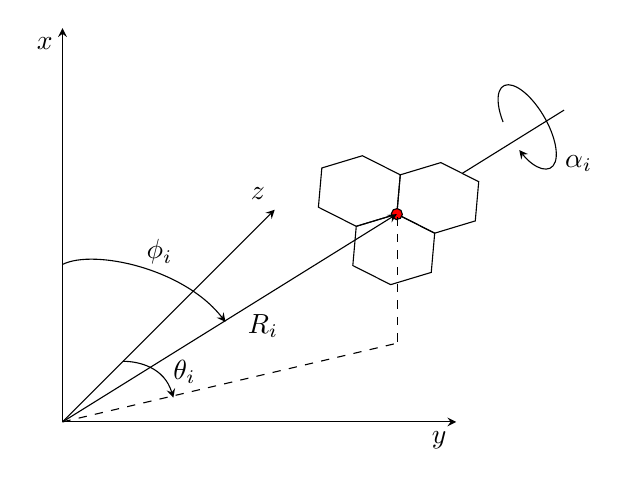
\begin{tikzpicture}
    % Definitions
    \coordinate (origo) at (0,0,0);
    % Coordinate system
    \draw[->,>=stealth] (origo) -- (5,0,0)  node[anchor=north east] {$y$};
    \draw[->,>=stealth] (origo) -- (0,5,0)  node[anchor=north east] {$x$};
    \draw[->,>=stealth] (origo) -- (0,0,-7) node[anchor=south east] {$z$};
    % Line following R
    \draw[>=stealth,rotate=-5] (4,3) -- (6,4.5);
    % HPGe
    \draw[rotate=-5,fill=white] (4,3) -- ++(0.5,-0.2) -- ++(0.5,0.2) -- ++(0,0.5) -- ++(-0.5,0.2) -- ++(-0.5,-0.2) -- cycle;
    \draw[rotate=-5] (3,3) -- ++(0.5,-0.2) -- ++(0.5,0.2) -- ++(0,0.5) -- ++(-0.5,0.2) -- ++(-0.5,-0.2) -- cycle;
    \draw[rotate=-5] (3.5,2.3) -- ++(0.5,-0.2) -- ++(0.5,0.2) -- ++(0,0.5) -- ++(-0.5,0.2) -- ++(-0.5,-0.2) -- cycle;
    % Red point in HPGe center
    \draw[fill=red,rotate=-5] (4,3) circle (2pt);
    % Distance vector
    \draw[->,>=stealth,rotate=-5] (origo) -- (4,3) node[anchor=north,pos=0.6,outer sep=1mm]
    {$R_i$};
    % Vector decomposition
    \draw[dashed] (origo)    -- (4.25,1);
    \draw[dashed] (4.25,2.6) -- (4.25,1);
    % Angles
    \draw[<-,x=0.25cm,y=0.60cm,>=stealth,rotate=30] (27,0.15) arc (-160:160:1 and 1) node[anchor=north west,pos=1.5] {$\alpha_i$};
    \draw[->,>=stealth] (0,0,-2) .. controls (0.2,0,-2) and (0.6,0,-1.8)   .. (1.1,0,-0.8) node[anchor=west,pos=0.6,outer sep=1mm] {$\theta_i$};
    \draw[->,>=stealth] (0,2,0) .. controls (0.4,2.2,0) and (0.7,1.1,-2.2) .. (1.3,0.5,-2) node[above,pos=0.6] {$\phi_i$};
\end{tikzpicture}
	\caption{Miniball angles, where $i$ denotes cluster number from \autoref{tab:Geo} and the $z$-axis is the beam direction. The angles ($\theta$ and $\phi$) are defined from a right-hand polar coordinate system, while the angle $\alpha$ determines the clockwise rotation around the center of the triple-cluster as seen from the target position \cite{NWarr-Angles}.}
	\label{fig:MB-angles}
\end{figure}


\begin{table}[ht] 
	\centering 
	\caption{Geometry to the center of the Miniball HPGe clusters (red dot in \autoref{fig:MB-angles}) for the Doppler correction.}
	% Data for the Geometry table
\caption{Geometry}
\label{tab:Geo}
\begin{tabular}{ccccc}
\hline
Cluster  &  $\theta$ [$^\circ$]  &  $\phi$ [$^\circ$]  &  $\alpha$ [$^\circ$]  &  R [mm]  \\
\hline
0        &  311.16               &  126.67             &  129.79               &  107.08  \\
1        &  51.08                &  62.74              &  51.83                &  100.59  \\
2        &  309.02               &  126.87             &  51.23                &  105.76  \\
3        &  251.90               &  57.44              &  130.31               &  105.40  \\
4        &  296.93               &  235.53             &  128.74               &  106.48  \\
5        &  233.45               &  239.09             &  46.67                &  105.18  \\
6        &  59.42                &  308.67             &  131.04               &  127.04  \\
7        &  130.56               &  309.09             &  46.46                &  110.18  \\
\hline
\end{tabular}

	\label{tab:Geo}
\end{table}




Because of the significant velocity of the scattered particles, the emitted \ga-rays from the particle de-excitation has a Doppler shifted \ga-energy given by 
\begin{equation}\label{eq:DS}
	E_\gamma = \frac{E_\gamma^{'}}{\gamma (1 - \beta \cos \theta)}
\end{equation}
where $E_\gamma$ is the \ga-energy detected in the LAB frame, $E_\gamma^{'}$ is the \ga-energy in the nucleus' frame of reference, $\beta = \frac{v}{c}$, $v$ is the nucleus' velocity, $c$ is the speed of light, $\theta$ is the angle of the emitted \ga-ray with respect to the nucleus' direction of motion and $\gamma = 1/\sqrt{1 - \beta^2}$ is the Lorentz factor. Since both the CD and the HPGe-array are segmented, the emission angle $\theta$ of the \ga-ray can be calculated by 
\begin{equation}\label{eq:DSA}
	\cos \theta = \sin \theta_p \sin \theta_\gamma \cos (\phi_p - \phi_\gamma) + \cos \theta_p \cos \theta_\gamma
\end{equation}
where ($\theta_p, \phi_p$) and ($\theta_\gamma, \phi_\gamma$) are the detection angles of the particle and \ga-ray respectively, ($\theta_p, \theta_\gamma$) are the angles with respect to the beam axis and ($\phi_p, \phi_\gamma$) are the azimuthal angles \cite{RIBF2012, MB-spect}. The Doppler correction factor is found by combining \autoref{eq:DS} and \autoref{eq:DSA} into
\begin{equation}
	\frac{E_\gamma^{'}}{E_\gamma} = \gamma (1 - \beta (\sin \theta_p \sin \theta_\gamma \cos (\phi_p - \phi_\gamma) + \cos \theta_p \cos \theta_\gamma))
\end{equation}


\subsection{Broken detector segments}

CD: ring 1 + Quadrant 4, front ring 16, back strip 1 \newline

\autoref{fig:BDS_B1} shows one pixel where back strip 1 (B1) is acting weird compared to the other back strips. There are other rings where B1 is a bit off, but not nearly as much as in this pixel. Maybe B1 should be excluded, but in this thesis, it was used. 

\bigskip

HPGe: Core ID 20? Other? Check vetoed segments


\begin{figure}[ht]
	\centering
	\begin{subfigure}{\textwidth}
		\centering
		% plot_quadrants("setup_Sm.txt", "f", 1, 0, 1, 0, 3500, 8500)
		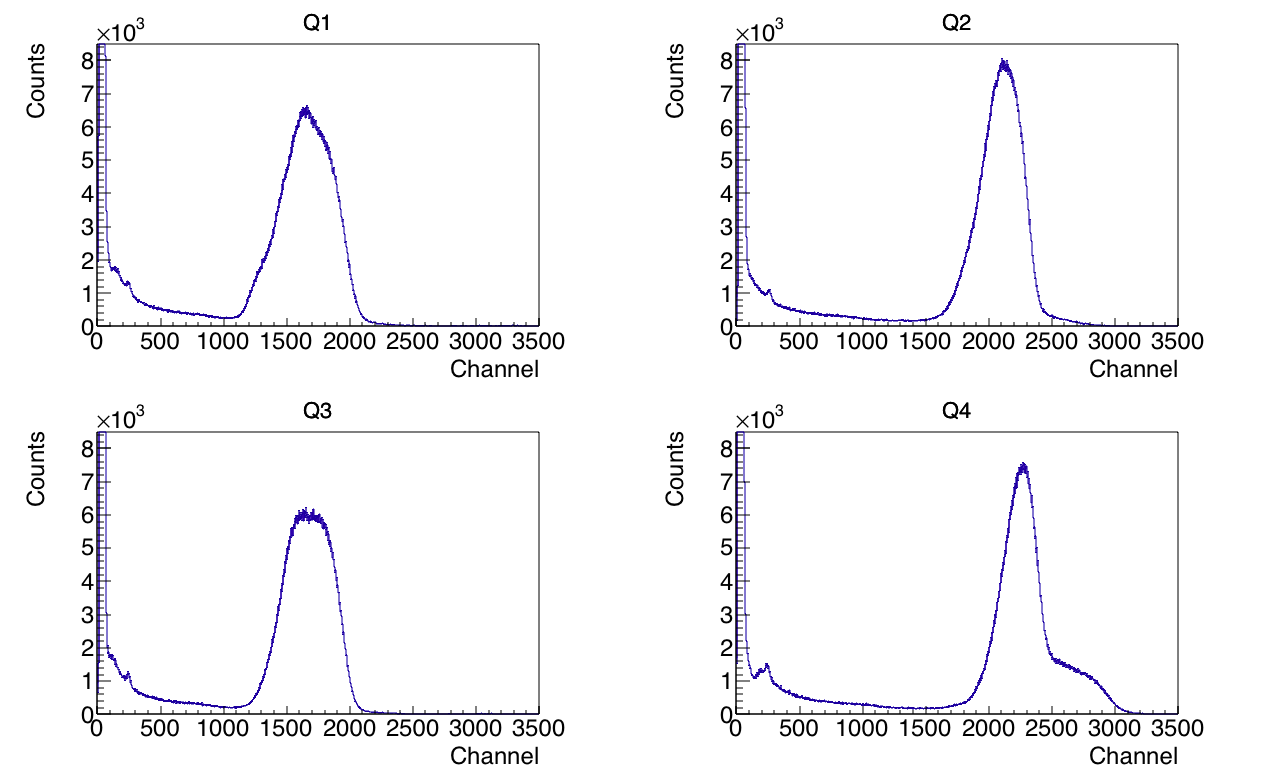
\includegraphics[width=\textwidth]{../Plots/plotting/Q1-4_f1.png}
		\caption{CD front ring 1 (innermost ring).}
		\label{fig:BDS_R1}
	\end{subfigure}
	\begin{subfigure}{\textwidth}
		\centering
		% plot_back_strips("setup_Sm.txt", 4, 16, 0, 0, 1700, 400)
		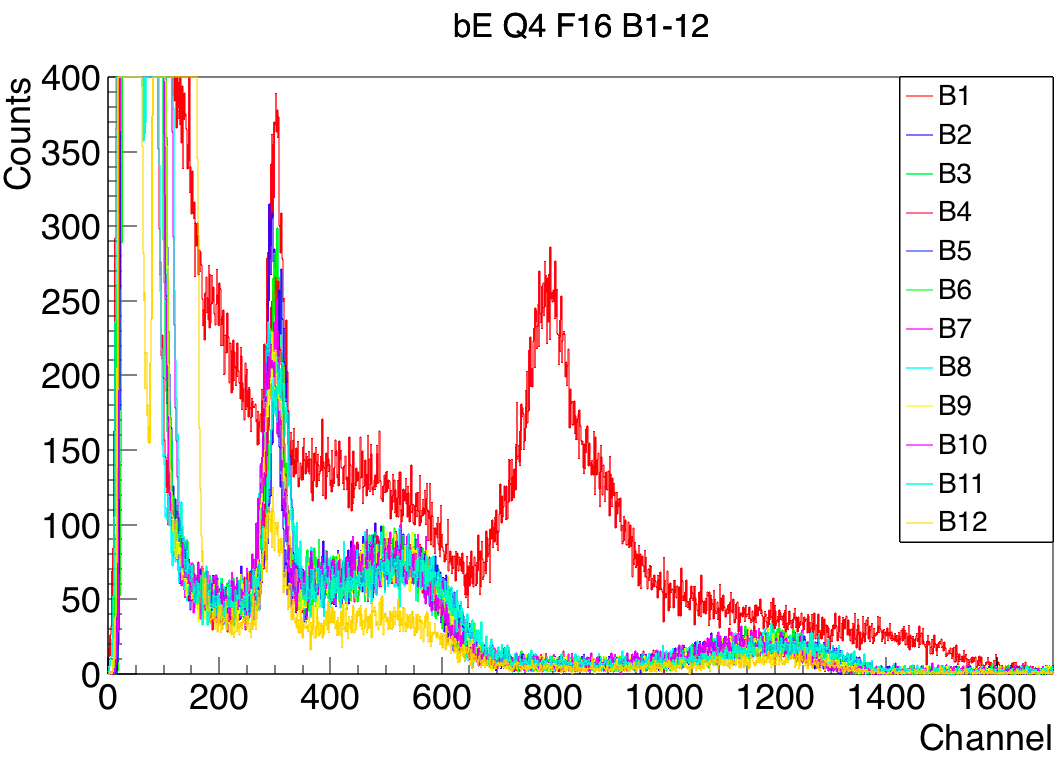
\includegraphics[width=\textwidth]{../Plots/plotting/bE_Q4_f16_b1-12.png}
		\caption{CD back strip 1 gated on front ring 16 (outermost ring) in quadrant 4.}
		\label{fig:BDS_B1}
	\end{subfigure}
	\caption{LAB vs. CM frame.}
	\label{fig:BDS}
\end{figure}


% ----------------------------------------------------------------------------------------------------------------------% ----------------------------------------------------------------------------------------------------------------------


\chapter{Experimental results and discussion}


Very pure beam (\textcolor{red}{did we have statistics of this?}) - resultat til avhandling. sjekk etter doppler-korrigering. Nd-contaminasjon? i så fall veldig lite, 1-2 prosent?

\textcolor{Magenta}{Tilbakemelding: \newline
we would have to look at the \ga-spectra to identify any contaminants. There may be a little bit of Nd-140 in the beam, but if so, it is very little (judging from on-line spectra).}


\bigskip


Level scheme (from Klintefjord?)\newline

\textcolor{Magenta}{Tilbakemelding: \newline
at some point you should show the level scheme. \newline
$\bullet$ motivation: to explain what is known, and which transition probabilities you want to measure.  \newline
Perhaps also to explain what theory predicts. \newline
$\bullet$ discussion: if you get \ga-spectrum for \Sm\ $\rightarrow$ to explain what you see.}


\begin{figure}[ht]
	\centering
	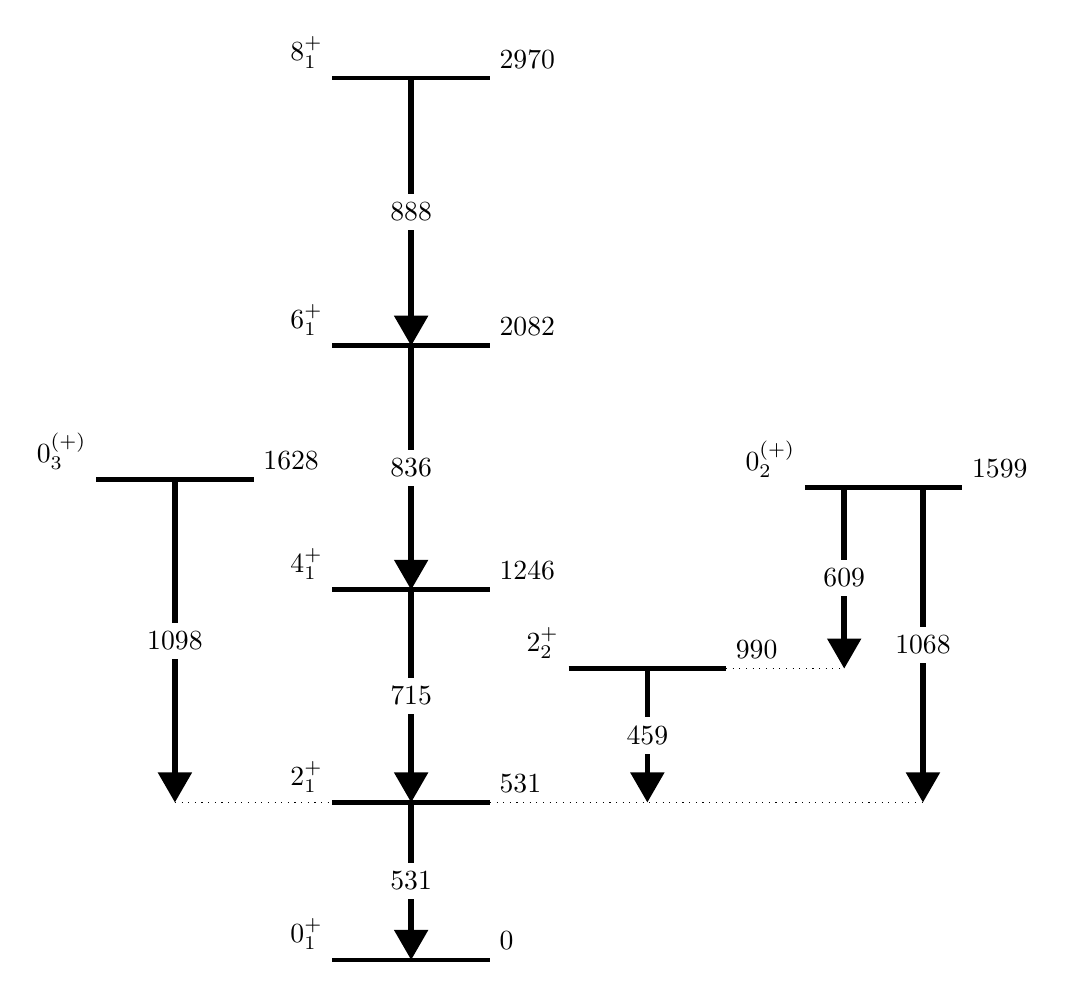
\begin{tikzpicture}[
    level/.style = { ultra thick, black },
    connect/.style = { dotted, black },
    notice/.style = { draw, rectangle callout, callout relative pointer={#1} },
    label/.style = { text width=2cm }
    ]
    %%% Picture made by normalizing energy to the 2+ state (531) and choosing it to be 
    %%% 2 units of y in height.

    %%%
    %%% Ground state band
    %%%
    % Levels, states, energy
    \foreach \level / \state / \energy in {0/0_1^+/0, 2/2_1^+/531, 4.7/4_1^+/1246, 7.8/6_1^+/2082, 11.2/8_1^+/2970}
      { 
        \draw[level] (0,\level) -- (2,\level);
        \node at (0,\level) [anchor=south east] {$\state$};
        \node at (2,\level) [anchor=south west] {$\energy$};
      }
    % Gamma transitions
    \foreach \endlevel / \startlevel / \gamma in {0/2/531, 2/4.7/715, 4.7/7.8/836, 7.8/11.2/888}
      { 
        \draw[line width=2pt, ->, >=triangle 60] (1,\startlevel) -- node[fill=white] {\gamma} (1,\endlevel);
      }
    % Dotted lines
    \draw[connect] (-2,2) -- (0,2) (2,2) -- (7.5,2);
    %\draw[connect] (-2,11.2) -- (0,11.2) (2,11.2) -- (4,11.2);
    
    %%%
    %%% Left band
    %%%
    % Lower left band
    \coordinate (levelleft)  at (-3,6.1);
    \coordinate (levelright) at (-1,6.1);
    \draw[level] (levelleft) -- (levelright);
    \node at (levelleft)  [anchor=south east] {$0_3^{(+)}$};
    \node at (levelright) [anchor=south west] {1628};
    \draw[line width=2pt, ->, >=triangle 60] (-2,6.1) -- node[fill=white] {1098} (-2,2);
    %% Higher left band
    %\foreach \level / \state / \energy in {12.1/10^+/3211, 13.8/12^+/3653, 16.6/14^+/4404, 20.3/16^+/5398}
    %  { 
    %    \draw[level] (-3,\level) -- (-1,\level);
    %    \node at (-3,\level) [anchor=south east] {$\state$};
    %    \node at (-1,\level) [anchor=south west] {$\energy$};
    %  }
    %% Gamma transitions
    %\foreach \endlevel / \startlevel / \gamma in {12.1/13.8/442, 13.8/16.6/751, 16.6/20.3/994}
    %  { 
    %    \draw[line width=2pt, ->, >=triangle 60] (-2,\startlevel) -- node[fill=white] {\gamma} (-2,\endlevel);
    %  }
    %% First gamma transition
    %\draw[line width=2pt, ->, >=triangle 60] (-2,12.1) -- node[left=3pt] {241} (-2,11.2);

    %%%
    %%% 1st right band
    %%%
    % Lower 1st right band
    \coordinate (levelleft)  at (3,3.7);
    \coordinate (levelright) at (5,3.7);
    \draw[level] (levelleft) -- (levelright);
    \node at (levelleft)  [anchor=south east] {$2_2^+$};
    \node at (levelright) [anchor=south west] {990};
    \draw[line width=2pt, ->, >=triangle 60] (4,3.7) -- node[fill=white] {459} (4,2);
    % Dotted lines
    \draw[connect] (levelright) -- (6.5,3.7);
    %% Higher 1st right band; levels, states, energy
    %\foreach \level / \state / \energy in {11.9/10^+/3172, 14.3/12^+/3791, 18.5/14^+/4914}
    %  { 
    %    \draw[level] (3,\level) -- (5,\level);
    %    \node at (3,\level) [anchor=south east] {$\state$};
    %    \node at (5,\level) [anchor=south west] {$\energy$};
    %  }
    %% Gamma transitions
    %\foreach \endlevel / \startlevel / \gamma in {11.9/14.3/619, 14.3/18.5/1123}
    %  { 
    %    \draw[line width=2pt, ->, >=triangle 60] (4,\startlevel) -- node[fill=white] {\gamma} (4,\endlevel);
    %  }
    %% First gamma transition
    %\draw[line width=2pt, ->, >=triangle 60] (4,11.9) -- node[right=4pt] {202} (4,11.2);

    %%%
    %%% 2nd right band
    %%%
    \coordinate (levelleft)  at (6,6);
    \coordinate (levelright) at (8,6);
    \draw[level] (levelleft) -- (levelright);
    \node at (levelleft)  [anchor=south east] {$0_2^{(+)}$};
    \node at (levelright) [anchor=south west] {1599};
    \draw[line width=2pt, ->, >=triangle 60] (7.5,6) -- node[fill=white] {1068} (7.5,2);
    \draw[line width=2pt, ->, >=triangle 60] (6.5,6) -- node[fill=white] {609} (6.5,3.7);    
\end{tikzpicture}
	\caption{Level scheme for \Sm. Adapted from Klintefjord.}
	\label{fig:levels}
\end{figure}




% ----------------------------------------------------------------------------------------------------------------------% ----------------------------------------------------------------------------------------------------------------------

\chapter{Summary and outlook}

Future work: Better calibration of particle detectors and \ga-detectors (online not perfect). Take into account the shape of the peaks $\implies$ calibrate the particle detectors manually.. Takes a lot of time! But maybe less than trying to fit all in a script? If someone only knew and told this story...

Use a second opinion on the simulation, maybe try LISE++ or some other simulation program to get the centroids?
Maybe \texttt{kinsim3} uses too much energy loss in CD? 
If you are using only the Pb and Sm for calibration, and then applying that calibration back to the data, then it should matter if the absolute energies are correct. 
This is an internal calibration, so that would simply mean that the peaks would have the wrong energy, but they should still be aligned on the front and back.

\bigskip

Efficiency calibration ++

\bigskip

\textcolor{red}{Fra oppgaveteksten:} \newline
determine Coulomb excitation yields. These yields will then, in a second step, be compared to theoretical calculations and transition probabilities and quadrupole moments will be extracted using chi-square minimization procedures.


GOSIA and GOSIA2 analysis?

\url{https://www.pas.rochester.edu/~cline/Gosia/Gosia_Manual_20110609.pdf}

% ----------------------------------------------------------------------------------------------------------------------% ----------------------------------------------------------------------------------------------------------------------




% ----------------------------------------------------------------------------------------------------------------------% ----------------------------------------------------------------------------------------------------------------------

\begin{appendices}

\chapter{Acronyms and abbreviations}

\begin{table}[ht] 
	\centering 
	%\caption{Table of acronyms and abbreviations.}
	% Data for the Acronyms and abbreviations table
\begin{tabular}{ll}
    \hline
    ADC         &  Analog to Digital Converter                                \\
    bash        &  Bourne-Again SHell                                         \\
    CERN        &  European Council for Nuclear Research                      \\ 
                &  (in French: Conseil Européen pour la Recherche Nucléaire)  \\
    CD          &  Compact Disc                                               \\
    COULEX      &  COULomb EXcitation                                         \\
    DAQ         &  Data AcQuisition                                           \\
    DGF         &  Digital Gamma Finder                                       \\
    DSSSD       &  Double Sided Silicon Strip Detector (also known as CD)     \\
    GPS         &  General Purpose Separator                                  \\
    HRS         &  High Resolution Separator                                  \\
    HIE-ISOLDE  &  High Intensity and Energy upgrade at ISOLDE                \\
    HPGe        &  High Purity Germanium                                      \\
    ISOL        &  Isotope Separator On Line                                  \\
    ISOLDE      &  ISOL DEvice                                                \\
    LINAC       &  LINear ACcelerator                                         \\
    MBS         &  Multi Branch System                                        \\
    MED         &  MBS Event Data (also known as Miniball Event Data)         \\
    MAR\belowbaseline[-2pt]{a}B\stackinset{l}{3pt}{b}{-3pt}{O}{O}\,U     
                &  MBS And ROOT Based Online/Offline Utility                  \\
    PSB         &  Proton Synchrotron Booster                                 \\
    REX         &  Radioactive beam EXperiment                                \\
    EBIS        &  Electron Beam Ion Source                                   \\
    REXEBIS     &  Radioactive beam EXperiment Electron Beam Ion Source       \\
    REXTRAP     &  Radioactive beam EXperiment TRAP                           \\
    REX-ISOLDE  &  Radioactive beam EXperiment at ISOLDE                      \\
    RIB         &  Radioactive Ion Beam                                       \\
    RILIS       &  Resonance Ionization Laser Ion Source                      \\
    SRIM        &  Stopping and Range of Ions in Matter                       \\
    TDC         &  Time to Digital Converter                                  \\
    \hline
\end{tabular}
\label{tab:acro}

	\label{tab:acro}
\end{table}


% ----------------------------------------------------------------------------------------------------------------------% ----------------------------------------------------------------------------------------------------------------------

\chapter{Symbol list}

\begin{table}[ht]
  \centering
  \caption{Table of symbols with explanations.}
    \begin{tabular}{ll}
        \hline
        T$_{1/2}$ & Half-life \\
        \hline
    \end{tabular}
    \label{tab:symbols}
\end{table}

% ----------------------------------------------------------------------------------------------------------------------% ----------------------------------------------------------------------------------------------------------------------

\chapter{Two-particle collision}
\section{Laboratory (LAB) frame of reference}\label{sec:LAB}
The angles of the two-particle collision in the laboratory frame from \autoref{fig:LAB} is calculated in this section. A general approach is used to make it easier to hold track of the parameters. From the figure we can express the velocities as
\begin{align}\label{eq:2p-LAB-collision}
\begin{split}
	 \boldsymbol{u} &= \boldsymbol{u}_1 = u \boldsymbol{\hat{x}}  \\
	 \boldsymbol{u}_2 &= 0  \\
	 \boldsymbol{v}_b &= \boldsymbol{v}_1 = v_1 (\cos \theta \boldsymbol{\hat{x}} + \sin \theta \boldsymbol{\hat{y}})  \\
	\boldsymbol{v}_t &= \boldsymbol{v}_2 = v_2 (\cos \varphi \boldsymbol{\hat{x}} - \sin \varphi \boldsymbol{\hat{y}})
\end{split}
\end{align}
where $\boldsymbol{u}_1$ and $\boldsymbol{v}_1$ is the initial and final velocity of the projectile $m_b = m_1$ respectively, and $\boldsymbol{u}_2$ and $\boldsymbol{v}_2$ is the initial and final velocity of the target $m_t = m_2$ respectively. The angles $\theta_b = \theta$ and $\theta_t = \varphi$ are the projectile and target angle respectively. We also introduce a ratio of the projectile mass to the target mass, $\alpha = m_1/m_2$.

Conservation of momentum gives
\begin{align*}%\label{eq:comom}
	m_1 \boldsymbol{u}_1 &= m_1 \boldsymbol{v}_1 + m_2 \boldsymbol{v}_2
\end{align*}
which in x-direction can be expressed as
\begin{align}\label{eq:comx}
	m_1 u &= m_1 v_1 \cos \theta + m_2 v_2 \cos \varphi  \nonumber\\
	m_1 (u - v_1 \cos \theta) &= m_2 v_2 \cos \varphi  \nonumber\\
	\frac{m_1}{m_2} (u - v_1 \cos \theta) &= v_2 \cos \varphi  \nonumber\\
	\alpha (u - v_1 \cos \theta) &= v_2 \cos \varphi
\end{align}
and in y-direction can be expressed as
\begin{align}\label{eq:comy}
	0 &= m_1 v_1 \sin \theta - m_2 v_2 \sin \varphi \nonumber\\
	m_1 v_1 \sin \theta &= m_2 v_2 \sin \varphi \nonumber\\
	\frac{m_1}{m_2} v_1 \sin \theta &= v_2 \sin \varphi \nonumber\\
	\alpha v_1 \sin \theta &= v_2 \sin \varphi
\end{align}

Conservation of energy gives
\begin{align}\label{eq:coe}
	\tfrac{1}{2} m_1 \boldsymbol{u}_1^2 &= \tfrac{1}{2} m_1 \boldsymbol{v}_1^2 + \tfrac{1}{2} m_2 \boldsymbol{v}_2^2 \nonumber\\
	\tfrac{1}{2} m_1 (u^2 - v_1^2) &= \tfrac{1}{2} m_2 v_2^2 \nonumber\\
	\frac{m_1}{m_2} (u^2 - v_1^2) &= v_2^2 \nonumber\\
	\alpha (u^2 - v_1^2) &= v_2^2
\end{align}

We now have three equations (\autoref{eq:comx} - \autoref{eq:coe}) with four unknown quantities ($v_1, \theta, v_2, \varphi$). Using the target angle $\varphi$ as an independent variable, we can find expressions for the other three variables. 

Squaring \autoref{eq:comx} 
\begin{align*}%\label{eq:c}
	\alpha^2 (u - v_1 \cos \theta)^2 &= v_2^2 \cos^2 \varphi  \\
	\alpha^2 (u^2 - 2uv_1 \cos \theta + v_1^2 \cos^2 \theta) &= v_2^2 \cos^2 \varphi
\end{align*}
and \autoref{eq:comy}
\begin{align*}%\label{eq:c}
	\alpha^2 v_1^2 \sin^2 \theta &= v_2^2 \sin^2 \varphi
\end{align*}
and adding them together gives
\begin{align}\label{eq:av}
	\alpha^2 (u^2 - 2uv_1 \cos \theta + v_1^2 \cos^2 \theta + v_1^2 \sin^2 \theta) &= v_2^2 (\cos^2 \varphi + \sin^2 \varphi)  \nonumber\\
	\alpha^2 (u^2 - 2uv_1 \cos \theta + v_1^2) &= v_2^2  \nonumber\\
	\alpha^2 u^2 - 2\alpha^2 uv_1 \cos \theta + \alpha^2 v_1^2 &= v_2^2  \nonumber\\
	\alpha^2 v_1^2 &= -\alpha^2 u^2 + 2\alpha^2 uv_1 \cos \theta + v_2^2  \nonumber\\
	\alpha^2 v_1^2 &= -\alpha^2 u^2 + 2\alpha u (\alpha v_1 \cos \theta) + v_2^2
\end{align}
From \autoref{eq:comx} we have
\begin{align}\label{eq:comx2}
	\alpha (u - v_1 \cos \theta) &= v_2 \cos \varphi  \nonumber\\
	\alpha u - \alpha v_1 \cos \theta &= v_2 \cos \varphi  \nonumber\\
	\alpha v_1 \cos \theta &= \alpha u - v_2 \cos \varphi
\end{align}
Substituting for \autoref{eq:comx2} into \autoref{eq:av} we get
\begin{align}\label{eq:comsq}
	\alpha^2 v_1^2 &= -\alpha^2 u^2 + 2\alpha u (\alpha u - v_2 \cos \varphi ) + v_2^2  \nonumber\\
	\alpha^2 v_1^2 &= -\alpha^2 u^2 + 2\alpha^2 u^2 - 2\alpha u v_2 \cos \varphi + v_2^2  \nonumber\\
	\alpha^2 v_1^2 &= \alpha^2 u^2 - 2\alpha u v_2 \cos \varphi + v_2^2
\end{align}
Using \autoref{eq:coe} we get
\begin{align}\label{eq:coesub}
    \left( \frac{\alpha}{\alpha} \right) \alpha (u^2 - v_1^2) &= v_2^2  \nonumber\\
    \alpha^2 (u^2 - v_1^2) &= \alpha v_2^2  \nonumber\\
	\alpha^2 u^2 - \alpha^2 v_1^2 &= \alpha v_2^2  \nonumber\\
	\alpha^2 v_1^2 &= \alpha^2 u^2 - \alpha v_2^2
\end{align}
Combining \autoref{eq:comsq} and \autoref{eq:coesub} gives
\begin{align}\label{eq:comcoe}
    \alpha^2 u^2 - 2\alpha u v_2 \cos \varphi + v_2^2 &= \alpha^2 u^2 - \alpha v_2^2  \nonumber\\
    v_2^2 + \alpha v_2^2 &= 2\alpha u v_2 \cos \varphi  \nonumber\\
    v_2^2 (1 + \alpha) &= 2\alpha u v_2 \cos \varphi  \nonumber\\
    v_2 &= 2 \left( \frac{\alpha}{1 + \alpha} \right) u \cos \varphi 
\end{align}
Substituting \autoref{eq:comcoe} into \autoref{eq:coesub} we get
\begin{align}\label{eq:coesubsub}
    \alpha^2 v_1^2 &= \alpha^2 u^2 - \alpha \left( 2 \left( \frac{\alpha}{1 + \alpha} \right) u \cos \varphi  \right)^2  \nonumber\\
    v_1^2 &= u^2 - \frac{1}{\alpha} \left( 4 \left( \frac{\alpha^2}{(1 + \alpha)^2} \right) u^2 \cos^2 \varphi  \right)  \nonumber\\
    v_1^2 &= u^2 \left(1 - 4 \left( \frac{\alpha}{(1 + \alpha)^2} \right) \cos^2 \varphi  \right)  \nonumber\\
    v_1 &= u \sqrt{1 - 4 \frac{\alpha}{M} \cos^2 \varphi}
\end{align}
where $\alpha/M = \alpha/(1 + \alpha)^2$. The ratio of \autoref{eq:comy} and \autoref{eq:comx2} gives
\begin{align}\label{eq:comxy}
	\frac{\alpha v_1 \sin \theta}{\alpha v_1 \cos \theta} &= \frac{v_2 \sin \varphi}{\alpha u - v_2 \cos \varphi}  \nonumber\\
	\tan \theta &= \frac{v_2 \sin \varphi}{\alpha u - v_2 \cos \varphi}
\end{align}
Inserting \autoref{eq:comcoe} into \autoref{eq:comxy} gives
\begin{align}\label{eq:tanBgen}
	\tan \theta &= \frac{\left( 2 \left( \frac{\alpha}{1 + \alpha} \right) u \cos \varphi  \right) \sin \varphi}{\alpha u - \left( 2 \left( \frac{\alpha}{1 + \alpha} \right) u \cos \varphi  \right) \cos \varphi}  \nonumber\\
	\tan \theta &= \frac{\alpha u \left( \frac{1}{1 + \alpha} \right) 2 \sin \varphi \cos \varphi}{\alpha u \left(1 - 2 \left( \frac{1}{1 + \alpha} \right) \cos^2 \varphi \right)}  \nonumber\\
	\tan \theta &= \frac{\sin 2\varphi}{(1 + \alpha)\left(1 - 2 \left( \frac{1}{1 + \alpha} \right) \cos^2 \varphi \right)}  \nonumber\\
	\tan \theta &= \frac{\sin 2\varphi}{1 + \alpha - 2 \cos^2 \varphi}  \nonumber\\
	\tan \theta &= \frac{\sin 2\varphi}{\alpha - (2 \cos^2 \varphi - 1)}  \nonumber\\
	\tan \theta &= \frac{\sin 2\varphi}{\alpha - \cos 2\varphi}  \nonumber\\
	\theta &= \arctan \left( \frac{\sin 2\varphi}{\alpha - \cos 2\varphi} \right)
\end{align}
Substituting back the variable names from \autoref{fig:LAB} into \autoref{eq:tanBgen} gives
\begin{align}\label{eq:tanB}
	\theta_b &= \arctan \left( \frac{\sin 2\theta_t}{\alpha - \cos 2\theta_t} \right)
\end{align}


\section{Center of mass (CM) frame of reference}
Using the same approach as \autoref{sec:LAB}. From figure \autoref{fig:CM} we can express the velocities as
\begin{align}\label{eq:2p-CM-collision}
\begin{split}
	 \boldsymbol{u}_1^{'} &= u_1^{'} \boldsymbol{\hat{x}} \\
	 \boldsymbol{u}_2^{'} &= u_2^{'} \boldsymbol{\hat{x}} \\
	 \boldsymbol{v}_b^{'} &= \boldsymbol{v}_1^{'} = v_1^{'} (\cos \theta^{'} \boldsymbol{\hat{x}} + \sin \theta^{'} \boldsymbol{\hat{y}}) \\
	\boldsymbol{v}_t^{'} &= \boldsymbol{v}_2^{'} = v_2^{'} (-\cos \theta^{'} \boldsymbol{\hat{x}} - \sin \theta^{'} \boldsymbol{\hat{y}}) = -v_2^{'} (\cos \theta^{'} \boldsymbol{\hat{x}} + \sin \theta^{'} \boldsymbol{\hat{y}})
\end{split}
\end{align}
where $\boldsymbol{u}_1^{'}$ and $\boldsymbol{v}_1^{'}$ is the initial and final velocity of the projectile $m_b = m_1$ respectively, and $\boldsymbol{u}_2^{'}$ and $\boldsymbol{v}_2^{'}$ is the initial and final velocity of the target $m_t = m_2$ respectively. The angle $\theta_b^{'} = \theta^{'}$ is the projectile angle. 

In the center of mass (CM) frame of reference, the position of the center of mass is given by
\begin{align}\label{eq:CMpos}
	\boldsymbol{R} &= \frac{m_1 \boldsymbol{r}_1 + m_2 \boldsymbol{r}_2}{m_1 + m_2}
\end{align}
and the velocity is
\begin{align}\label{eq:Vcm}
	\boldsymbol{V} &= \frac{d\boldsymbol{R}}{dt}
	= \frac{d}{dt} \left( \frac{m_1 \boldsymbol{r}_1 + m_2 \boldsymbol{r}_2}{m_1 + m_2} \right)
	= \frac{m_1 \boldsymbol{u}_1^{'} + m_2 \boldsymbol{u}_2^{'}}{m_1 + m_2}
\end{align}
At the origin of the CM frame, $\boldsymbol{R} = 0$, which implies $\boldsymbol{V} = 0$. The total momentum before the collision is
\begin{align}\label{eq:ucm}
	m_1 \boldsymbol{u}_1^{'} + m_2 \boldsymbol{u}_2^{'} &= 0  \nonumber\\
	m_2 u_2^{'} &= -m_1 u_1^{'} \nonumber\\
	u_2^{'} &= - \frac{m_1}{m_2} u_1^{'} \nonumber\\
	u_2^{'} &= - \alpha u_1^{'}
\end{align}
and after the collision it is
\begin{align}\label{eq:vcm}
	m_1 \boldsymbol{v}_1^{'} + m_2 \boldsymbol{v}_2^{'} &= 0  \nonumber\\
	m_2 \boldsymbol{v}_2^{'} &= -m_1 \boldsymbol{v}_1^{'} \nonumber\\
	\boldsymbol{v}_2^{'} &= - \frac{m_1}{m_2} \boldsymbol{v}_1^{'} \nonumber\\
	\boldsymbol{v}_2^{'} &= - \alpha \boldsymbol{v}_1^{'} \nonumber\\
	-v_2^{'} (\cos \theta^{'} \boldsymbol{\hat{x}} + \sin \theta^{'} \boldsymbol{\hat{y}}) &= - \alpha v_1^{'} (\cos \theta^{'} \boldsymbol{\hat{x}} + \sin \theta^{'} \boldsymbol{\hat{y}}) \nonumber\\
	v_2^{'} &= \alpha v_1^{'}
\end{align}
Conservation of energy gives
\begin{align}\label{eq:coecm}
	\tfrac{1}{2} m_1 u_1^{'2} + \tfrac{1}{2} m_2 u_2^{'2} &= \tfrac{1}{2} m_1 v_1^{'2} + \tfrac{1}{2} m_2 v_2^{'2} \nonumber\\
	m_1 u_1^{'2} + m_2 u_2^{'2} &= m_1 v_1^{'2} + m_2 v_2^{'2}
\end{align}
Substituting \autoref{eq:ucm} and \autoref{eq:vcm} into \autoref{eq:coecm} gives
\begin{align}\label{eq:u2u1}
	m_1 u_1^{'2} + m_2 (-\alpha u_1^{'})^2 &= m_1 v_1^{'2} + m_2 (\alpha v_1^{'})^2 \nonumber\\
	m_1 u_1^{'2} + \alpha^2 m_2 u_1^{'2} &= m_1 v_1^{'2} + \alpha^2 m_2 v_1^{'2} \nonumber\\
	(m_1 +\alpha^2 m_2) u_1^{'2} &= (m_1 +\alpha^2 m_2) v_1^{'2} \nonumber\\
	u_1^{'2} &= v_1^{'2} \nonumber\\
	u_1^{'} &= v_1^{'}
\end{align}
Substituting \autoref{eq:u2u1} into \autoref{eq:ucm} gives 
\begin{align}\label{eq:u2v1}
	u_2^{'} &= - \alpha v_1^{'}
\end{align}


\section{Connection between the LAB frame and the CM frame}
Galilean transformations describes the relationship between the LAB frame and the CM frame
\begin{align*}
	 x^{'} &= x - vt  & v_x^{'} &= v_x - V_{cm} \\
	 y^{'} &= y & v_y^{'} &= v_y \\
	 z^{'} &= z & v_z^{'} &= v_z \\
	 t^{'} &= t \\
\end{align*}

Using the same approach as \autoref{sec:LAB}. In the LAB frame \autoref{fig:LAB}, conservation of momentum is given by
\begin{align}\label{eq:comlab}
	m_1 \boldsymbol{u}_1 + m_2 \boldsymbol{u}_2 &= m_1 \boldsymbol{v}_1 + m_2 \boldsymbol{v}_2 = (m_1 + m_2)\boldsymbol{V}
\end{align}
which can be written as
\begin{align}\label{eq:V}
	m_1 \boldsymbol{u}_1 + m_2 \boldsymbol{u}_2 &= (m_1 + m_2)\boldsymbol{V} \nonumber\\
	\boldsymbol{V} &= \frac{m_1 \boldsymbol{u}_1 + m_2 \boldsymbol{u}_2}{m_1 + m_2} & \boldsymbol{u}_2& = 0 \nonumber\\
	\boldsymbol{V} &= \frac{m_1}{m_1 + m_2} \boldsymbol{u}_1 \nonumber\\
	\boldsymbol{V} &= \frac{\alpha}{1 + \alpha} u \boldsymbol{\hat{x}} \nonumber\\
	V &= \frac{\alpha}{1 + \alpha} u
\end{align}

Using Galilean transformations, the connection between $\boldsymbol{v}_1^{'}$ and $\boldsymbol{v}_1$ is expressed as
\begin{align}\label{eq:vcmv}
	\boldsymbol{v}_1^{'} &= \boldsymbol{v}_1 - \boldsymbol{V} \nonumber\\
	\boldsymbol{v}_1 &= \boldsymbol{v}_1^{'} + \boldsymbol{V}
\end{align}
which in x-direction gives
\begin{align}\label{eq:vcmvx}
	v_1 \cos \theta &= v_1^{'} \cos \theta^{'} + V
\end{align}
and in y-direction gives
\begin{align}\label{eq:vcmvy}
	v_1 \sin \theta &= v_1^{'} \sin \theta^{'}
\end{align}
The ratio of \autoref{eq:vcmvy} and \autoref{eq:vcmvx} gives
\begin{align}\label{eq:vcmvxy}
	\frac{v_1 \sin \theta}{v_1 \cos \theta} &= \frac{v_1^{'} \sin \theta^{'}}{v_1^{'} \cos \theta^{'} + V} \nonumber\\
	\tan \theta &= \frac{\sin \theta^{'}}{\cos \theta^{'} + \frac{V}{v_1^{'}}} \nonumber\\
	\tan \theta &= \frac{\sin \theta^{'}}{\frac{V}{v_1^{'}} + \cos \theta^{'}}
\end{align}
We need to reformulate the velocity ratio. Substitution from \autoref{eq:u2u1} gives
\begin{align}\label{eq:Vou}
	\frac{V}{v_1^{'}} = \frac{V}{u_1^{'}}
\end{align}
Using Galilean transformation and \autoref{eq:V} we have that
\begin{align}\label{u1cm}
	\boldsymbol{u}_1^{'} &= \boldsymbol{u}_1 - \boldsymbol{V} \nonumber\\
	u_1^{'} &= u_1 - V \nonumber\\
	u_1^{'} &= u - \frac{\alpha}{1 + \alpha} u \nonumber\\
	u_1^{'} &= u \left( 1 - \frac{\alpha}{1 + \alpha} \right) \nonumber\\
	u_1^{'} &= u \left( \frac{1 + \alpha - \alpha}{1 + \alpha} \right) \nonumber\\
	u_1^{'} &= \frac{1}{1 + \alpha} u
\end{align}
Substituting \autoref{eq:V} and \autoref{u1cm} into \autoref{eq:Vou} gives
\begin{align}\label{eq:Vouea}
	\frac{V}{u_1^{'}} &= \frac{\frac{\alpha}{1 + \alpha} u}{\frac{1}{1 + \alpha} u} = \alpha
\end{align}
Substituting \autoref{eq:Vouea} into \autoref{eq:vcmvxy} gives
\begin{align}\label{eq:tanB1}
	\tan \theta &= \frac{\sin \theta^{'}}{\alpha + \cos \theta^{'}}  \nonumber\\
	\theta &= \arctan \left( \frac{\sin \theta^{'}}{\alpha + \cos \theta^{'}} \right)
\end{align}
Substituting back the variable names from \autoref{fig:CM} into \autoref{eq:tanB1} gives
\begin{align}\label{eq:tanB1n}
	\theta_b &= \arctan \left( \frac{\sin \theta_b^{'}}{\alpha + \cos \theta_b^{'}} \right)
\end{align}

Using Galilean transformations, the connection between $\boldsymbol{v}_2^{'}$ and $\boldsymbol{v}_2$ is expressed as
\begin{align}\label{eq:vcmv2}
	\boldsymbol{v}_2^{'} &= \boldsymbol{v}_2 - \boldsymbol{V} \nonumber\\
	\boldsymbol{v}_2 &= \boldsymbol{v}_2^{'} + \boldsymbol{V}
\end{align}
which in x-direction gives
\begin{align}\label{eq:vcmvx2}
	v_2 \cos \varphi &= -v_2^{'} \cos \theta^{'} + V \nonumber\\
	v_2 \cos \varphi &= V - v_2^{'} \cos \theta^{'}
\end{align}
and in y-direction gives
\begin{align}\label{eq:vcmvy2}
	v_2 \sin \varphi &= v_2^{'} \sin \theta^{'}
\end{align}
The ratio of \autoref{eq:vcmvy2} and \autoref{eq:vcmvx2} gives
\begin{align}\label{eq:vcmvxy2}
	\frac{v_2 \sin \varphi}{v_2 \cos \varphi} &= \frac{v_2^{'} \sin \theta^{'}}{V - v_2^{'} \cos \theta^{'}} \nonumber\\
	\tan \varphi &= \frac{\sin \theta^{'}}{\frac{V}{v_2^{'}} - \cos \theta^{'}}
\end{align}
We need to reformulate the velocity ratio. Substitution from \autoref{eq:vcm} and \autoref{eq:u2u1} gives
\begin{align}\label{eq:Vou2}
	\frac{V}{v_2^{'}} &= \frac{V}{\alpha v_1^{'}} = \frac{V}{\alpha u_1^{'}}
\end{align}
Substituting \autoref{eq:Vouea} into \autoref{eq:Vou2} gives
\begin{align}\label{eq:Vouea2}
	\frac{V}{v_2^{'}} &= \frac{V}{\alpha \frac{V}{\alpha}} = 1
\end{align}
Substituting \autoref{eq:Vouea2} into \autoref{eq:vcmvxy2} gives
\begin{align}\label{eq:tanT}
	\tan \varphi &= \frac{\sin \theta^{'}}{1 - \cos \theta^{'}} = \frac{1}{\frac{1 - \cos \theta^{'}}{\sin \theta^{'}}} = \frac{1}{\tan \frac{\theta^{'}}{2}} = \cot \frac{\theta^{'}}{2} \nonumber\\
	\varphi &= \tfrac{1}{2} (\pi - \theta^{'}) ~[ \text{radians} ] = \tfrac{1}{2} (180^\circ - \theta^{'}) ~[ \text{degrees} ]
\end{align}
Substituting back the variable names from \autoref{fig:LAB-CM} into \autoref{eq:tanT} gives
\begin{align}\label{eq:tanTgen}
	\theta_t &= \tfrac{1}{2} (\pi - \theta_b^{'}) ~[ \text{radians} ] = \tfrac{1}{2} (180^\circ - \theta_b^{'}) ~[ \text{degrees} ]
\end{align}

% ----------------------------------------------------------------------------------------------------------------------% ----------------------------------------------------------------------------------------------------------------------

\chapter{Computer setup and environment}
Some calibration code is based on the codes of Ville Virtanen and Dr. Liam Gaffney. Other code/scripts have been written by the author in C++ / Python.

\section{The computer}
The \textsl{MiniballCoulexSort} code does not require any a lot of computing power to run. \autoref{tab:PC} shows the computer with specifications used for the sorting and data analysis. Since the data from the experiment takes up about 60 GB, the limitation was with the SSD\footnote{The SSD (solid-state drive) is the internal storage device in the computer.}. When running the sorting and event-building programs, the space on the computer rapidly vanishes. 

\begin{table}[ht] 
	\centering 
	\caption{Computer used for sorting and data analysis.}
	\label{tab:PC}
	\begin{tabular}{ll}
		\hline
		Model & MacBook Air (13-inch, 2017) \\
		\hline
		OS              & macOS High Sierra (Version 10.13.6) \\
		Processor  &  1.8 GHz (Intel Core i5, dual core, 4 threads)  \\
						 &  Max turbo frequency: 2.90 Ghz  \\
		Memory     &  8 GB (1600 MHz DDR3)  \\
		SSD		     &  128 GB  \\
		\hline
	\end{tabular}
\end{table}


\section{The environment}
\subsubsection*{\textcolor{red}{Nevn den relative mappestrukturen, slik at terminal-commandoer gir mening. Både for Miniball kode og ROOT framework.}}

The relative path of \textsl{MiniballCoulexSort} is
\begin{lstlisting}[language=sh]
~/GitHub/Miniball/MiniballCoulexSort
\end{lstlisting}
The relative path of \texttt{kinsim3} is
\begin{lstlisting}[language=sh]
~/GitHub/Miniball/kinsim
\end{lstlisting}
The relative path of the ROOT framework is
\begin{lstlisting}[language=sh]
~/GitHub/ROOT-framework/build
\end{lstlisting}


\subsection{Relative path of programs and scripts}
\autoref{tab:paths} shows the relative path of programs, scripts and files used in this thesis. The settingsfile \textit{MBSettings2017\_CLX\_IS558.dat}, and calibration files \textit{IS558-online.cal} and \textit{IS558-user.cal}, used in this experiment can be found in the directory specified in the table, but when used directly with \textsl{MiniballCoulexSort} the default path is \textit{$\sim$/GitHub/Miniball/MiniballCoulexSort/config}.

\begin{table}[ht]
    \centering
    \caption{Relative path of programs, scripts and files.}
	% Data for the Relative paths table
\begin{tabular}{ll}
    \hline
    Relative path                                          & Programs / scripts / files              \\
    \hline
    $\sim$/GitHub/Miniball/kinsim                          & \texttt{kinsim3.cc}                     \\
    $\sim$/GitHub/Miniball/MiniballCoulexSort/MedToRoot    & \texttt{MedToRoot}                      \\
    $\sim$/GitHub/Miniball/MiniballCoulexSort/TreeBuilder  & \texttt{TreeBuilder}                    \\
                                                           & \texttt{AQ4Sort}                        \\
    $\sim$/GitHub/Miniball/MiniballCoulexSort/CLXAna       & \texttt{CLXAna}                         \\
    $\sim$/GitHub/MasterThesis/Miniball-config             & \textit{MBSettings2017\_CLX\_IS558.dat} \\
                                                           & \textit{IS558-online.cal}               \\
                                                           & \textit{IS558-user.cal}                 \\
                                                           & \textit{config-IS558.dat}               \\
    $\sim$/GitHub/MasterThesis/SRIM                        & SRIM files                              \\
    $\sim$/GitHub/MasterThesis/Scripts/sorting             & \texttt{M2R.sh}                         \\
                                                           & \texttt{Q4S.sh}                         \\
                                                           & \texttt{Coulex.sh}                      \\
    $\sim$/GitHub/MasterThesis/Scripts/plotting            & \texttt{ParticlePlot.cpp}               \\
                                                           & \texttt{GammaPlot.cpp}                  \\
                                                           & \textit{setup\_Sm.txt}                  \\
    $\sim$/GitHub/MasterThesis/Scripts/calibration         & \texttt{particle-calibration.py}        \\
    $\sim$/GitHub/MasterThesis/Scripts/fitting             & \texttt{ParticleFit.cpp}                \\
                                                           & \texttt{GammaFit.cpp}                   \\
                                                           & \textit{setup\_Sm.txt}                  \\
    $\sim$/GitHub/MasterThesis/Scripts/generators          & \texttt{ADC\_generator.py}              \\
                                                           & \texttt{DGF\_generator.py}              \\
                                                           & \texttt{Geometry\_generator.py}         \\
    $\sim$/GitHub/ROOT-framework/build                     & ROOT                                    \\
    $\sim$/GitHub/ROOT-framework/build/bin                 & \texttt{hadd}                           \\
    \hline
\end{tabular}
	\label{tab:paths}
\end{table}


\section{Run time}

\subsubsection{\textcolor{red}{TODO: Run timing on \texttt{M2R.sh}}}

\begin{table}[ht] 
	\centering 
	\caption{Run time for building event trees. The run time of the bash scripts was timed with the built in command line script named \texttt{time}. It depends on the number of files added for tree building.}
	\label{tab:run_time}
	\begin{tabular}{ll}
		\hline
		Executable   &  Run time [min] \\
		\hline
		TreeBuilder  &  $\sim$ 45   \\
		AQ4Sort       &  $\sim$ 130  \\
		\hline
	\end{tabular}
\end{table}

\section{Script usage?}

\texttt{ParticleFit.cpp} \newline
Function 
\begin{lstlisting}[language=c++]
void AQ4_fit(std::string setup_file, 
	std::string detector_side, int ring_gate = 1, 
	bool help_lines = false)
\end{lstlisting}



\section{Connecting MiniballCoulexSort with ROOT}
To connect MiniballCoulexSort with ROOT you need them to share their libraries with each other. This is done with a dynamic loader, which you can find out more about here \cite{ROOTdynLoader}. 

You have to make a \textit{.rootrc} file in your home folder on your computer. In the \textit{.rootrc} file you want to write something like this 
\begin{lstlisting}[language=]
Unix.*.Root.DynamicPath:    .:</Users/trondwj/GitHub/ROOT-framework/build/lib>:/Users/trondwj/GitHub/Miniball/MiniballCoulexSort/lib:
\end{lstlisting}
This should all be in one line. The first part is to tell the system to use the dynamic loader of ROOT to connect the given paths that follow. In my case the lib folder of the ROOT install was at 
\begin{lstlisting}[language=]
/Users/trondwj/GitHub/ROOT-framework/build/lib
\end{lstlisting}
and the lib folder of the \textsl{MiniballCoulexSort} was at
\begin{lstlisting}[language=]
/Users/trondwj/GitHub/Miniball/MiniballCoulexSort/lib
\end{lstlisting}
These paths are totally individual, and you will probably not have it in the same place. Therefore these paths must be changed to fit your system. 

After making the file you either have restart the terminal or you can source the file by writing this in the terminal
\begin{lstlisting}[language=sh]
$ source ~/.rootrc
\end{lstlisting}



\section{Running ROOT and MiniballCoulexSort from anywhere in the terminal}
To run ROOT or the different scripts of \textsl{MiniballCoulexSort} anywhere in the terminal, you have to edit your \textit{.bash\_profile} file [\textit{.bash\_profile} on MacOS, \textit{.bashrc} on Linux]. In the \textit{.bash\_profile} the following commands were used 
\begin{lstlisting}[language=sh]
# Run ROOT from anywhere
export ROOTSYS=$HOME/GitHub/ROOT-framework/build
export PATH=$ROOTSYS/lib:$PATH
export PATH=$ROOTSYS/bin:$PATH
export DYLD_LIBRARY_PATH=$ROOTSYS/lib:$DYLD_LIBRARY_PATH

# Run MiniballCoulexSort from anywhere
export DYLD_LIBRARY_PATH=$HOME/GitHub/Miniball/MiniballCoulexSort/lib:$DYLD_LIBRARY_PATH
export PATH=$HOME/GitHub/Miniball/MiniballCoulexSort/lib:$PATH
export PATH=$HOME/GitHub/Miniball/MiniballCoulexSort/bin:$PATH
\end{lstlisting}
The DYLD\_LIBRARY\_PATH is used on Mac only. On other systems, use \newline LD\_LIBRARY\_PATH instead. You need to locate the \textit{lib} and \textit{bin} folders for both ROOT and \textsl{MiniballCoulexSort} and change them to fit your system, and in addition you need the build folder of your ROOT install.


\chapter{CD simulation}\label{ch:cd_sim}
On the next page, the CD simulation is showed for each ring. Ring 1 is the innermost ring and ring 16 is the outermost ring. The plots show simulated counts vs. energy, where the first peak (lower energy) is the \Pb\ and the second peak (higher energy) is \Sm. The plots were grabbed from the \textit{.root}-file by the commands

\begin{lstlisting}[language=sh]
$ cd ~/GitHub/MasterThesis/Scripts/plotting
$ root
root [0] .L ParticlePlot.cpp++
root [1] simulation_plot("setup_Sm.txt", 0)
... <showing output from script>
\end{lstlisting}

The next page after that shows the fitting of the CD simulation, where the red dotted curves shows the fitting of the peaks and the vertical black dotted lines shows the centroids of the peaks.

\begin{lstlisting}[language=sh]
$ cd ~/GitHub/MasterThesis/Scripts/fitting
$ root
root [0] .L ParticleFit.cpp++
root [1] simulation_fit("setup_Sm.txt")
... <showing output from script>
\end{lstlisting}

For the Si dead layer in \texttt{kinsim3}, the SRIM files must have units of MeV/mm. 
If units of MeV/cm$^2$ are used, the distance on line 359 in \texttt{kinsim3} needs to be changed to the correct units. 
The correction factor is at the bottom of the SRIM file.
Line 358 and 359 in \texttt{kinsim3} reads
\begin{lstlisting}[language=c++]
// Correct for dead layer loss
dist = TMath::Abs( 0.0007 / TMath::Cos( TTh ) );
\end{lstlisting}
where the factor needs to be changed.


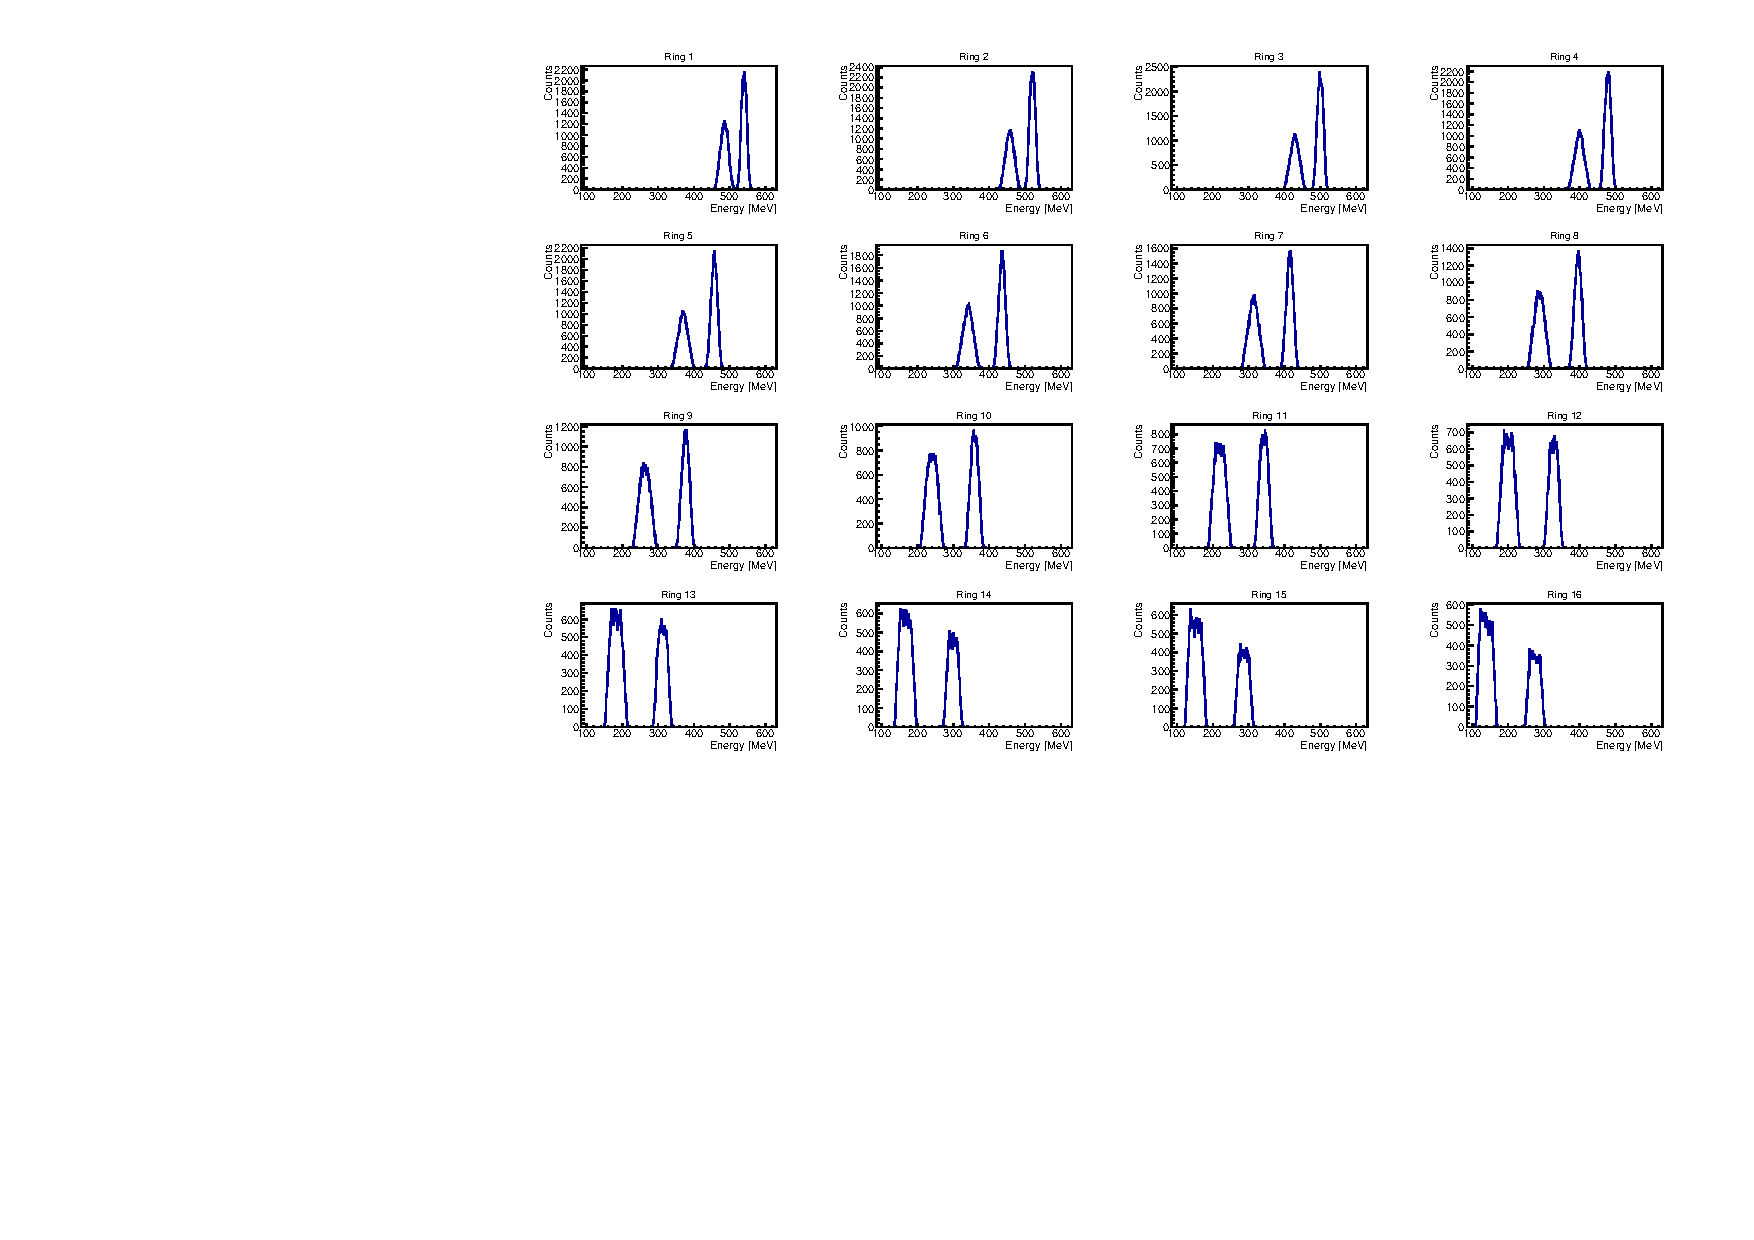
\includepdf[pages={-}, angle=270]{../Plots/simulation/cd_sim_all.pdf}

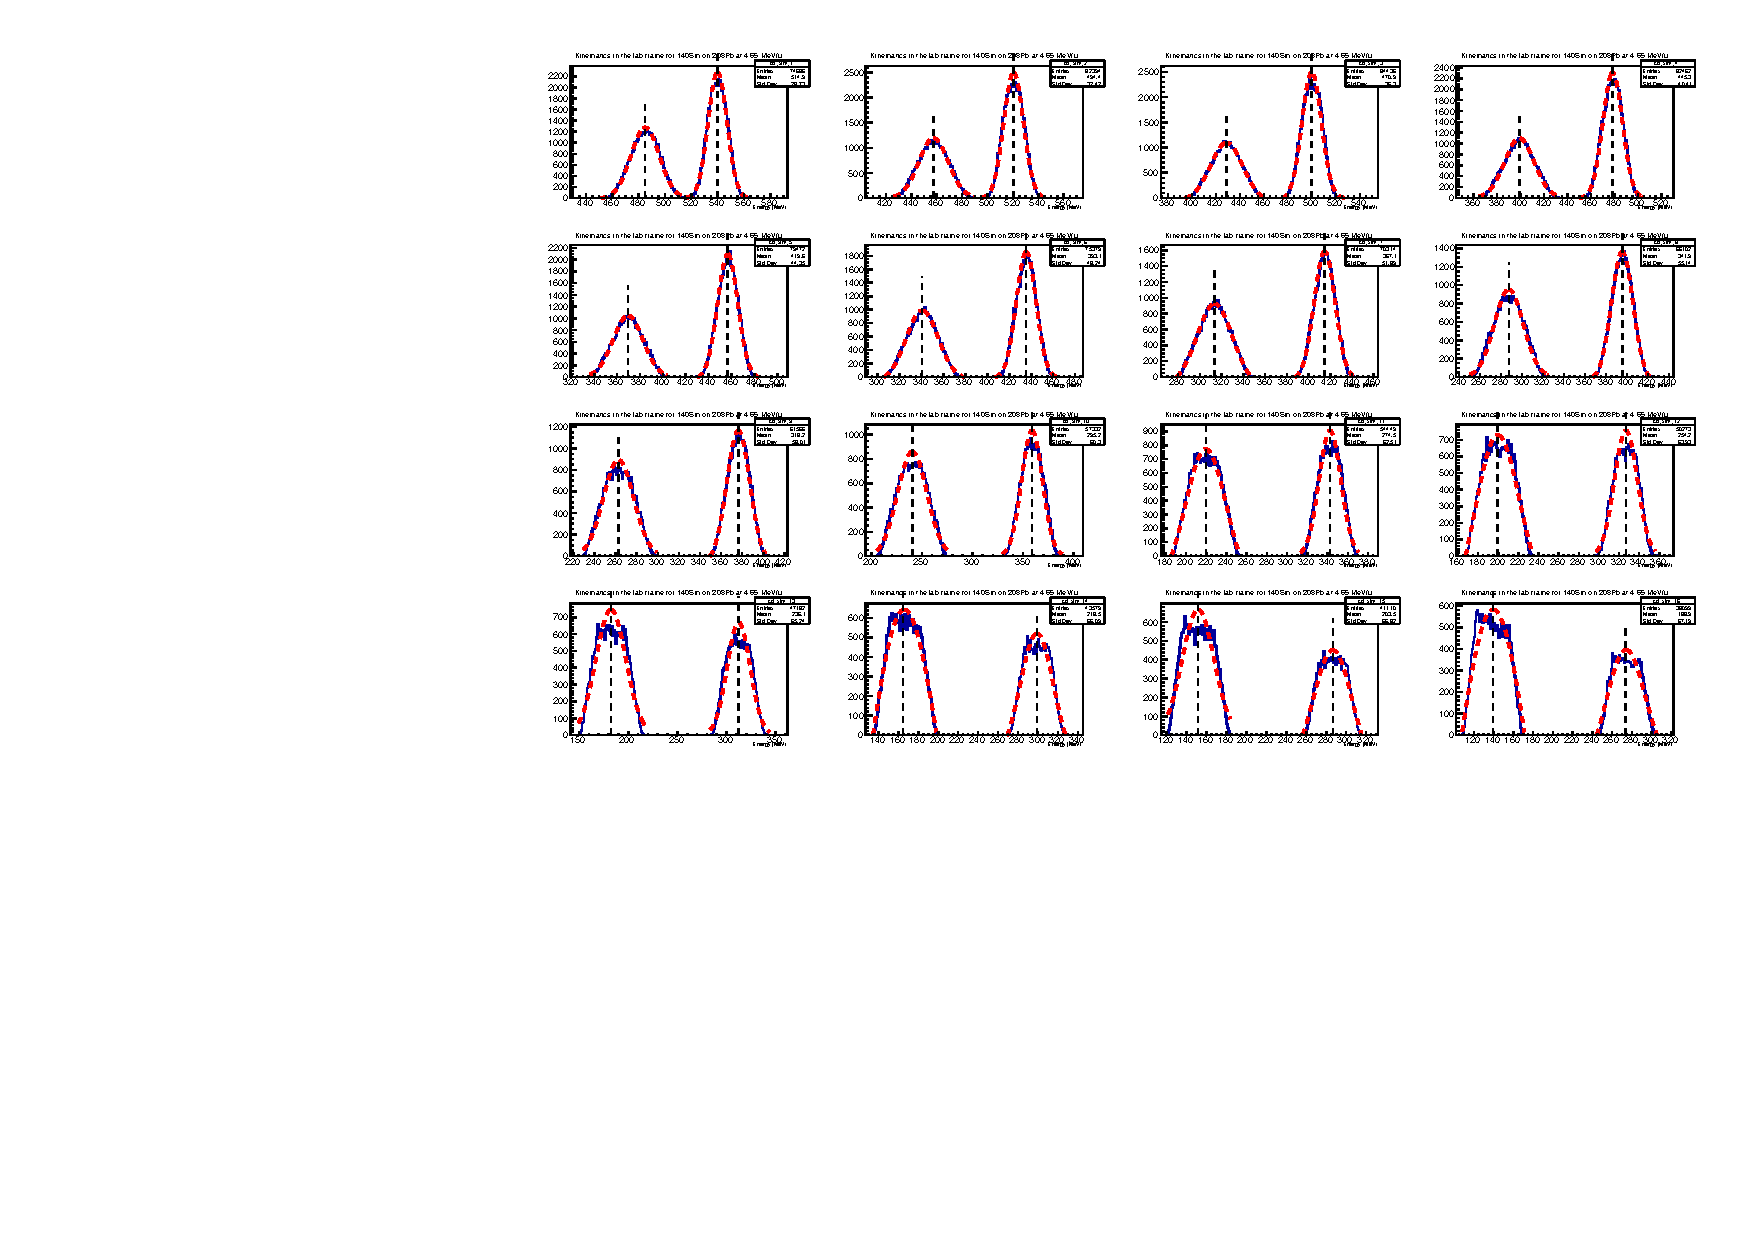
\includepdf[pages={-}, angle=270]{../Plots/fitting/Pb_Sm_sim.pdf}


\end{appendices}

% ----------------------------------------------------------------------------------------------------------------------% ----------------------------------------------------------------------------------------------------------------------

%\bibliographystyle{unsrtnat}
\bibliographystyle{mybibstyle} %my own bibstyle to set first names to one letter + unsrtnat

\bibliography{/Users/trondwj/GitHub/MasterThesis/Thesis/References/Mendeley.bib,/Users/trondwj/GitHub/MasterThesis/Thesis/References/web_references.bib}


\end{document}